%%%%%%%%%%%%%%%%%%%%%%%%%%%%%%%%%%%%%%%%%
% Masters/Doctoral Thesis 
% LaTeX Template
% Version 2.5 (27/8/17)
%
% This template was downloaded from:
% http://www.LaTeXTemplates.com
%
% Version 2.x major modifications by:
% Vel (vel@latextemplates.com)
%
% This template is based on a template by:
% Steve Gunn (http://users.ecs.soton.ac.uk/srg/softwaretools/document/templates/)
% Sunil Patel (http://www.sunilpatel.co.uk/thesis-template/)
%
% Template license:
% CC BY-NC-SA 3.0 (http://creativecommons.org/licenses/by-nc-sa/3.0/)
%
%%%%%%%%%%%%%%%%%%%%%%%%%%%%%%%%%%%%%%%%%

%----------------------------------------------------------------------------------------
%	PACKAGES AND OTHER DOCUMENT CONFIGURATIONS
%----------------------------------------------------------------------------------------

\documentclass[
11pt, % The default document font size, options: 10pt, 11pt, 12pt
%oneside, % Two side (alternating margins) for binding by default, uncomment to switch to one side
british, % ngerman for German
singlespacing, % Single line spacing, alternatives: onehalfspacing or doublespacing
%draft, % Uncomment to enable draft mode (no pictures, no links, overfull hboxes indicated)
%nolistspacing, % If the document is onehalfspacing or doublespacing, uncomment this to set spacing in lists to single
%liststotoc, % Uncomment to add the list of figures/tables/etc to the table of contents
	%toctotoc, % Uncomment to add the main table of contents to the table of contents
%parskip, % Uncomment to add space between paragraphs
%nohyperref, % Uncomment to not load the hyperref package
headsepline, % Uncomment to get a line under the header
%chapterinoneline, % Uncomment to place the chapter title next to the number on one line
%consistentlayout, % Uncomment to change the layout of the declaration, abstract and acknowledgements pages to match the default layout
]{MastersDoctoralThesis} % The class file specifying the document structure

\usepackage[utf8]{inputenc} % Required for inputting international characters
\usepackage[T1]{fontenc} % Output font encoding for international characters
\usepackage{abstract}
\usepackage{amsmath}
\usepackage{adjustbox}
\usepackage{mathpazo} % Use the Palatino font by default
\usepackage[backend=bibtex,natbib=true]{biblatex} % Use the bibtex backend with the authoryear citation style (which resembles APA)
\def\changemargin#1#2{\list{}{\rightmargin#2\leftmargin#1}\item[]}
\let\endchangemargin=\endlist 
\addbibresource{biblio.bib} % The filename of the bibliography
%\renewcommand\acknowledgementsname{Remerciements}
\usepackage[autostyle=true]{csquotes} % Required to generate language-dependent quotes in the bibliography
\newcommand{\mc}[2]{\multicolumn{#1}{|c|}{#2}}
\usepackage{longtable}
\usepackage{placeins}
\usepackage[bottom]{footmisc}
\interfootnotelinepenalty=10000
%\usepackage[para]{footmisc}
\usepackage{pdflscape} % or {lscape}
\setcounter{tocdepth}{2}
\usepackage{footnote}
\makesavenoteenv{tabular}
\let\Oldsection\section
\renewcommand{\section}{\FloatBarrier\Oldsection}

\let\Oldsubsection\subsection
\renewcommand{\subsection}{\FloatBarrier\Oldsubsection}

\let\Oldsubsubsection\subsubsection
\renewcommand{\subsubsection}{\FloatBarrier\Oldsubsubsection}
%\usepackage{blindtext}
%\usepackage{tabularx}
%\usepackage{gensymb}
%----------------------------------------------------------------------------------------
%	MARGIN SETTINGS
%----------------------------------------------------------------------------------------

\geometry{
	paper=a4paper, % Change to letterpaper for US letter
	inner=2.5cm, % Inner margin
	outer=3.8cm, % Outer margin
	bindingoffset=.5cm, % Binding offset
	top=1.5cm, % Top margin
	bottom=1.5cm, % Bottom margin
	%showframe, % Uncomment to show how the type block is set on the page
}


\begin{document}

\frontmatter % Use roman page numbering style (i, ii, iii, iv...) for the pre-content pages

\pagestyle{plain} % Default to the plain heading style until the thesis style is called for the body content

%----------------------------------------------------------------------------------------
%	TITLE PAGE
%----------------------------------------------------------------------------------------

\begin{titlepage}
\begin{center}

\begin{figure}[h]
\centering

\includegraphics[width=14cm]{Images/logos.jpg}
\end{figure}

\vspace*{.06\textheight}
{\scshape\LARGE {Université catholique de Louvain}\par}\vspace{1.5cm} % University name
%\textsc{\Large Doctoral Thesis}\\[0.5cm] % Thesis type

\HRule \\[0.4cm] % Horizontal line
\begin{changemargin}{-0.5cm}{-0.5cm} 
{\huge \bfseries {Study of the stress relieve heat-treatment of}\\
 \vspace{0.2cm}\hspace{0.2cm} \huge \bfseries {additively manufactured AlSi10Mg alloy:}}\vspace{0.3cm}

\LARGE{Influence on microstructure and mechanical properties}\par
\end{changemargin} 
\HRule \\[1.5cm] % Horizontal line
 \vspace{1cm}
\large \textit{Dissertation presented by}\\
\vspace{0.5cm}
\begin{minipage}[t]{0.35\textwidth}
\begin{flushleft} \large
David DISPAS
\end{flushleft}
\end{minipage}
\large \textit{and}
\begin{minipage}[t]{0.35\textwidth}
\begin{flushright} \large
Arthur BOUILLOT
\end{flushright}
\end{minipage}\\%[3cm]
 
\vspace{0.6cm}
\large \textit{for obtaining the Master’s degree in}\\[0.3cm] 
\vspace{0.20cm}
\begin{minipage}[t]{0.41\textwidth}
\begin{flushleft} \large
Mechanical Engineering
\end{flushleft}
\end{minipage}
\large \textit{and}
\begin{minipage}[t]{0.4\textwidth}
\begin{flushright} \large
Chemical and Materials \\
\centering \hspace{0.7cm} Engineering
\end{flushright}
\end{minipage}\\%[1cm]
\vspace{0.7cm}
\large \textit{at Ecole Polytechnique de Louvain (EPL)}\\[1.3cm]
\vfill
\large {\textit{Supervisor:} Aude SIMAR}
%\textit{in the}\\[0.4cm]
\vfill
%\groupname\\\deptname\\[2cm] % Research group name and department name
 \large {\textit{Readers:} Laurent DELANNAY, Anne MERTENS, Camille VAN DER REST}
%\vfill
\vfill
{\large Academic year 2017-2018}\\%[1cm] % Date
%\includegraphics{Logo} % University/department logo - uncomment to place it
 

\end{center}
\end{titlepage}

%---------------------------------------------------------------------
%%	QUOTATION PAGE
%%----------------------------------------------------------------------------------------

\vspace*{0.2\textheight}

\noindent\enquote{\itshape 'The gem cannot be polished without friction, nor man perfected without trials.'}\bigbreak

\hfill Confucius
%Parce que ça parle de polissage hihi

%----------------------------------------------------------------------------------------
%	ABSTRACT PAGE
%----------------------------------------------------------------------------------------

%\begin{abstract}
%%\addchaptertocentry{Résumé} % Add the abstract to the table of contents
%The Thesis Abstract is written here (and usually kept to just this page). The page is kept centered vertically so can expand into the blank space above the title too\ldots
%\end{abstract}

%----------------------------------------------------------------------------------------
%	ACKNOWLEDGEMENTS
%----------------------------------------------------------------------------------------

\chapter*{Acknowledgements}

%\addchaptertocentry{Remerciements} % Add the acknowledgements to the table of contents
...
%\end{acknowledgements}

%----------------------------------------------------------------------------------------
%	LIST OF CONTENTS/FIGURES/TABLES PAGES
%----------------------------------------------------------------------------------------

\tableofcontents % Prints the main table of contents

\listoffigures % Prints the list of figures

\listoftables % Prints the list of tables

%----------------------------------------------------------------------------------------
%	ABBREVIATIONS
%----------------------------------------------------------------------------------------

\begin{abbreviations}{ll} % Include a list of abbreviations (a table of two columns)
%
\textbf{AB}& \textbf{A}s-\textbf{B}uilt\\
\textbf{AM} & \textbf{A}dditive \textbf{M}anufacturing\\
\textbf{CAD} & \textbf{C}omputer \textbf{A}ided \textbf{D}esign\\
\textbf{CI} & \textbf{C}onfidence \textbf{I}nterval\\
\textbf{DMLS} & \textbf{D}irect \textbf{M}etal \textbf{L}aser \textbf{S}intering\\
\textbf{DMP} & \textbf{D}irect \textbf{M}etal \textbf{P}rinter\\
\textbf{HPDC} & \textbf{H}igh \textbf{P}ressure \textbf{D}ie \textbf{C}asting \\
\textbf{HW} & \textbf{H}ydrostatic \textbf{W}eigthing \\
\textbf{ICP} & \textbf{I}nductively \textbf{C}oupled \textbf{P}lasma\\
\textbf{RODIA} & \textbf{R}elative \textbf{O}ptical \textbf{D}ensity \textbf{I}mage \textbf{A}nalysis \\
\textbf{SD} & \textbf{S}tandard \textbf{D}eviation \\
\textbf{SEM} & \textbf{S}canning \textbf{E}lectron \textbf{M}icroscope\\
\textbf{SLM} & \textbf{S}elective \textbf{L}aser \textbf{M}elting\\

%\textbf{WSF} & \textbf{W}hat (it) \textbf{S}tands \textbf{F}or\\
%
\end{abbreviations}

%----------------------------------------------------------------------------------------
%	PHYSICAL CONSTANTS/OTHER DEFINITIONS
%----------------------------------------------------------------------------------------
%
%\begin{constants}{lr@{${}={}$}l} % The list of physical constants is a three column table
%
%% The \SI{}{} command is provided by the siunitx package, see its documentation for instructions on how to use it
%
%Speed of Light & $c_{0}$ & \SI{2.99792458e8}{\meter\per\second} (exact)\\
%%Constant Name & $Symbol$ & $Constant Value$ with units\\
%
%\end{constants}

%----------------------------------------------------------------------------------------
%	SYMBOLS
%----------------------------------------------------------------------------------------

\chapter*{Symbols}%{lll} % Include a list of Symbols (a three column table)
\begin{tabular}{lll}

\centering

$A_0$ & Initial minimal cross-sectional area & $[mm^2]$\\
$A_f$ & Minimal cross-sectional area after fracture & $[mm^2]$\\
$d_0$ & Initial minimal diameter & $[mm]$\\ 
$d_f$ & Minimal diameter after fracture& $[mm]$\\ 
$D_a$ & Average particle size & $[\mu m]$\\ 
$E$ & Young modulus & [$GPa$]\\
$E_d$ & Volumetric energy density & $[\frac{J}{mm^3}]$\\
$F$ & Force &$ [N] $\\
$h$ & Hatch space & $[\mu m]$\\
$H_v$ & Vickers hardness & $[HV]$\\
$\overline{H_v}$ & Average Vickers hardness & $[HV]$\\
$L$ & Extensometer gauge length & $[mm]$\\
$L_0$ & Initial extensometer gauge length &$[mm]$\\
$L_f$ & Final extensometer gauge length &$[mm]$\\
$P$ & Laser power & $[W]$ \\
$p_{O_2}$ & Oxygen pressure & $[mbar]$\\
$SD_{HV}$ & Vickers hardness measures standard deviation & [$H_v$]\\
$SD_{\rho_{rel}}$ & Relative density measures standard deviation & [$\%$]\\
$t$ & Layer thickness & $[\mu m]$\\
$v_s$ & Scanning speed & $[\frac{mm}{s}]$ \\
$W_a$ & Specimen dry weight& $ [g]$ \\
$W_w$ & Specimen underwater weight & $[g]$\\
\addlinespace
\addlinespace
$\epsilon_{eng}$ & Engineering strain & [\%]\\
$\epsilon_{f,eng}$ & Engineering strain at fracture & [\%]\\
$\epsilon_{f,true}$ & True strain at fracture & [\%]\\
$\phi_{99\%}$ & Laser spot size at the 99\% contour & $[\mu m]$\\
$\lambda$ & Laser wavelength & $[nm]$\\
$\rho_{a}$ & Apparent density & $[\frac{g}{cm^3}$] \\
$\rho_{a,rel}$ & Apparent relative density & $[\%]$ \\
$\rho_{b,rel}$ & Theoretical bulk density & $\frac{g}{cm^3}$\\ 
$\rho_{w}$ & Water density & $[\frac{g}{cm^3}$]\\
$\rho_{rel}$ & Relative density & $[\%]$ \\
$\overline{\rho_{rel}}$ & Average relative density & $[\%]$ \\
$\sigma_{eng}$ & Engineering stress & $[MPa]$\\
$\sigma_u$ & Ultimate tensile strength & $[MPa]$\\
$\sigma_y$ & Yield strength & $[MPa]$\\

%\addlinespace % Gap to separate the Roman symbols from the Greek

%$\omega$ & angular frequency & \si{\radian} \\
\end{tabular}
%\end{symbols}

%----------------------------------------------------------------------------------------
%	DEDICATION
%----------------------------------------------------------------------------------------

\dedicatory{Nous dédions ce travail à nos familles et amis} 

%----------------------------------------------------------------------------------------
%	THESIS CONTENT - CHAPTERS
%----------------------------------------------------------------------------------------

\mainmatter % Begin numeric (1,2,3...) page numbering

\pagestyle{thesis} % Return the page headers back to the "thesis" style

% Include the chapters of the thesis as separate files from the Chapters folder
% Uncomment the lines as you write the chapters

\chapter{Introduction}
\label{Chap1}

This is, with the concluding chapter, a significant portion of memory. This should
especially present the context and objectives of the work. Generally, the memory structure (content
of chapters) is briefly exposed

\chapter{State of the art}
\label{Chap2}
\section{Selective laser melting technology}
Selective laser melting (SLM) - also referred to as direct metal laser sintering (DMLS) - is an additive manufacturing  (AM) technique making use of a high power-density laser that locally melts powder materials.%Layers are progressively piled up, in order to create a 3D part. 
 When a layer of powder has been melted, a new layer is spread on top of the previous one, and is in turn melted, in order to progressively build a 3D object. The technique is illustrated on figure \ref{fig:SLM} \parencite{LEITZ2017331}. The materials used include mostly metals but also ceramics and composites. Parts to build must first be drawn in a computer-aided design (CAD) software and broken down in 2D slices, each one corresponding to a powder layer. During the process, the oxygen pressure $p_{O_2}$ must be kept low to prevent the oxidation of the metal. A shielding gas - such as argon - is thus used to fill the build chamber at all time, while $p_{O2}$ is monitored.   \\

\begin{figure}[ht]
\centering
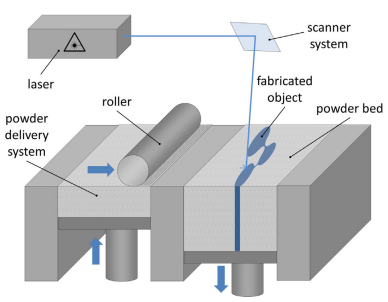
\includegraphics[scale=0.7]{Images/SLM}
\decoRule
\caption[Selective laser melting technology principle]{Selective laser melting technology principle (from Leitz et al., 2017 \parencite{LEITZ2017331}).}
\label{fig:SLM}
\end{figure}

SLM is still a young technology. Its popularity only increased significantly over the last decade, as depicted by figure \ref{fig:Evol}. Works concerning AlSi10Mg began to emerge noticeably in 2014. The technique usage spread rapidly in many sectors: biomedical, heat exchangers, aerospace and automotive - to name just a few \parencite{Yap}. This is due to the numerous appeals of SLM compared to the other technologies, including:\\

\begin{itemize}
\item Geometrical flexibility: parts can be designed with thin walls or even with hidden cavities and/or channels. This offers promising prospects regarding light-weight potentials for parts solicited mechanically \parencite{Lippert};
\item Increased reliability of the parts \parencite{Haase};
\item Reduced equipment costs \parencite{Hoeges};
\item Better operational efficiency: the fabrication is quick and easy which reduces time-to-market as well as assembly times and capital tied up in stocks \parencite{Hoeges};
\item Individual production facilitation \parencite{Haase};
\item Reduced material waste and better energy usage: the process is  environmentally friendly as a whole \parencite{Haase}.
\end{itemize}

\begin{figure}[ht]
\centering
\noindent\makebox[\textwidth]{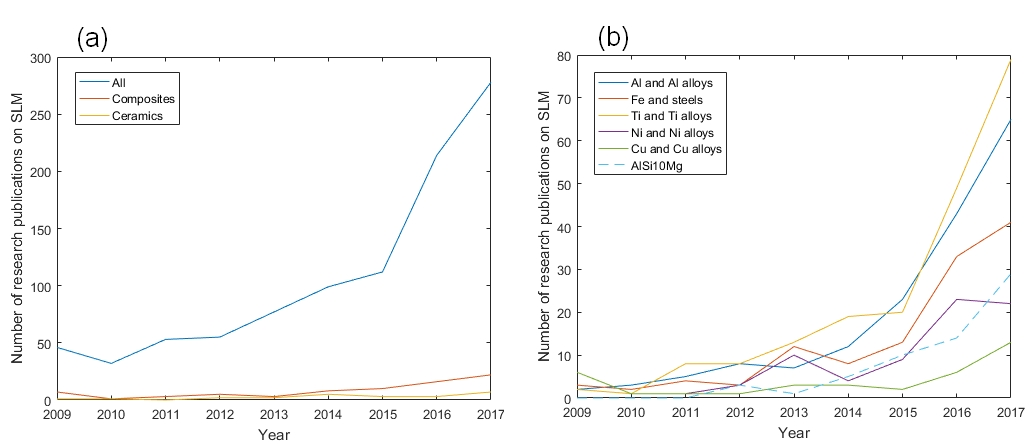
\includegraphics[scale=0.55]{Images/Evol}}
\decoRule

\caption[(a)Research publications on SLM of ceramics, composites and all materials types combined. (b)Research publications on SLM of different metallic materials]{(a)Research publications on SLM of ceramics, composites and all materials types combined. (b)Research publications on SLM of different metallic materials. Data are derived from the research publications on SLM, LaserCusing and DMLS existing on ScienceDirect website.}
\label{fig:Evol}
\end{figure}

The properties of parts produced through SLM stem from the coupled effects of a great deal of parameters (see figure \ref{fig:param} ) \parencite{Aboulkair140820}.  %Les caractérisitiques des pièces produites grâce à la fusion laser sélective (SLM) sont le fruit de l'action simultanée et couplée d'un grand nombres de paramètres (see figure \ref{fig:param} ) \parencite{Aboulkair140820}.
Results are very sensitive to their variations. The process parameters must thus be monitored thoroughly. This complicates the search for their optimisation, still not fully resolved for aluminium alloys.\\%.Les résultats sont très sensibles à leurs variations et il est donc nécessaire de les contrôler méticuleusement. Pour ces raisons, il n'est pas simple d'étudier leurs impacts.\\
\begin{figure}[ht]
\centering
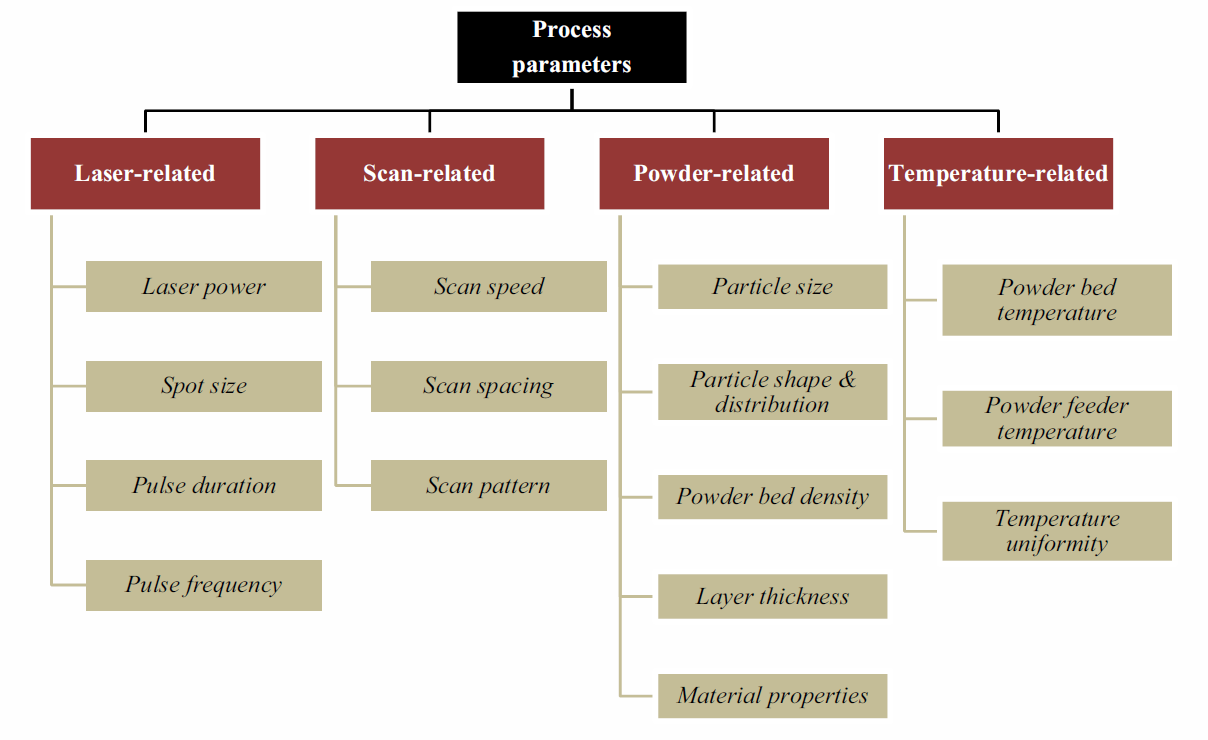
\includegraphics[scale=0.37]{Images/Param}
\decoRule

\caption[Parameters involved in SLM]{Parameters involved in SLM (from Aboulkhair et al., 2014 \parencite{Aboulkair140820}).}
\label{fig:param}
\end{figure}

In recent years, works aiming at facing this challenge multiplied. The minimisation of the porosity is at the center of attention. It is indeed closely related to the quality of the mechanical properties. As porosity contributes to lowering the load-bearing surface, it reduces the apparent material strength. It was also observed to have a critical influence on the fatigue life of the produced parts. Their lifetime is especially diminished if the values of pores amount and size go beyond a certain threshold \parencite{Brandl121509}. Studies investigating the effects of various parameters on the AlSi10Mg fabrication through SLM abound in the literature.\\

\section{AlSi10Mg alloy}
\textcolor{red}{Parler de l'AlSi10Mg; quel est l'interet de travailler avec? Difficultés? (reflectivité etc).. Qu'est ce qui existe en coulé, forgé etc}\\
\textcolor{red}{Microstructure homogène, diagramme de phase}\\

\textcolor{gray}{Kempen dans "PROCESS OPTIMIZATION AND MICROSTRUCTURAL ANALYSIS FOR SELECTIVE LASER
MELTING OF AlSi10Mg ":}

\textcolor{gray}{AlSi10Mg is a typical casting alloy which is, due to its high strength/density ratio and thermal
properties, highly demanded in aerospace and automotive industries [1]. The alloy combination of aluminium,
silicon and magnesium results in a significant increase in strength and hardness which might even reach 300
MPa and 100 HBS, respectively, by applying a proper heat treatment [2]}

\textcolor{gray}{Aluminium as a lightweight material is very attractive for the production of parts that require good
mechanical properties in combination with a low weight. The main focus lies on Al-Si alloys, since they are
casting alloys that are also suitable for welding. AlSi10Mg, which can be hardened by applying a specific heat
treatment, is relatively easy to process by laser applications due to the small difference between liquidus and
solidus temperature compared to high strength aluminium-alloys [2]. The AlSi10Mg alloy is frequently used in
aerospace, automotive, chemical and food industry. Its composition according to ISO 3522 can be found in
Table 1 [4]. Alloying the magnesium to the Al-Si alloy enables precipitation of Mg2Si which will strengthen the
matrix without compromising the other mechanical properties to a significant extent.}
\section{Fabrication process parameters}
\label{pp}
Let us now investigate the influence of the parameters on the properties of AlSi10Mg parts manufactured with SLM. The analysis of the paired impacts of the laser power P and scan speed $v_s$ provides a first insight. As depicted by figures \ref{fig:Pvs} and \ref{fig:Pvs2}, low P and high $v_s$ lead to an insufficient energy input to melt the powder and re-melt the substrate, which causes the formation of droplets \parencite{Kempen110817} . The opposite leads to good penetration but also to distortions and irregularities.   A trend to use both high P and $v_s$ rose in accordance with these findings. Doing so has the advantage to increase productivity. However, it also has multiple downsides including a decrease of the surface quality due to balling, excessive spatter, and an augmented gas induced porosity \parencite{Mertens170406}. Therefore, a trade-off must be found. \\

A popular approach is to regroup multiple operating parameters into one, the volumetric energy density $E_d$. It is estimated through the following formula: 
$$E_d=\frac{P}{v_s h t} $$
where t is the layer thickness and h is the hatch space. As a rule of thumb, $E_d$ should be chosen in the range between 60 and 75 [$\frac{J}{mm^3}$] \parencite{Read150417}. However, the criterion is insufficient and others phenomena, such as melt pools overlapping, should be considered \parencite{Tang170309}. Very few studies were carried out to optimize h and t independently. Their values lie generally in the intervals [50 ; 200] [$\mu m$] and [20 ; 60] [$\mu m$], respectively \parencite{aboulkhair2016,Brandl121509,Kempen110817,Mertens170406}. It was observed that for t = 30 [$\mu m$], an optimal set of parameters values in terms of density is P = 200 [W], $v_s=1400 [\frac{mm}{s}]$ and h = 105 [$\mu m$] \parencite{Kempen110817}. The apparent relative density $\rho_{a,rel}$ was then above 99.5 [\%], considering the theoretical bulk density $\rho_b$ to be equal to 2.68 [$\frac{g}{mm^3}$].\\

\begin{figure}[ht]
\centering
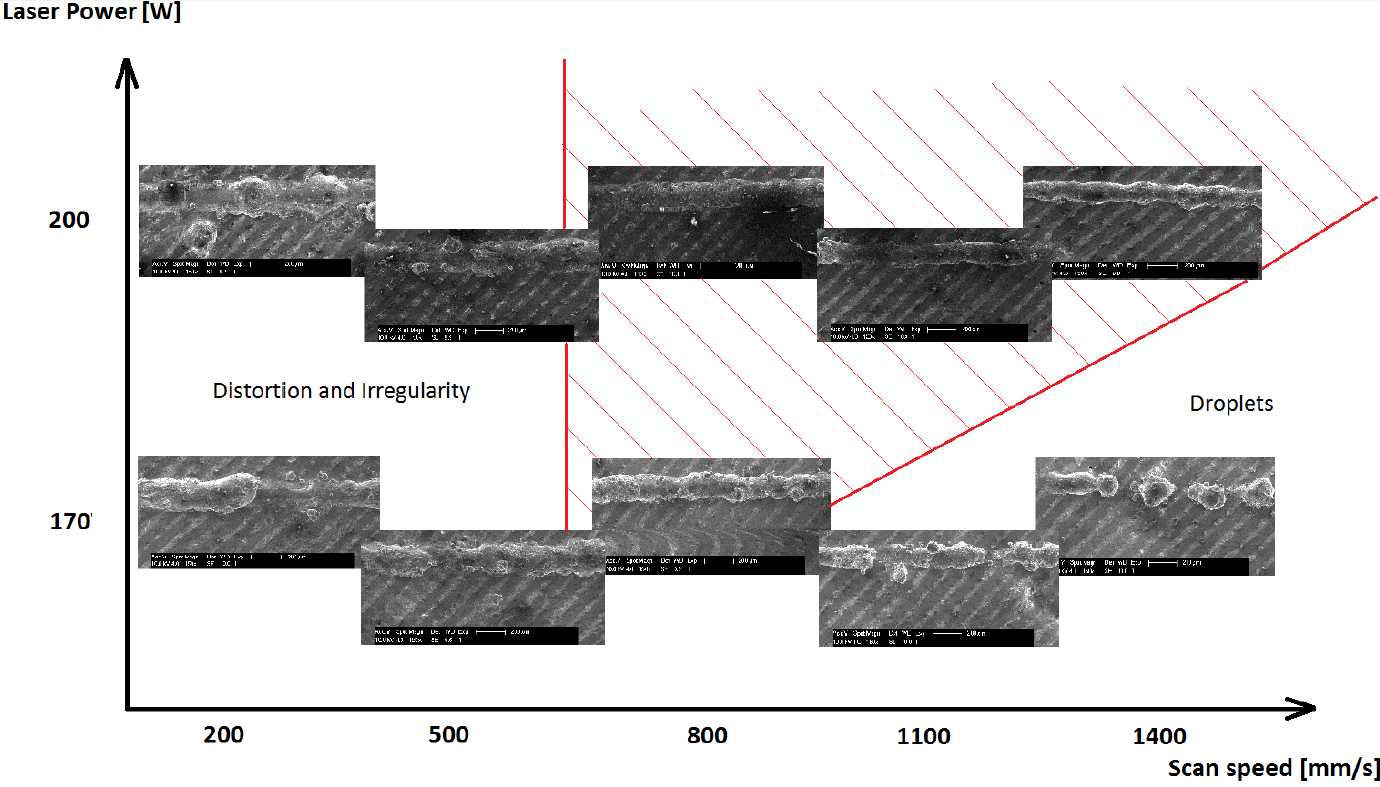
\includegraphics[scale=0.34]{Images/Pvs}
\decoRule
\caption[Process window for SLM of AlSi10Mg, based on the top view of single track scans]{Process window for SLM of AlSi10Mg, based on the top view of single track scans (from Kempen et al., 2011 \parencite{Kempen110817}).}
\label{fig:Pvs}
\end{figure}

\begin{figure}[ht]
\centering
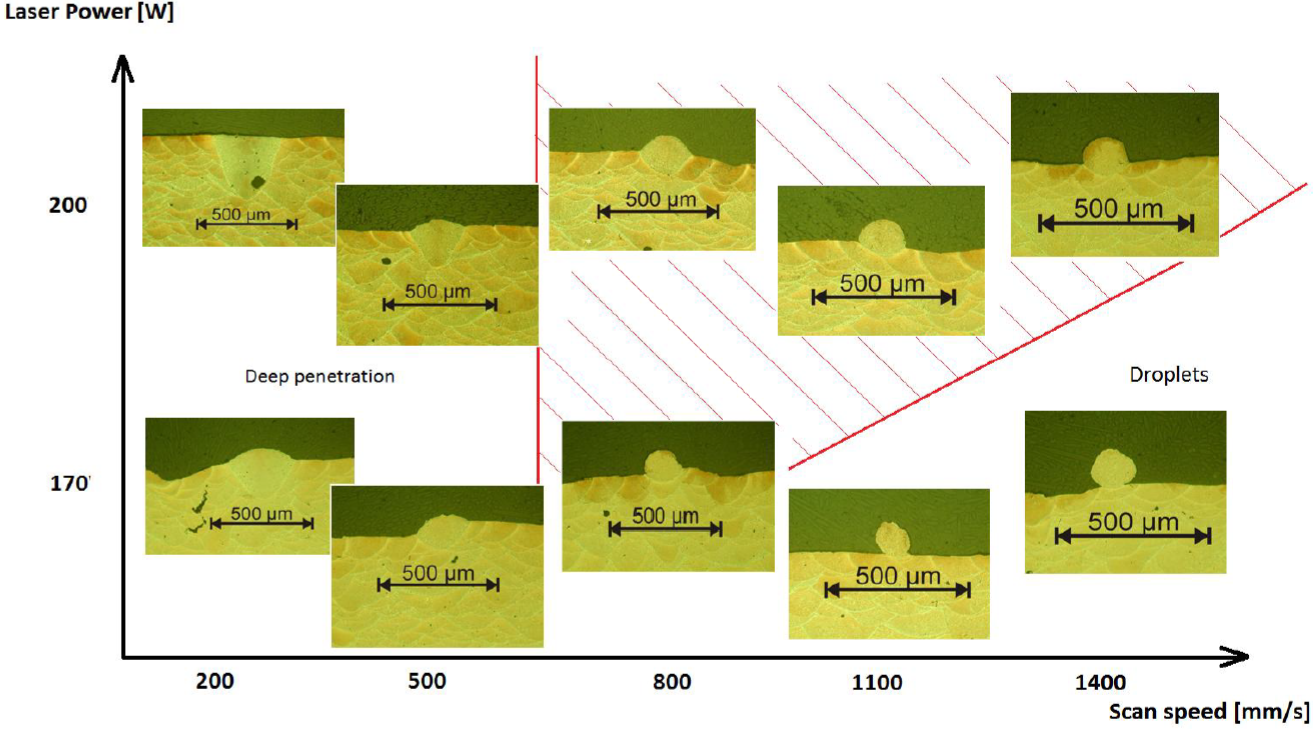
\includegraphics[scale=0.34]{Images/Pvs2}
\decoRule
\caption[Process window for SLM of AlSi10Mg, based on the front view of single track scans]{Process window for SLM of AlSi10Mg, based on the front view of single track scans (from Kempen et al., 2011 \parencite{Kempen110817}).}
\label{fig:Pvs2}
\end{figure}

The other process parameters will be covered for the sake of completeness. Let us first look into the particle-related parameters. The particle size $D_a$ of the powder should be as small as possible to ensure a good flowability and allow for thin layers \parencite{Kempen110817}. Typical values for mean particle size stretch from 15 to 50 [$\mu m$] but are more often at around 30 [$\mu m$] \parencite{Brandl121509,Kempen110817,MOWER2016198,UZAN2017229}. The size distribution is more delicate to outline. On one hand, wider distributions often generate better bed density, parts with higher density and better surface finish. On the other hand, narrower ones usually provide better flowability and parts with better strength and hardness \parencite{Liu1101}. In most cases, a middle ground between the two should be sought. In SLM applications, powder is often successively recycled multiple times. This leads to their progressive contamination with moisture, which causes an increase of hydrogen porosity in the produced parts \parencite{Weingarten151102}. The problem can be overcome by drying the powder or using fresh one. Unfortunately - in the case of aluminium alloys - no findings were made regarding the prediction of a threshold at which one should take action \parencite{aboulkhair2017}.    \\

The choice of scan pattern has great importance. There exist a few different strategies. The common ones use unidirectional, bidirectional or islands patterns (see figure \ref{fig:Strat}). The scan direction(s) should always be rotated between successive layers to favorise isotropy, especially in the unidirectional case since it causes height variations along a layer \parencite{aboulkhair2016}. The islands pattern is based on a decomposition in small domains with short scanning tracks. Two usual strategies can be distinguished among this group: the chessboard and the hexagonal one. A study proved the superiority of an island pattern over a bidirectional one in terms of both ultimate tensile stress $\sigma_u$ and strain at fracture $\epsilon_f$ for a 316L stainless steel-Inconel 718 material \parencite{Zhou15}. It was also shown that it was possible to fabricate pure titanium samples without cracks using an island pattern, and not with a bidirectional one \parencite{Li17}. This is seemingly due to the greater accumulation of internal stresses and to the weaker interlayer bounding in the second case. \\

\begin{figure}[ht]
\centering
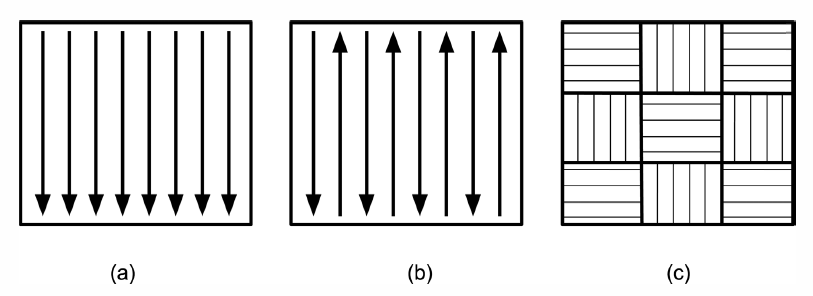
\includegraphics[scale=0.6]{Images/Strat}
\decoRule
\caption[Schematic representation of scanning strategies commonly used in LSM (a) unidirectional long scan track; (b) bi-directional long scan track, and (c) islands]{Schematic representation of scanning strategies commonly used in LSM (a) unidirectional long scan track; (b) bi-directional long scan track, and (c) islands (from Mertens et al., 2017 \parencite{Mertens170406}).}
\label{fig:Strat}
\end{figure}

Furthermore, dual scanning strategies were proven to be effective. For example, a pre-scan with low $E_d$ can flatten the powder bed before it is consolidated, which leads to a reduction of porosity \parencite{Mertens170406}. It was also shown that scanning the contour of the part being built at lower $E_d$ can better the surface roughness for AlSi12Mg \parencite{PRASHANTH170205}. One should note too that the final properties of the fabricated part can strongly depend on the building direction (see figure \ref{fig:Build}) \parencite{DELROISSE201732}. Further properties comparison is provided in section \ref{MMABMP}.\\

\begin{figure}[ht]
\centering
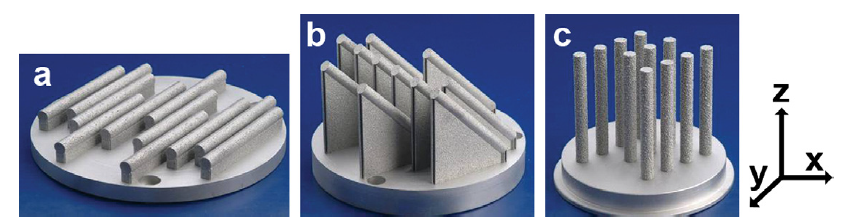
\includegraphics[scale=0.58]{Images/Build}
\decoRule
\caption[Samples (static tensile) built in different directions: (a) $0^\circ$, (b) $45^\circ$, and (c) $90^\circ$]{Samples (static tensile) built in different directions: (a) $0^\circ$, (b) $45^\circ$, and (c) $90^\circ$ (from Brandl et al., 2012  \parencite{Brandl121509}).}
\label{fig:Build}
\end{figure}


Other laser-related parameters - the spot size and the pulse properties - can also influence the process. Only the laser spot size at the 99\% contour $\phi_{99\%}$ is frequently cited in literature. Its value lies between 20 and 200 [$\mu m$] \parencite{Brandl121509,Kempen110817,MOWER2016198}. At this moment, no optimisation study was carried out about this variable. One should expect the optimal value for P, $v_s$, t, and h to depend on the spot size as it has a direct incidence on $E_d$. \\

Finally, the temperature of the powder bed and feeder affect the final properties of the fabricated parts as well. In particular, it was observed that pre-heating the powder at $300^\circ$ C mitigates the differences of fatigue resistance between tensile specimens built in different directions: it is possible that the operation induces a slower cooling rate which helps reducing the distortions and internal stresses \parencite{Brandl121509}.\\

Once the porosity problem is sorted out, other matters can be addressed such as productivity and surface roughness. The latter is problematic as the surface finish obtained with SLM is typically of such poor quality that all cracks initiate near the surface for a sample with relative density $\rho_{rel}>99\%$ \parencite{Brandl121509}. As said before, it is possible to reduce the surface roughness by mean of a dual scan strategy. However, the only options to obtain significantly better surface finish is currently to machine or polish the fabricated parts. This is one of the main weak points of SLM.\\ %Durant les dernières années, les travaux visant à optimiser les conditions de fabrication se sont multipliés. La minimisation de la porosité est au centre de l'attention: elle est en effet liée à la qualité des propriétés mécaniques. De plus au delà d'un seuil, des risques de rupture prématurée peuvent apparaitre (source). (Initiation de sites de propag ... ) On s'intéresse ensuite à optimiser d'autres caractéristiques du matériau et à la productivité de la technique.


\section{As-built mechanical properties}
\label{MMABMP}
In a work of Kempen et al., it was concluded that as-built (AB) additively manufactured AlSi10Mg samples can have mechanical properties (Vickers hardness \textit{HV}, ultimate tensile stress $\sigma_u$ , fracture strain $\epsilon_f$ and impact energy) better or at least comparable to the conventionally casted and high pressure die casted (HPDC) alloy \parencite{KEMPEN2012439}. The tensile specimens built in an horizontal direction (XY) had slightly different characteristics than those built in the vertical direction (Z). The results obtained in the mentioned work are gathered in table \ref{tab:Kemp1}, along with other results and common cast AlSi10Mg properties. The mechanical properties all lie in wide ranges. This illustrates the importance of mastering the process parameters. The best tensile properties measurements found on the web - both in terms of $\sigma_u$ and $\epsilon_f$ - were obtained by \textit{EOS} with $\rho_{rel} \simeq 99.85$  ($\rho_b$ considered to be equal to 2.67 [$\frac{g}{cm^3}$]) \parencite{EOS}. Unfortunately, the manufacturing condtions were omitted in sources \parencite{EOS} and \parencite{KEMPEN2012439}.

 \begin{center}
\begin{table}[ht]
\noindent\makebox[\textwidth]{\begin{tabular}{|c|c|c|c|c|c|}
    \hline
    Process & E [GPa] &$\sigma_y [MPa]$ &$\sigma_u$[MPa]&$\epsilon_f$[\%]&HV [HV] \\
\hline
\hline   
    SLM - XY direction \parencite{KEMPEN2012439}& $68 \pm 3$& - &$391 \pm 6$&$5.55\pm 0.4$&127	\\
    SLM - Z direction \parencite{KEMPEN2012439}& &- &$396 \pm 8$ & $3.47\pm 0.6$&	\\
    SLM  \parencite{ABOULKHAIR2016139}& $77 \pm 5$ & $268 \pm 2$  &$333 \pm 15$ & $1.4 \pm 0.3$ & $125 \pm 1$\\
    SLM - XY direction \parencite{MOWER2016198} & 65.5 & 227 &358&3.9 & - \\
    SLM - Z direction \parencite{MOWER2016198} & 75.4 & 172 & 289 & 2.6 & - \\
    SLM - XY direction \parencite{EOS} & $75 \pm 10$ &$270 \pm 10$ &$460 \pm 20$ &$9 \pm 2$ & $ 119 \pm 5$  \\
    SLM - Z direction \parencite{EOS} & $70 \pm 10$ &$240 \pm 20$ & $460 \pm 20$   &$6 \pm 2 $ &  \\
    \hline
    Conventional cast and aged \parencite{KEMPEN2012439}& 71 &- &300-317&2.5-3.5&86\\
    As built HPDC \parencite{KEMPEN2012439}& &- &300-350&3-5&95-105\\
    T6 treated HPDC \parencite{KEMPEN2012439}& &- &330-365&&130-133\\
    \hline

\end{tabular}}

\caption[Mechanical properties of SLM built parts and cast + aged parts in literature]{Mechanical properties of SLM built parts and cast + aged parts in literature}
\label{tab:Kemp1}
\end{table}
 \end{center}
 
Furthermore, Wang et al. observed that preheating the manufacturing plate can have great impact on the mechanical properties \parencite{Wang2018}. This is due to the differences in thermal gradients between the substrate and the built samples, which induces residual stresses. Results obtained for a chessboard pattern are shown in table \ref{tab:Wang}. Residual stresses are discussed further in section \ref{EARSSP}.

 \begin{center}
\begin{table}[ht]
\noindent\makebox[\textwidth]{\begin{tabular}{|c|c|c|c|c|}
    \hline
    Plate temperature & $\sigma_u$ [MPa] & $\epsilon_f [\%]$ & HV [HV] & $\rho_{rel} [\%]$ \\
\hline
\hline   
    80$^\circ C$ &385 $\pm 6$ & $3 \pm 1.5$ & 176 $\pm 6$& 98.69 $\pm 0.19$	\\
    120$^\circ C$ &381.3 $\pm 3.3$ & $2.83 \pm 0.33$ & 257 $\pm 9$& 97.39 $\pm 0.38$	\\
    160$^\circ C$ &363.7 $\pm 11.3$ & $5.33 \pm 0.67$ & 233 $\pm 4$& 97.01	\\
    \hline

\end{tabular}}
\caption[Mechanical properties for different plate pre heating temperatures (from Wang et al., 2018) \parencite{Wang2018}.]{Mechanical properties for different plate pre heating temperatures (from Wang et al., 2018) \parencite{Wang2018}.}
\label{tab:Wang}
\end{table}
 \end{center}

SLM AlSi10Mg is sometimes compared to wrought Al6061. It is also an aluminium-based alloy containing magnesium and silicon as major alloying elements. Its properties (after T6 treatment) are similar to its counterpart's as it is shown in table \ref{tab:6061}. It could thus be considered as an alternative for given applicationd. Fatigue properties of SLM AlSi10Mg where observed to be substantially poorer to the other material's: its lifetime was approximately one order of magnitude less for any applied stress amplitude (see figure \ref{Fat}) \parencite{MOWER2016198}. It was proven that the defects control the fatigue life. The defects giving rise to failure often locate near the surfaces of the samples. Polishing can thus better their fatigue strength but not systematically. \\

 \begin{center}
\begin{table}[ht]
\centering
\begin{tabular}{|c|c|c|c|c|}
    \hline
    E [GPa] &$\sigma_y [MPa]$ &$\sigma_u$[MPa]&$\epsilon_f$[\%]&HV [HV] \\
\hline
\hline   
    68.9 &276  & 310 &12 &107	\\
    \hline

\end{tabular}
\caption[Mechanical properties of T6 treated Al6061 alloy]{Mechanical properties of T6 treated Al6061 alloy (from Aerospace Specification Metals Inc., 2000 \parencite{6061}) }
\label{tab:6061}
\end{table}
 \end{center}
 
\begin{figure}[ht]
\centering
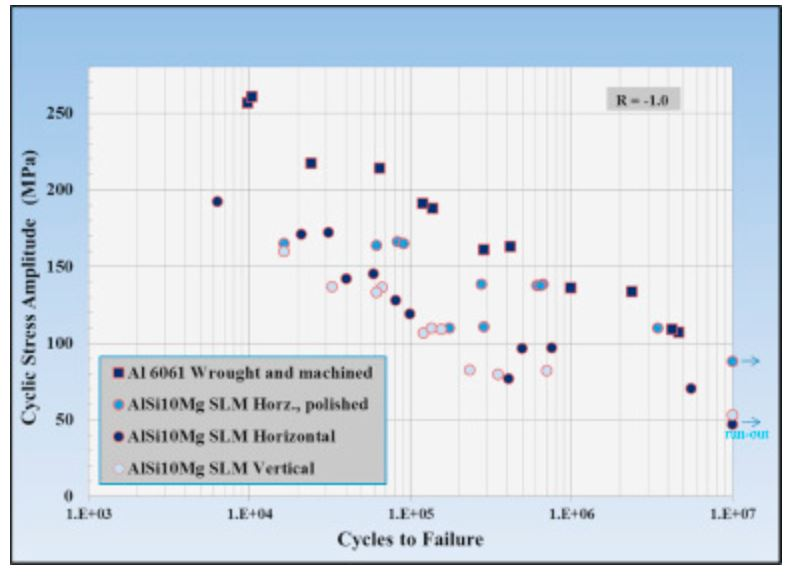
\includegraphics[scale=1]{Images/Fat}
\decoRule
\caption[Measured room-temperature stress-life (S–N) of SLM AlSi10Mg, compared to that of conventional Al 6061. Bending fatigue (rotating beam) at a frequency of 25 Hz. ]{Measured room-temperature stress-life (S–N) of SLM AlSi10Mg, compared to that of conventional Al 6061. Bending fatigue (rotating beam) at a frequency of 25 Hz. (from Todd Mower and Michael Long, 2016 \parencite{MOWER2016198}) .}
\label{Fat}
\end{figure} 
 
% \begin{center}
%\begin{table}[ht]
%\noindent\makebox[\textwidth]{\begin{tabular}{|c|c|}
%    \hline
%    Process & Impact energy [J] \\
%\hline
%\hline   
%    SLM - XY direction & $3.94 \pm 0.5$	\\
%    SLM - Z direction & $3.69 \pm 0.48	$\\
%    \hline
%    Conventional cast & 2.5-3.0\\
%    \hline
%
%\end{tabular}}
%\caption[Results of Charpy impact testing]{Results of Charpy impact testing (from Kempen et al., 2012)}
%\label{tab:Kemp2}
%\end{table}
% \end{center}

\section{Residual stresses in SLM parts}
\label{EARSSP}
\textcolor{red}{Introduire les contraintes internes: pourquoi il y en a? Sont-elles quantifiées dans la littérature? Traction/Comp ? Haut/bas? Techniques de caractérisation? Influence sur les précisions géométriques, sur les propriétés méca (statique \& fatigue)? Comment les éviter en cours de process ou supprimer après? =Intro pour section suivante.}\\

After most manufacturing processes, the fabricated piece can present residual stresses, both in compression and tension. While they are sometimes sought in some specific applications, they are more often an unwanted consequence of the process. Indeed, uncontrolled internal stresses can deteriorate dramatically the fatigue behaviour of the piece, cause unacceptable deformation, as well as premature failure, by facilitating the initiation of crack growth \cite{Vrancken2016}.\\

Many phenomena can be the cause of residual stresses, but it always go through inhomogeneous plastic strains. Several forming processes, such as cold rolling, can induce them, by applying a non-uniform load. On a more microscopic scale, different reactions to stress between distinct phases or crystal orientations are also able to create those inhomogeneities.\\

In the case of SLM parts, internal stresses are mostly due to the intense thermal gradients appearing during the scan. After the laser passage, the melt pool cools down, and begins to solidify. This solidification brings with it a thermal shrinkage of the molten track, which put it under tensile condition. The continuous shrinking along the scan track concentrates those tension stresses horizontally, in the direction of the scan vectors. Fabrication of successive layers on top, with their own tensile stresses, gradually relaxes the buried layers, to the point that they begin to undergo compressive stresses below a certain depth.Vertical tensile stresses on the side surfaces, induced by those horizontal stresses at each layer, remain however after the complete fabrication. An example of the stress distribution in a 2D section of a piece after manufacturing is available in Fig. \ref{fig:rs_section}. According to the supplier \cite{Inconel}, Inconel718 has a yield strength of approximatively 1 GPa. Although residual stresses do not seem to reach it, their value is definitively high enough to completely modify the mechanical behaviour of the piece. In the case of a tensile test, for example, the zone near the surface would enter plasticity way before applying a stress equal to the yield strength. \\

\begin{figure}[ht]
	\centering
	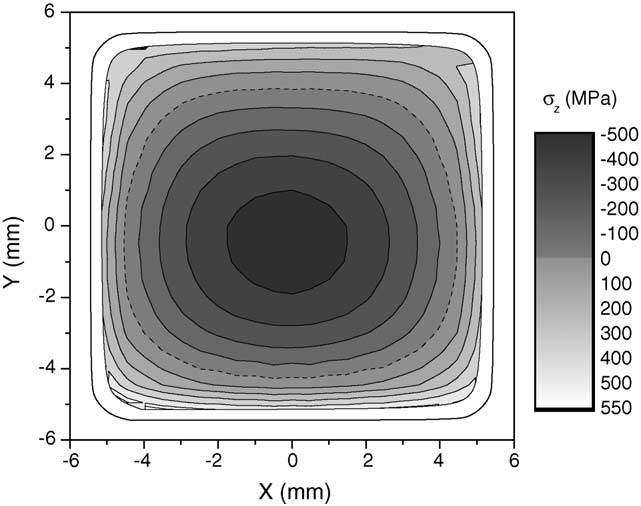
\includegraphics[scale=0.50]{Images/rs_section}
	\decoRule
	\caption[2D plot of vertical internal stresses measured by the contour method at mid-height, in a vertically-built parallelipiped Inconel718 sample. Vertical stresses are null along the dashed line.]{2D plot of vertical internal stresses measured by the contour method at mid-height, in a vertically-built parallelepiped Inconel718 sample. Vertical stresses are null along the dashed line (from Vrancken, 2016 \parencite{Vrancken2016}).}
	\label{fig:rs_section}
\end{figure}

As shown in Fig. \ref{fig:rs_section}, residual stresses can be measured by the so-called "contour method", which is only one of the many available techniques. They are usually categorised by their destructiveness on the tested part, and their depth of measurement in a reference material, steel. A sample of these techniques is presented in Fig. \ref{fig:rs_measure}. The most important non-destructive methods rely on diffraction, which use the lattice deformations at the atomic scale as indicators of the stress the material undergoes. Usual sources of radiation to diffract are X-rays, electrons and neutrons.\\

\begin{figure}[ht]
	\centering
	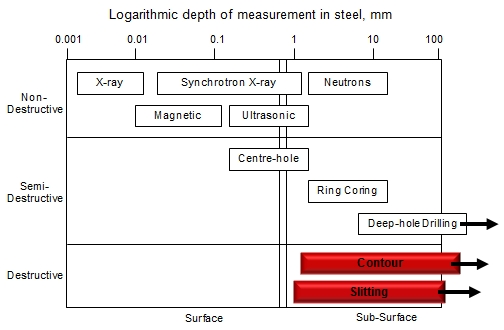
\includegraphics[scale=0.80]{Images/rs_measure}
	\decoRule
	\caption[Non-exhaustive list of residual stresses measurement methods.]{Non-exhaustive list of residual stresses measurement methods (from Hosseinzadeh \parencite{Openuni}).}
	\label{fig:rs_measure}
\end{figure}

A common semi-destructive method is the center-hole drilling. A strain gauge rosette is arranged around a circular area with a diameter of a couple millimetres on a part face. In this area is progressively drilled a shallow cylindrical hole, increment by increment. The new surfaces formed enable the surrounding material to relax, deforming the hole. The strain gauges note this deformation for each increment. By using the ASTM E837-13a standard \cite{ASTM}, those distortions enable us to calculate the residual stresses present in the area before drilling. This method displays practical advantages, such as its speed, versatility in term of materials and its ability to do on-site measurements \cite{G2MT}. \\

A fairly recent destructive technique is the contour method. Developed in the early 2000s by Los Alamos National Laboratory \cite{LANL}.The first step, which makes this technique destructive, requires to cut the part in two. The final result of the method will be the 2D distribution of residual stresses on the cross-section we just obtained. This new free surface will enable the material to deform and relax some of its stresses. The "contour", or shape, of this distorted surface is then measured, by using, for example, a Coordinate Measuring Machine. Then comes the analytical part: a 3D finite-element model of the undeformed cut part is realised. The strain opposite to the one measured with the CMM is then applied to this model as a boundary condition, as if we forced the deformed surface back flat. Processing the finite-element results finally gives the stress distribution of the cross section.\\

Even though many process parameters influence the amount of residual stresses in the cooled part, reliable quantitative relations are difficult to obtain. On top of that, phenomena specific to the material used, such as the formation of precipitates or allotropic transformations, restrain us from applying what is known about the process from one material to another. However, the parameter with the most obvious consequences on residual stresses is the powder bed preheating. While it indeed reduces the thermal gradient around the melt pool, and thus reduces internal stresses as well, it is suggested that the lower yield strength at higher temperature is the strongest stress-reducing effect \cite{Vrancken2016}. \\

Another parameter altering the macroscopic thermal gradient of the part is the presence of building supports, depending on their ability to conduct heat to the platform. Indeed, a part built atop a solid support, or directly onto the building platform has an heat exchange area equal to its section, whereas a honeycomb or another type of hollow support would reduce this area, because the unmelted powder has a much lower heat transfer coefficient\cite{Hodge2014}. Heat generated by the laser would thus escape more slowly out of the part, leading to a higher thermal gradient and, in turn, higher residual stresses \cite{Salmi2017}, as it is shown in Fig. \ref{fig:rs_support}.\\

\begin{figure}[ht]
	\centering
	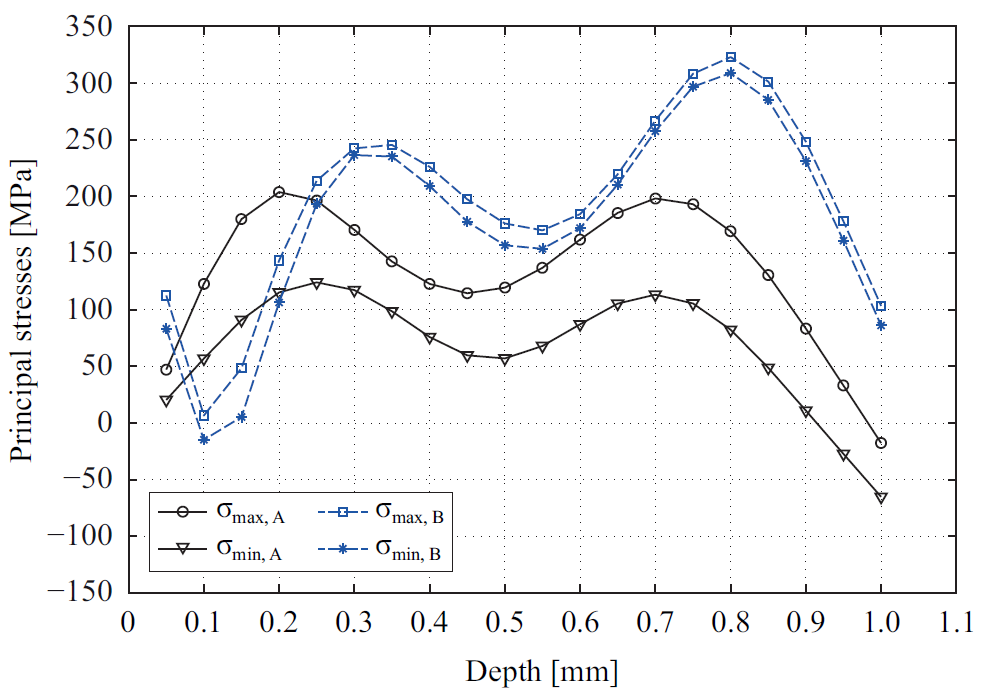
\includegraphics[scale=0.50]{Images/Rs-support}
	\decoRule
	\caption[Principal residual stresses as a function of the depth relative to the surface. Sample B is built onto an undefined hollow support, while A is not]{Principal residual stresses as a function of the depth relative to the surface. Sample B is built onto an undefined hollow support, while A is not (from Salmi et al., 2017 \parencite{Salmi2017}).}
	\label{fig:rs_support}
\end{figure}

\section{Post treatments}
\textcolor{red}{Post-traitements habituels en SLM à expliquer: Shot peening, HIP,... dont traitements thermiques, sur lesquels on se focalise. Expliquer + Propriétés mécas après les traitements}

\textcolor{red}{Source que tu peux utiliser:}

\textcolor{red}{Trevisan et al, ‘On the Selective Laser Melting (SLM) of the AlSi10Mg Alloy: Process, Microstructure, and Mechanical Properties’ (AlSi10Mg de manière générale)}

Effet sur microstructure et dureté:
http://sci-hub.tw/https://link.springer.com/article/10.1007/s11661-015-2980-7

\textcolor{red}{Anne Mertens: 250 deg/2h
https://orbi.uliege.be/bitstream/2268/185421/1/2015-SFFS-Mertens.pdf}

\textcolor{red}{Traitement T6 \parencite{ABOULKHAIR2016139}}

\textcolor{red}{http://sci-hub.tw/https://www.sciencedirect.com/science/article/pii/S0921509316304890}\\

Impact sur fatigue:
https://www.sciencedirect.com/science/article/pii/S0264127516306426

Plein de données de littérature
http://sci-hub.tw/https://www.sciencedirect.com/science/article/pii/S0142112316301463

Unfortunately, although they can be attenuated, as we discussed above, the presence of residual stresses after the fabrication seems unavoidable. However, cast alloys have known the same problems for their whole history. Various treatments have thus been developed over the years to try to reduce and modify these stresses after the initial manufacturing process.

%Recherches biblio....
%\section{Comment référencer?}
%The \code{biblatex} package is used to format the bibliography and inserts references such as this one \parencite{Reference1}. The options used in the \file{main.tex} file mean that the in-text citations of references are formatted with the author(s) listed with the date of the publication. Multiple references are separated by semicolons (e.g. \parencite{Reference2, Reference1}) and references with more than three authors only show the first author with \emph{et al.} indicating there are more authors (e.g. \parencite{Reference3}). This is done automatically for you. %To see how you use references, have a look at the \file{Chapter1.tex} source file. Many reference managers allow you to simply drag the reference into the document as you type.
%
%Scientific references should come \emph{before} the punctuation mark if there is one (such as a comma or period). The same goes for footnotes\footnote{Such as this footnote, here down at the bottom of the page.}. You can change this but the most important thing is to keep the convention consistent throughout the thesis. Footnotes themselves should be full, descriptive sentences (beginning with a capital letter and ending with a full stop). The APA6 states: \enquote{Footnote numbers should be superscripted, [...], following any punctuation mark except a dash.} The Chicago manual of style states: \enquote{A note number should be placed at the end of a sentence or clause. The number follows any punctuation mark except the dash, which it precedes. It follows a closing parenthesis.}
%
%The bibliography is typeset with references listed in alphabetical order by the first author's last name. This is similar to the APA referencing style. To see how \LaTeX{} typesets the bibliography, have a look at the very end of this document (or just click on the reference number links in in-text citations).

\chapter{Materials and methods}
\label{Chap3}
\section{Powder follow-up}

To avoid wasting too much powder, the non-sintered powder remaining in the store after the fabrication process was collected in standard recipients, in order to be recycled and reused. The evolution of its composition and granulometry was monitored during the years to assess its influence on the process and properties.

\subsection{Sieving}

The powder collected from the printer after the process systematically goes through a sieving step, with the aim of limiting the size of the particles used for the next batch. \textcolor{red}{Infos sur la machine?}

\subsection{Grain size and distribution}

For several manufacturing batches along the year, samples of the powder placed inside the store were taken. Those samples were used to conduct composition, which will be discussed just after, and granulometric analyses. \textcolor{red}{Infos sur le procédé? \% en nombre ou en volume?} Four consecutive measures were made for each sample. Four additional measures were taken after the powder was exposed to ultrasonic vibrations, with the aim of breaking agglomerates. 

\subsection{Composition}
%\subsection{Drying}

The composition of several samples of fresh and recycled powder was estimated through inductively coupled plasma (ICP) spectrometry. 

\section{SLM manufacturing}
\label{MMFPP}
The same direct metal printer (DMP) was used to fabricate all specimens throughout this work. It is a \textit{ProX DMP 200} printer, manufactured by \textit{3D Systems} (see figure \ref{fig:Printer}). It uses a laser with a theoretical maximal power of 300 [W] and wavelength $\lambda$ = 1070 [nm] \parencite{3D}. Its actual maximal power is $P_{max}=273.6 [W]$. The maximal envelope capacity of the machine (W x D x H) is 140 x 140 x 125 [mm]. Its typical accuracy is +/- 50 [$\mu m$] for small parts and +/- 0.2\% for large parts. It allows for the set-up of a protection atmosphere. However, it does not integrate any heating feature for the build bed.\\

\begin{figure}[ht]
\centering
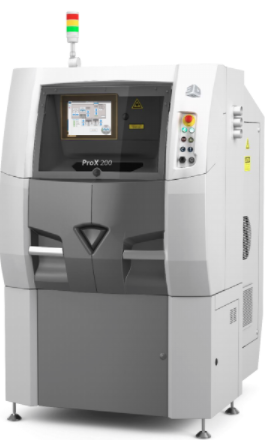
\includegraphics[scale=0.7]{Images/Printer}
\decoRule
\caption[ProX DMP 200 printer]{ProX DMP 200 printer (from the user's ProX DMP 200 general instructions document).}
\label{fig:Printer}
\end{figure}

In this thesis, argon was used as shielding gas. The composition of the gas environment was monitored so as to keep $p_{O2}$ < 500 [ppm]. Laser compensations were set to take into account the excess energy at the start and end of the scanning vectors (see figure \ref{fig:Compens}). These were chosen in accordance with the manufacturer recommendations (figure \ref{fig:Compens1}). The 99\% contour spot size $\phi_{99\%}$ was set to 75 [$\mu m$]. Values for hatch space (h) and layer thickness (t) were respectively set to 100 [$\mu m$] and 30 [$\mu m$]. The scan speed ($v_s$) and the laser power (P) were varied in the ranges [900 ; 1500] [$\frac{mm}{s}$] and [$0.75 \cdot P_{max}$ ; $P_{max}$] respectively, in order to optimise of the built specimens (see section \ref{Rparaopti}). Educated guesses were made based on literature and previous works done at the UCL. The parameters used are resumed in appendix \ref{ppa}. Batches were named in the format X200-\textit{yymmdd}. The prefix "X200" refers to the DMP used. It is followed by the date of printing (6 digits). Recycled powder was used for every batch except for X200-180222 and X200-180228. Figures with detailed specimens positions, denominations, scanning orders and sintering durations for all batches are available in appendix \ref{mda}.\\

\begin{figure}[ht]
\centering
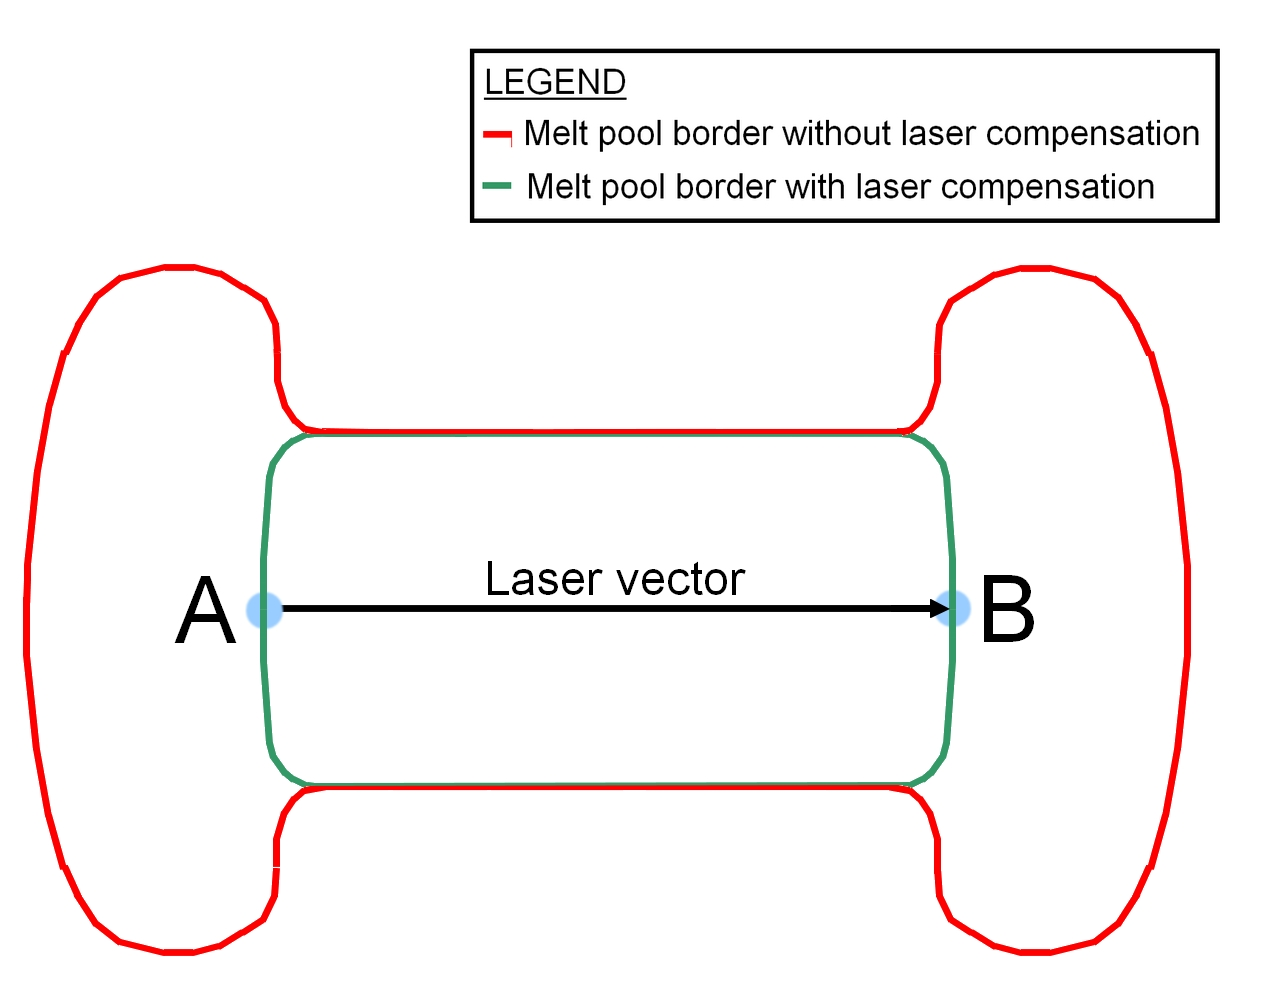
\includegraphics[scale=0.3]{Images/Compens}
\decoRule
\caption[Melt pool contours with and without laser compensation (exaggeration)]{Melt pool contours with and without laser compensation (exaggeration).}
\label{fig:Compens}
\end{figure}

\begin{figure}[ht]
\centering
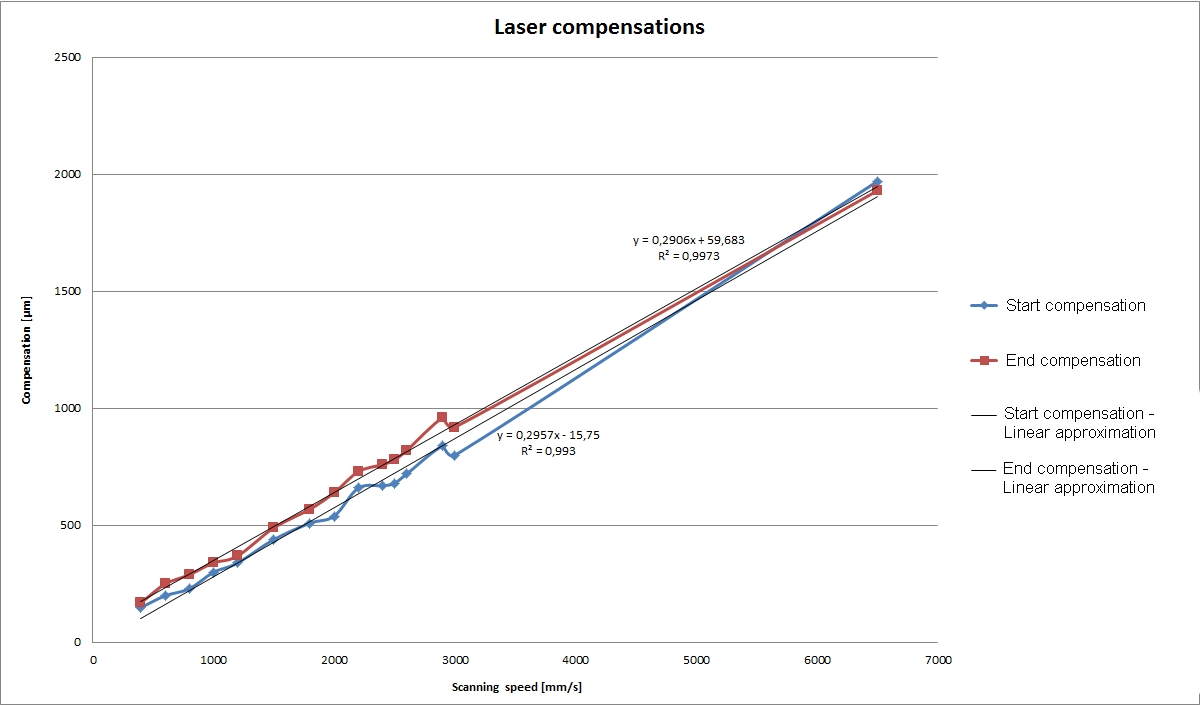
\includegraphics[scale=0.45]{Images/Compens1}
\decoRule
\caption[Laser compensations as a function of the scanning speed (as recommended by the manufacturer)]{Laser compensations as a function of the scanning speed (as recommended by the manufacturer).}
\label{fig:Compens1}
\end{figure}

The batches were first prepared on \textit{DMP ProX Manufacturing}, a dedicated CAD software. It enabled to select the values for the parameters previously mentioned, as well as the position of the specimens. Each specimen was fabricated on building supports. After the completion of the process, they were separated from the plate through electro-erosion. \\

For this thesis, all cylinders and tensile specimens were fabricated vertically. The dimensions notations for the samples types and the tensile specimens detailed geometry are gathered on figure \ref{fig:cc}.\\

\begin{figure}[ht]
\centering
\noindent\makebox[\textwidth]{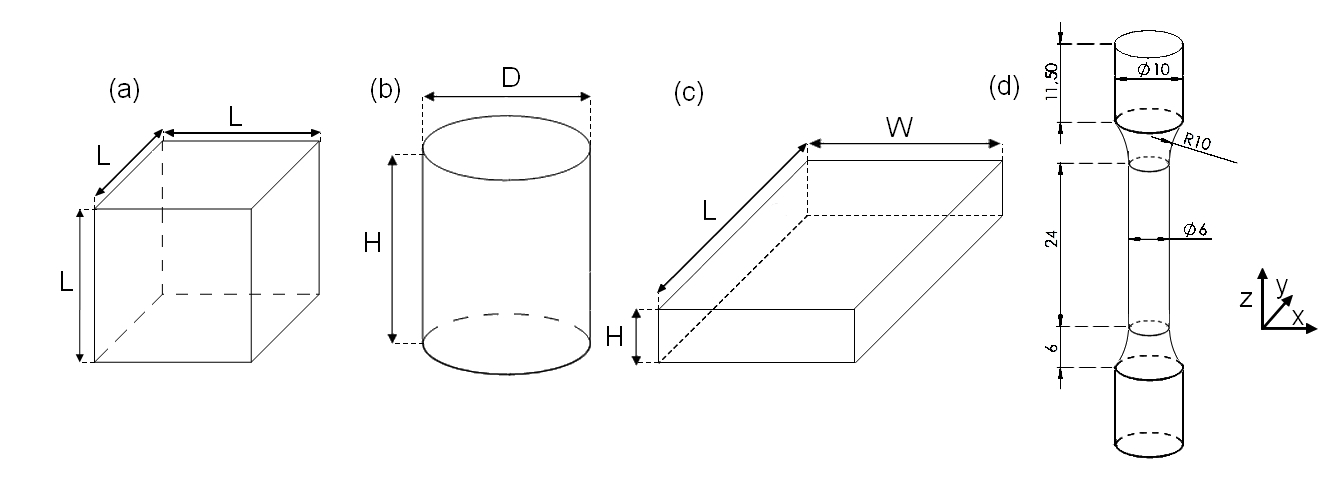
\includegraphics[scale=0.52]{Images/cc}}
\decoRule
\caption[Dimensions notations for (a) cubic specimens (b) cylindrical specimens (c) parallelepiped specimens (d) tensile specimen]{Dimensions notations for (a) cubic specimens (b) cylindrical specimens (c) parallelepiped specimens (d) tensile specimens with dimensions in [mm]}
\label{fig:cc}
\end{figure}


An island scanning strategy was chosen on account of research done on the subject (see section \ref{pp}). It is a hexagonal pattern. The replicated hexagon's smallest width is equal to 5 [mm]. An overlap of 100 [$\mu m$] was set, as illustrated on figure \ref{fig:OL}. There is a rotation of $90^\circ$ and a translation of a third of basis vector between two successive powder layers as depicted by figure \ref{fig:Lassup}. In the case of a contour scanning strategy, the contours were pre scanned for each powder layer with the same P and $v_s$ used for the bulk (see figure \ref{fig:LasCSC}). The scanning order among the samples was automatically chosen. \\

\begin{figure}[ht]
\centering
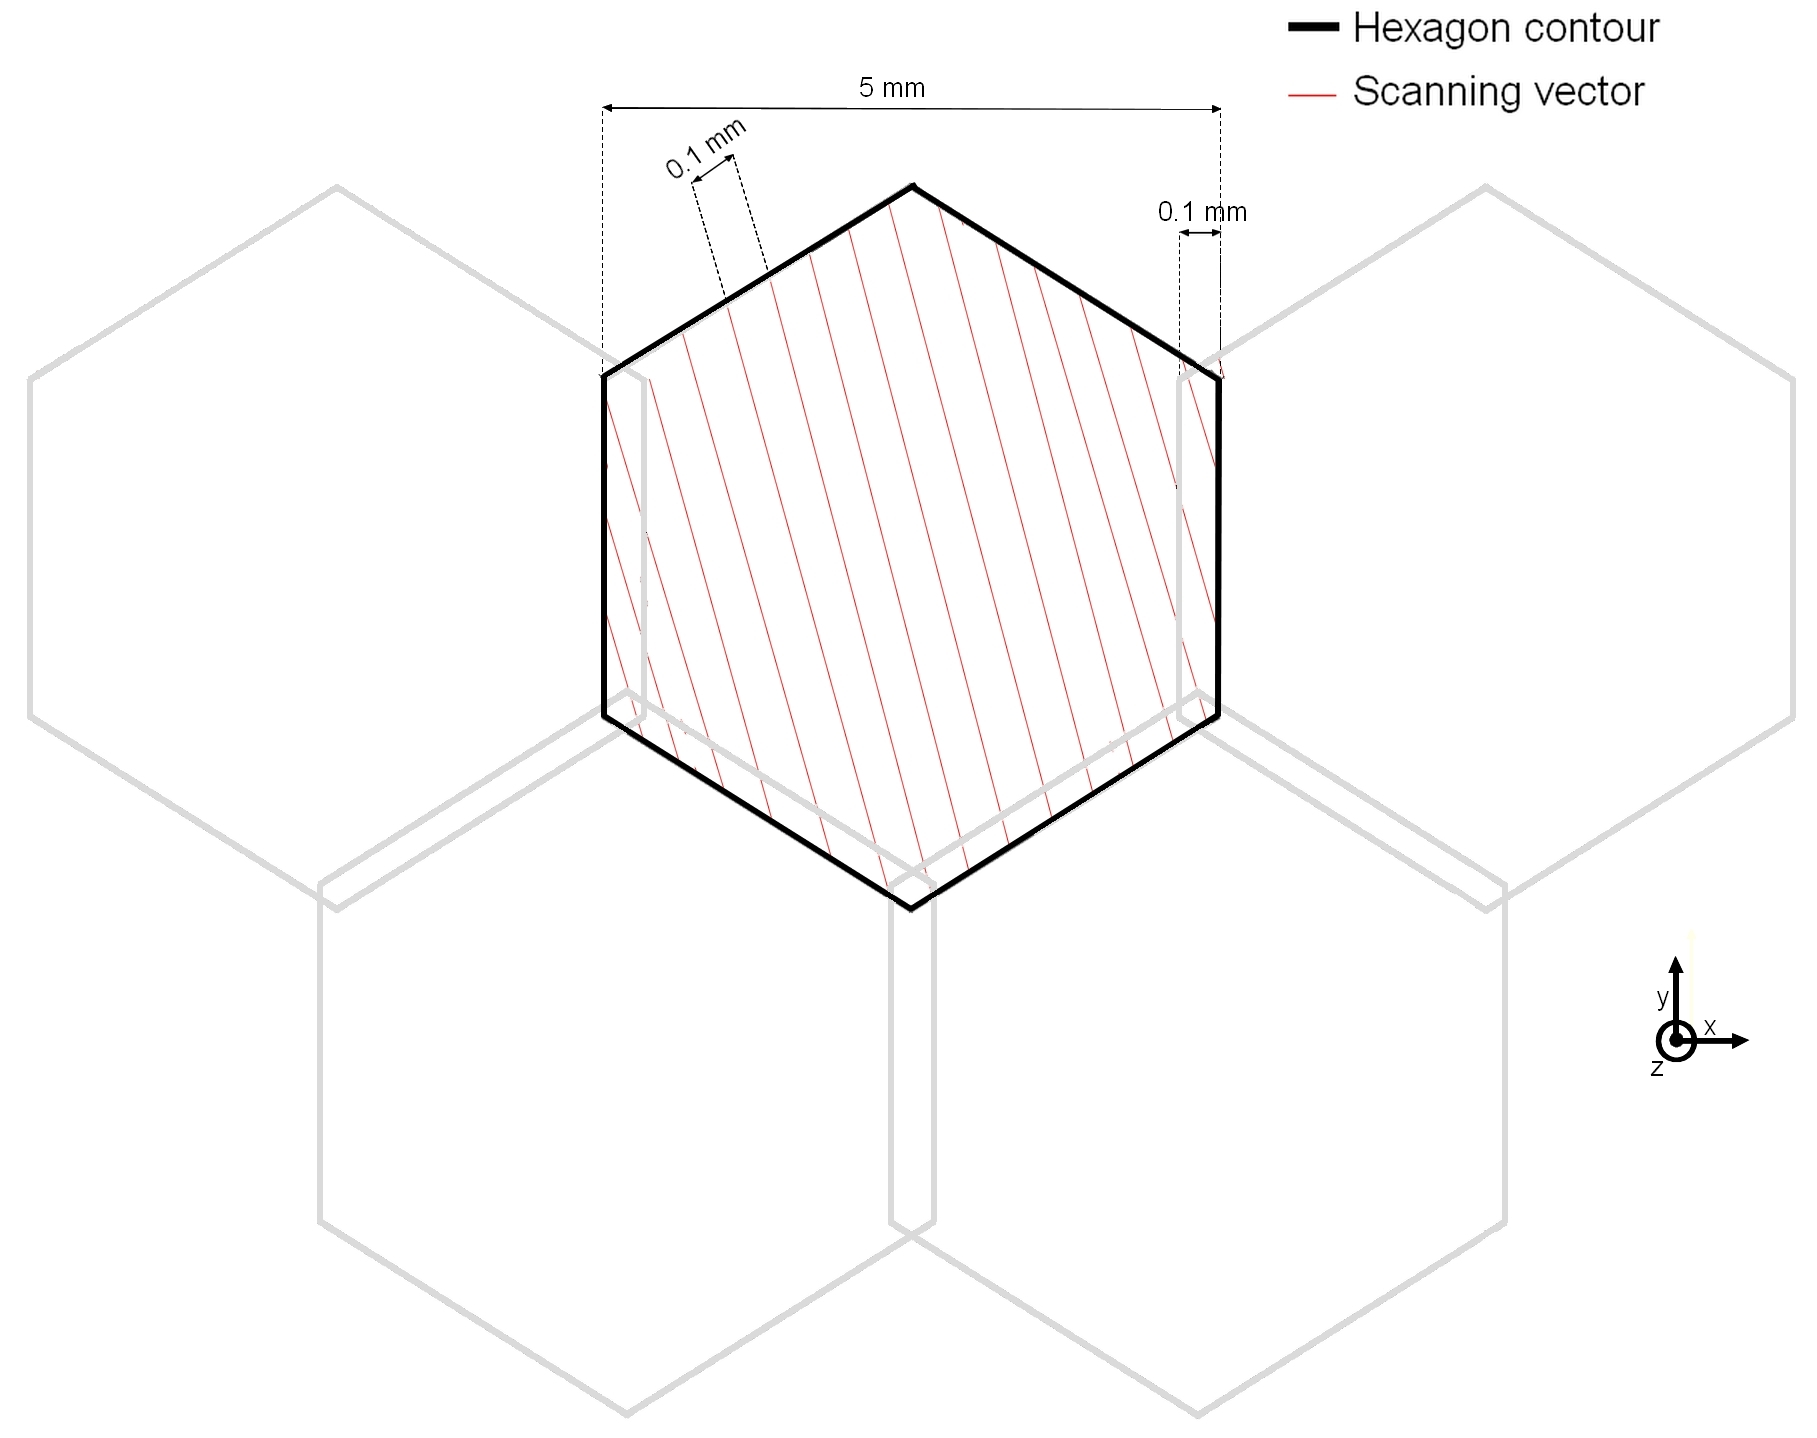
\includegraphics[scale=0.27]{Images/OL}
\decoRule
\caption[Schematic representation of the hexagonal pattern scanning strategy]{Schematic representation of the hexagonal pattern scanning strategy}
\label{fig:OL}
\end{figure}

\begin{figure}[ht]
\centering
\noindent\makebox[\textwidth]{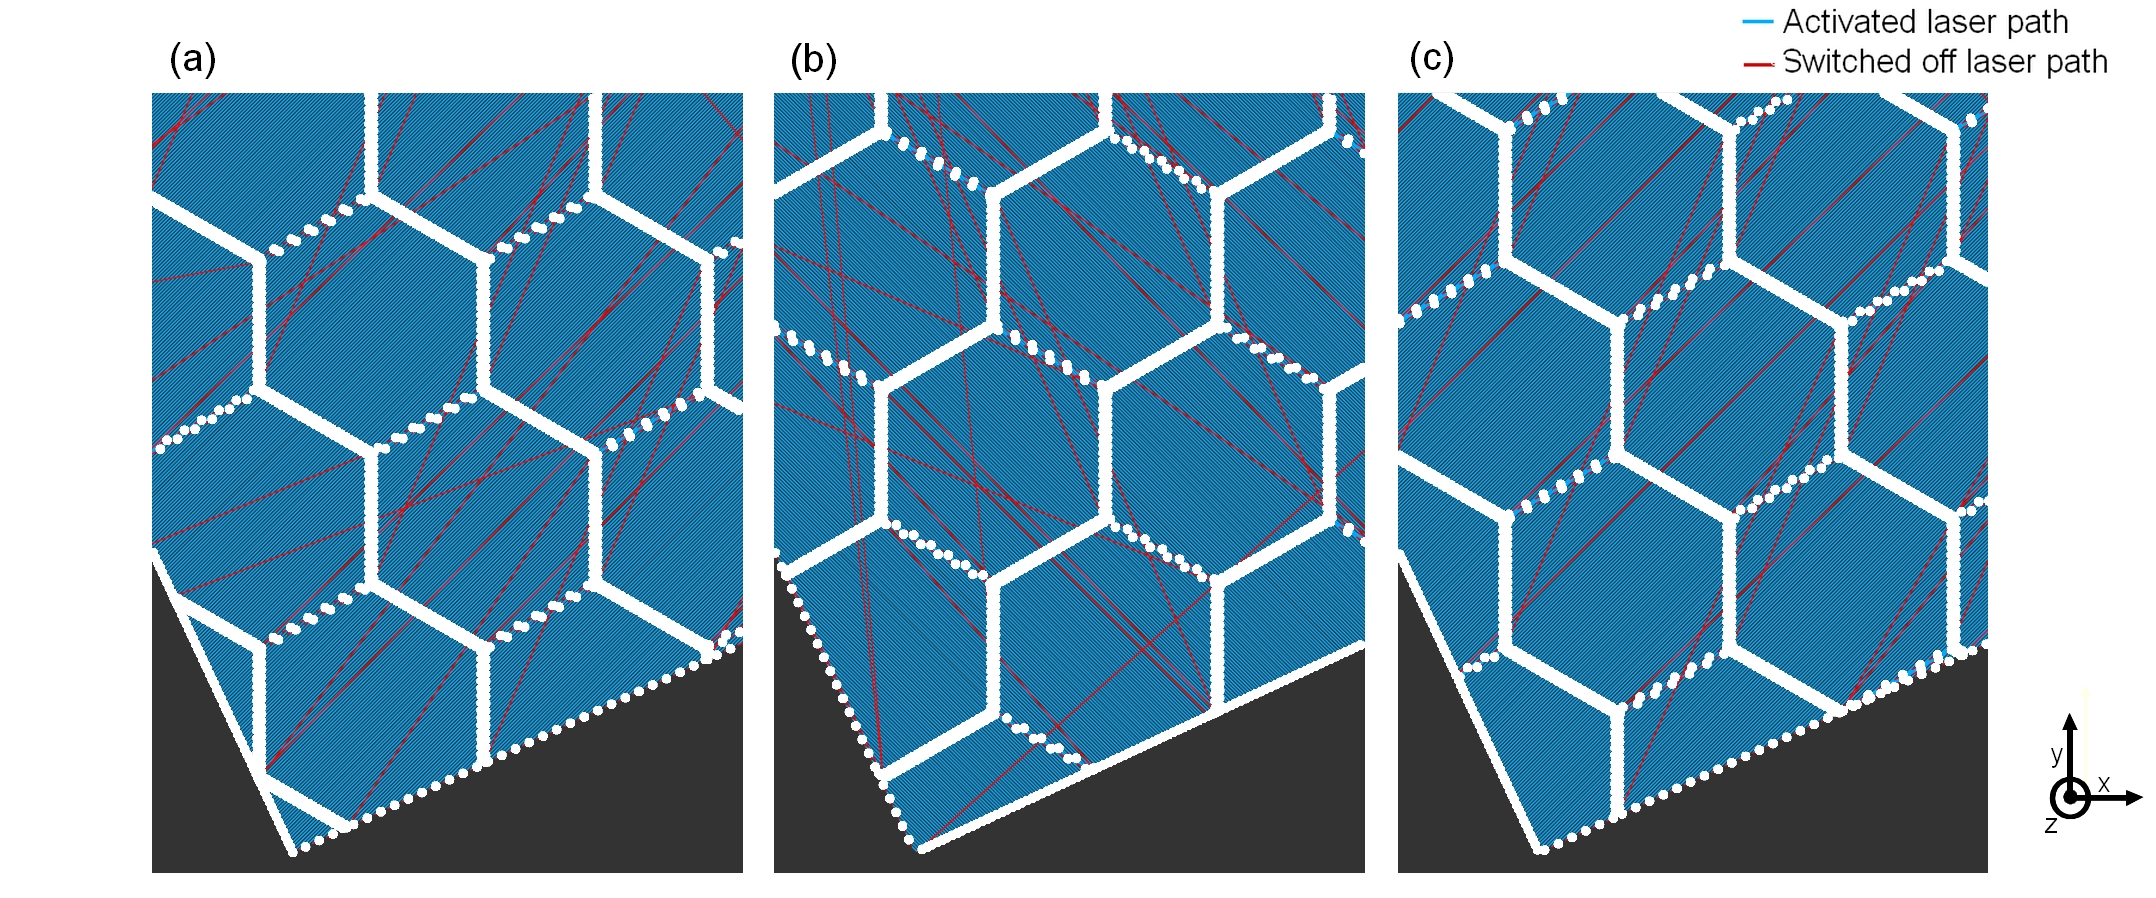
\includegraphics[scale=0.3]{Images/Lassup}}
\decoRule
\caption[Screen capture of the laser scanning pattern for a parallelepiped sample: (a) Layer $n$ (b) Layer $n+1$ (c) Layer $n+2$]{Laser scanning pattern for a parallelepiped sample: (a) Layer $n$ (b) Layer $n+1$ (c) Layer $n+2$}
\label{fig:Lassup}
\end{figure}

\begin{figure}[ht]
\centering
\noindent\makebox[\textwidth]{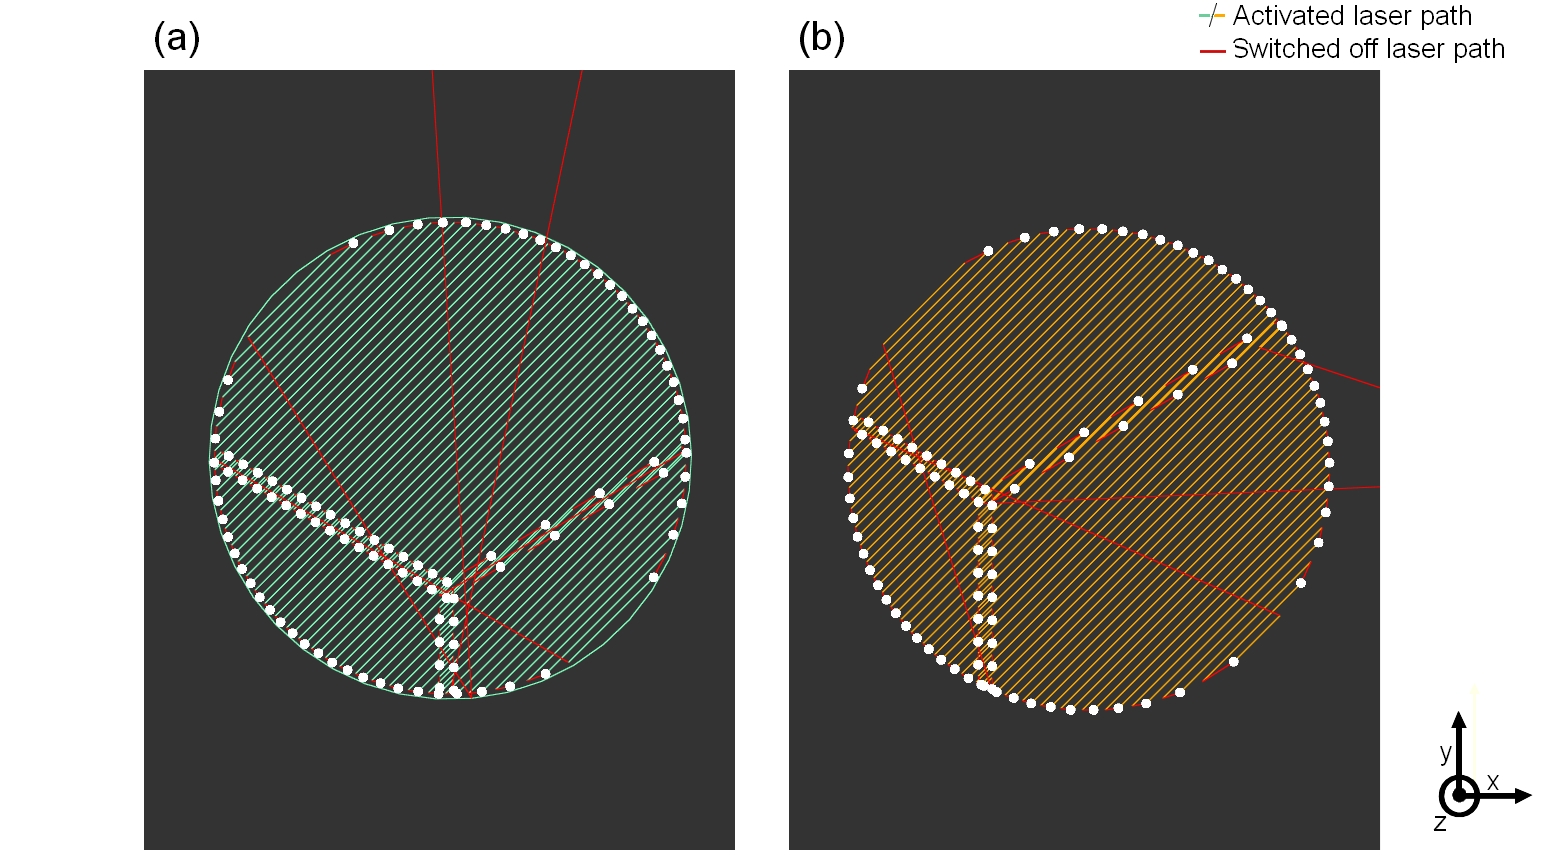
\includegraphics[scale=0.4]{Images/LasCSC}}
\decoRule
\caption[Screen capture of the laser path for a cylindric sample (a) with contour scanning strategy (b) without contour scanning strategy]{Screen capture of the laser path for a cylindric sample (a) with contour scanning strategy (b) without contour scanning strategy}
\label{fig:LasCSC}
\end{figure}

\section{Heat treatments}
\label{MMHT}
The heat treatments were conducted inside a unique oven of the VT 5050 EKP model, manufactured by Heraeus, which is able to reach a temperature of 400$^\circ$ C. The samples were introduced in the cold oven, under an air atmosphere, and after the annealing, were left to cool down in the turned off oven, with the door opened. Samples temperature data was obtained through a T-type thermocouple arc-welded to the sample surface, thanks to a \textit{Labfacility L60 Thermocouple \& Fine Wire Welder}. \textcolor{gray}{[Méthode de soudage, élévation de la température durant l'opération]} The data was displayed and saved every 10 seconds, with a precision of 0.1$^\circ$ C, thanks to a \textit{Agilent 34972A LXI Data Acquisition/Switching Unit}, connected to the thermocouple (see Fig.\ref{fig:agilent} for both devices). For reasons that can not be explained only by thermal inertia, setting the oven to the target temperature was not efficient to heat the specimens to the same temperature. After a couple of tests, the oven was then set at a temperature about 20$^\circ$ C above the target, so that the temperature measured by the thermocouple welded on the sample reached the target temperature.\\

\begin{figure}[ht]
	\centering
	\includegraphics[scale=0.30]{Images/agilent}
	\decoRule
	\caption[(a) \textit{Labfacility L60 Thermocouple \& Fine Wire Welder} and (b) \textit{Agilent 34972A LXI Data Acquisition/Switching Unit}.]{(a) \textit{Labfacility L60 Thermocouple \& Fine Wire Welder} and (b) \textit{Agilent 34972A LXI Data Acquisition/Switching Unit}.}
	\label{fig:agilent}
\end{figure}

Due to the inaccuracy of the oven, maintaining the samples at the exact target temperature was not possible. The holding plateaus were thus rather slow increasing slopes. For most of the samples, the theoretical beginning of the holding was set when the specimen reached a temperature 5$^\circ$ C below the target value, so that the sample average temperature for the complete holding was the closest possible to target value. A representative heating curve is available in Fig. \ref{fig:TT250-2-curve}. By posterior calculations, it appeared that all the samples have been heated at an approximative rate of 6$^\circ$C/min. The non-linearity of cooling prevents us to give overall rate, but during the 20 minutes, the specimens cool down by about 7$^\circ$C/min. \\

\begin{figure}[ht]
	\centering
	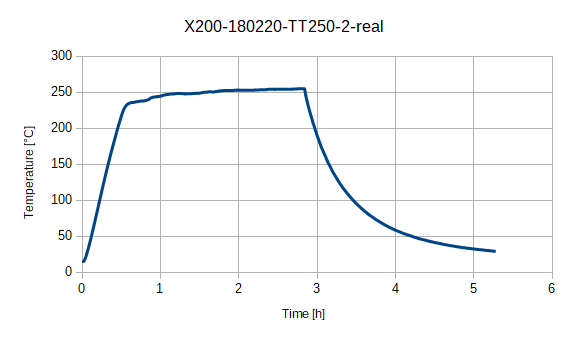
\includegraphics[scale=0.70]{Images/X200-180220-TT250-2-real}
	\decoRule
	\caption[Temperature curve measured by the T-type thermocouple for the cubic sample annealed at 250$^\circ$C for 2 hours.]{Temperature curve measured by the T-type thermocouple for the cubic sample annealed at 250$^\circ$C for 2 hours.}
	\label{fig:TT250-2-curve}
\end{figure}

Samples that were subject to a heat treatment were named in a particular format, to ease distinction between them. They received the name of the batch, followed by "TT-\textit{holdingtemperature-holdingtime-specificities}". Cubes that were subject to heat treatments were 5 x 5 x 5 [mm$^3$].\\

%\begin{figure}[ht]
%	\centering
%	\includegraphics[scale=0.7]{Images/HTdevices}
%	\decoRule
%	\caption[ProX DMP 200 printer]{ProX DMP 200 printer (from the user's ProX DMP 200 general instructions document).}
%	\label{fig:HTdevices}
%\end{figure}

The main objective of most of the research about aluminium alloys AM is to obtain parts with properties at least as good as their conventional cast counterparts. To obtain a larger panel of properties, a vast number of heat treatments have been developed for die cast alloys. The classical treatment of stress-relief for aluminium consists of a heating up to 300$^\circ$ C, with a holding of 2 hours, followed by a slow cooling \cite{Mertens170406}. This treatment, and variations around him, have been tried on a number of additively manufactured samples, in order to assess their effect on the microstructure and mechanical properties of the parts.\\

A first series of cubic samples was manufactured using the optimised process parameters from Section \ref{Rparaopti}, namely ($P=75\% P_{max}$ ; $v_s=1200 [\frac{mm}{sec}]$ ; $E_d=57 [\frac{J}{mm^3}]$) and a different heat treatment was applied to each one of them. The complete list of cubes treated can be found in Table \ref{tab:RTT}.\\

\begin{center}
\begin{table}[ht]
\noindent\makebox[\textwidth]{\begin{tabular}{|c|c|c|c|}
	\hline 
	Specimen & Holding time [min] & Aimed holding temp. [$^\circ$C] & Max. temp. [$^\circ$C] \\ 
	\hline 
	X200-180220-TT150-2 & 120 & 150 & - \\ 
	\hline 
	X200-180220-TT200-2 & 120 & 200 & - \\ 
	\hline 
	X200-180220-TT300-2 & 120 & 300 & 256 \\ 
	\hline 
	X200-180220-TT300-2-plaque & 120 & 300 & 281 \\ 
	\hline 
	X200-180220-TT150-2-real & 120 & 150 & 156 \\ 
	\hline 
	X200-180220-TT200-2-real & 120 &200  & 203 \\ 
	\hline 
	X200-180220-TT250-2-real & 120 & 250 & 255 \\ 
	\hline 
	X200-180220-TT300-2-real & 120 & 300 & 302 \\ 
	\hline 
	X200-180220-TT300-1-real & 60 & 300 & 302 \\ 
	\hline 
	X200-180220-TT360-1-real & 60 & 360 & 371 \\ 
	\hline 
	X200-180220-TT300-5m-real & 5 & 300 & 300 \\ 
	\hline 
	X200-180319-TT225-2-real & 120 & 225 & 242 \\ 
	\hline 
\end{tabular}} 

\caption[List of the cubic heat-treated specimens]{List of the cubic heat-treated specimens}
\label{tab:RTT}
\end{table}
\end{center}


\section{Characterisation}

\subsection{Density}

\subsubsection{Hydrostatic weighing}

Multiple methods were considered to estimate the relative density of the fabricated specimens. The first one is hydrostatic weighting (HW), or hydrodensitometry. It is a direct application of the well-known Archimedes' principle, which can be stated as follows: " When a body is (partially or totally) immersed in a fluid, the upthrust on the body is equal to the weight of fluid displaced." \parencite{ADictionaryofPhysics}. By weighing each pieces in air and in water - giving respectively values of dry weight $W_a$ and underwater weight $W_w$ - one can calculate the apparent density $\rho_a$ \parencite{MethArch}:

$$\rho_a=\frac{W_a}{W_a-W_w} \cdot \rho_w $$

where $\rho_w$ is the water density. The apparent relative density $\rho_{a,rel}$ of the specimens can then be calculated with:

$$\rho_{a,rel} = \frac{\rho_a}{\rho_b} $$

where $\rho_b = 2.68 [\frac{g}{mm^3}]$ is the theoretical bulk density of AlSi10Mg \parencite{Bulk}. All weightings were done with a \textit{Sartorius BP121S} analytical balance with precision of 0.1 [mg] \parencite{Balance}. Samples were immersed in demineralised water for more than twelve hours before the measurements to impregnate them. The weightings were also done in demineralised water. Water temperature was measured with a precision glass thermometer to compute $\rho_w$ as accurately as possible thanks to tabulated values \parencite{Eau}. Multiple measurements were done for each sample in order to increase the method's reliability. \\

The technique was employed with "as-built" and polished cubes. For this second option, all six faces of the tested cubes were polished with P320 silicon carbide sandpaper sheets and briefly with P1200 ones. In most cases, the tests were done with samples of volumes $\simeq 1 [cm^3]$ and weights $\simeq 2.5 [g]$.\\

\subsubsection{Relative optical density image analysis}

Another method was used to estimate the relative density of the various samples: the relative optical density image analysis (RODIA). For this purpose, the samples were cut with a micro-cutting machine and underwent the polishing routine detailed in table \ref{tab:pol}. Pictures of the polished sections were then taken under the optical microscope. An \textit{Olympus AX70} microscope was used, with 5x and 10x magnification. The pictures were taken with a smart-phone through the lens of the microscope. The used camera has a resolution of 16 [MP]. A camera is directly connected to the microscope at the laboratory, but it only has 5 [MP] resolution. It was thus chosen not to use it. \\

With the help of the \textit{ImageJ} software, the surface of both the porosities and the whole surface could be isolated for each analysed image (see figure \ref{fig:ImageJ}). The surface fraction occupied by porosities could then be obtained as the ratio between the areas of the two (in pixels). If we approximate that the porosities surface fraction is equal to the volumetric one, that method gives an estimation of the relative density $\rho_{rel}$.

\begin{center}
\begin{table}[h]
\noindent\makebox[\textwidth]{\begin{tabular}{|c|c |c |c| c|c|}
    \hline
    Step &  Polishing surface & Abrasive & Grain size & Lubricant type & Rotation speed [rpm]\\

\hline
\hline   
    1 & MD-piano 220 & Diamond & P220 & Water & 200-300 \\
    2 & MD-piano 1200 & Diamond & P1200 & Water & 200-300\\
    3 & MD-largo & DP-spray & 9 $\mu m$ & Alcohol & 150\\    
    4 & DP-DAC & DP-spray & 3 $\mu m$ & Alcohol & 150 \\ 
    5 & DP-NAP & DP-spray & 1 $\mu m$ & Alcohol & 150 \\  
    \hline

\end{tabular}}

\caption[Polishing routine for Al-Si alloys]{Polishing routine for Al-Si alloys}
\label{tab:pol}
\end{table}
\end{center}

\begin{figure}[h]
\centering
\centerline{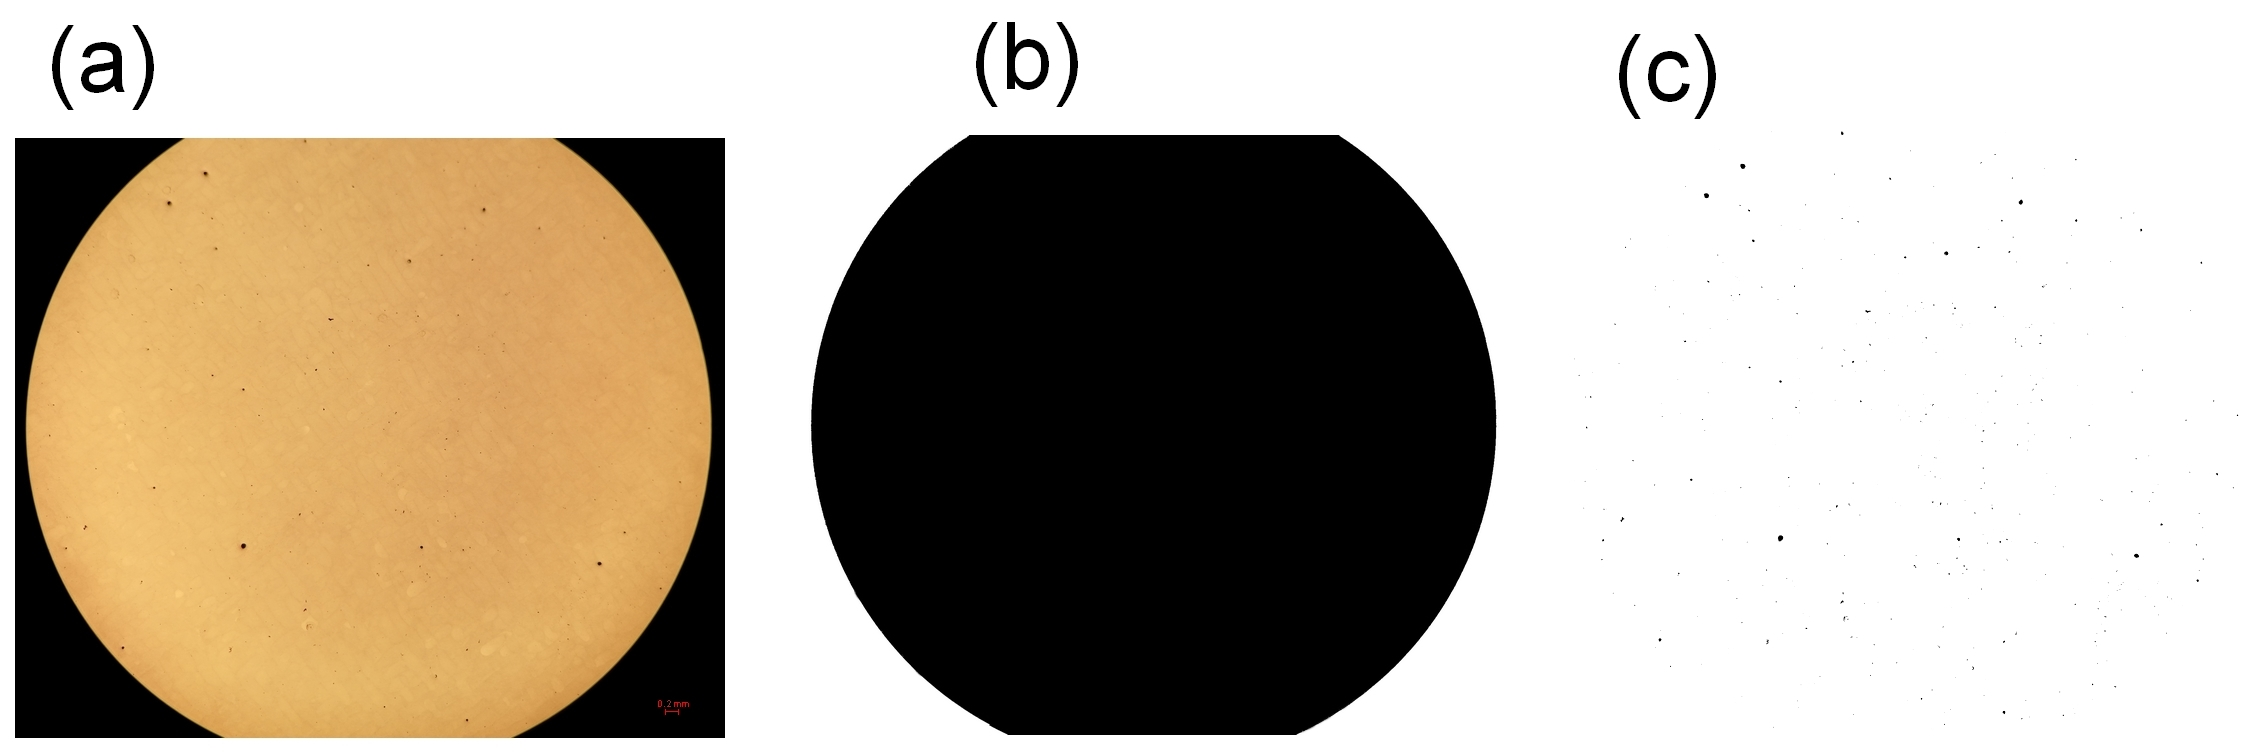
\includegraphics[scale=0.29]{Images/ImageJ-cub1}}
\decoRule
\caption[RODIA procedure for specimen X200-180319-cub 1: (a) Original picture of polished section (b) Whole surface isolation with \textit{ImageJ} (c) Porosities isolation with \textit{ImageJ}.]{RODIA procedure for specimen X200-180319-cub 1: (a) Original picture of polished section (b) Whole surface isolation with \textit{ImageJ} (c) Porosities isolation with \textit{ImageJ}.}
\label{fig:ImageJ}
\end{figure}

The images isolations in "foregrounds" and "backgrounds" were done through manual thresholding based on pixel intensity quantifications.  %https://imagej.net/Thresholding#Global_thresholding
An optimal threshold was sought for porosities isolation so as to include only holes, and as many as possible. Particular attention was given to the photography in order to obtain the best contrast, focus and intensity homogeneity. Between two and five photographs were taken for each specimen to build a representative sample.

\subsection{Microstructure}

\subsubsection{Optical microscopy}
\label{MMOM}
Mesures Taille de bains:


In order to make the identification of the melt pools boundaries possible, the samples underwent the polishing routine detailed in table \ref{tab:pol}. They were then etched with	a Keller's reagent. It is a popular etchant containing hydrochloric acid, hydrofluoric acid and nitric acid diluted in distilled water. [Attaque préférentielle->distinction à l'optique][ + ImageJ] As SLM involves melt pools overlapping to ensure consolidation, one cannot measure the actual original melt pools dimensions. The method has thus only been used   as a tool to compare samples.

Densité
Autre chose?

\subsubsection{Scanning electron microscopy}

Microstructure and fracture surfaces were observed thanks to a XXXXX Scanning Electron Microscope, both with secondary electrons imaging. Microstructure observation required the same polishing routine as for optical microscopy, with of the exception of the last step of etching, which is replaced by a smooth mechano-chemical polishing thanks to an Oxide Polishing Suspension (\textit{Struers Op-S NonDry}).


\subsection{Residual stresses}

Measurements of residuals stresses was performed by ..., in ..., Malta. Two parallelepiped specimens were specifically built to undergo the semi-destructive method of hole drilling. One was tested as-built, while the other was heat-treated at 300$^\circ$C for 2h. Their dimensions are x  x  x [mm$^3$]. Machining \textcolor{gray}{fraisage, pas électro-découpage} of the sample was performed after the eventual heat treatment, removing the least matter possible, before shipping to Malta. Machining was done in order to reduce rugosity on the top and bottom faces of the samples, because smooth surfaces are necessary for the correct fixation of the gauges. \\

From the deformation measured by the strain gauges during the hole drilling, residual stresses were calculated with the integral method, as well as with its simplified approximation \cite{Trebuna08}, the power series method.\\

For the sake of comparison, 5 samples were also subjected to a \textit{Bruker D8 Advance X-Rays Diffractometer}, in order to obtain qualitative information about the deformation of the crystal lattice, and thus, residual stresses. The wavelength of the X-ray was 1.5406 [nm], and the angle was varied between 20 and 100$^\circ$. \\

\subsection{Mechanical properties}

\subsubsection{Hardness test}

Vickers hardness measurements were made with a \textit{Wolpert Dia-Testor 2RC} tester. All analysed specimens were previously cut with a micro-cutting machine. This permitted the testing of the bulk hardnesses of the samples (at least at a few millimetres from the original surfaces). For each test, a pyramidal indenter (see figure \ref{fig:Vick}) was pressed during 10 [sec] onto the material with a load of 10 [kg]. The indentation durations were measured with a digital timer and the tests were stopped manually. The two diagonals lengths of the resulting indents were then evaluated using a ruler on the screen of the machine, which displays the image of the sample's surface that is captured by an embedded optical microscope.\\

\begin{figure}[ht]
\centering
\centerline{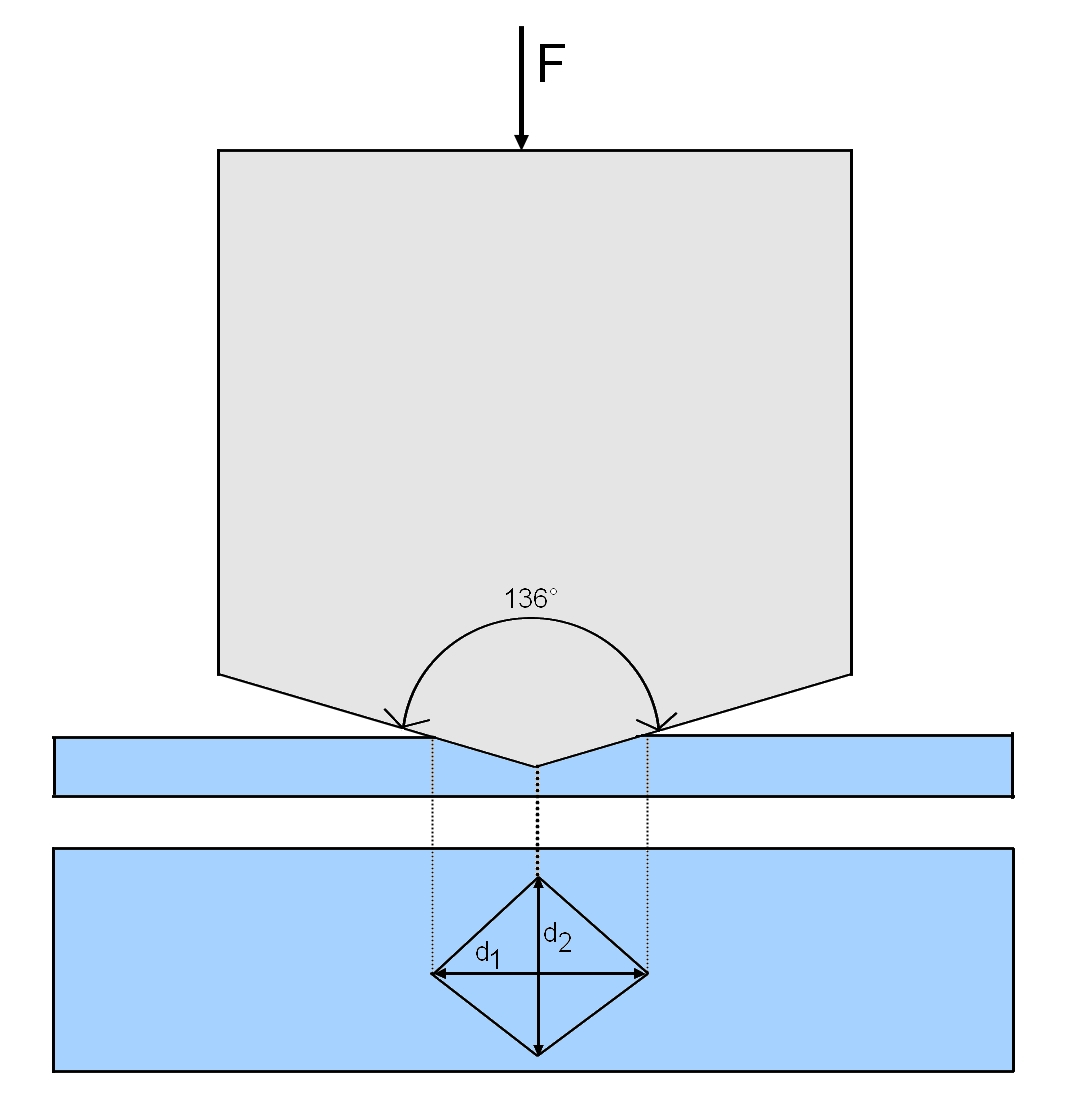
\includegraphics[scale=0.29]{Images/Vickers}}
\decoRule
\caption[Schematic representation of the Vickers hardness test]{Schematic representation of the Vickers hardness test}
\label{fig:Vick}
\end{figure}

Three to ten tests were made for each sample and the mean diagonal length value was computed for every test. The corresponding Vickers hardness values $H_v$ could then be estimated by means of a conversion table (see \ref{AppendixB}).\\

\subsubsection{Tensile tests}
\label{MMTT}
The tensile tests were performed on a \textit{RetroLine testControl II} screw-driven electro-mechanical testing system manufactured by \textit{Zwick Roell}. It works in the following manner:

\begin{itemize}
\item The cylindrical specimen is clamped on its extremities with grips. Both of them are fixed to a cross head (see figure \ref{fig:Trac}).

\item Parameters are selected thanks to a software connected to the machine: 
One must enter the extensometer initial gauge length $L_0$, the cross head speed and the pre load (used to limit the backlash in the assembly). The initial minimal value $d_o$ for the specimen diameter is also measured with a digital calliper and specified in the program.

\item The contact extensometer is placed on the sample. Its purpose is to measure the length change $\Delta L$ during the test. 

\item The lower cross head goes down. This induces a force $F$ and a displacement in the specimen, both of which are saved in an \textit{Excel} file. The test goes on until the fracture of the specimen occurs, unless if it is stopped beforehand.
\end{itemize}

\begin{figure}[ht]
\centering
\centerline{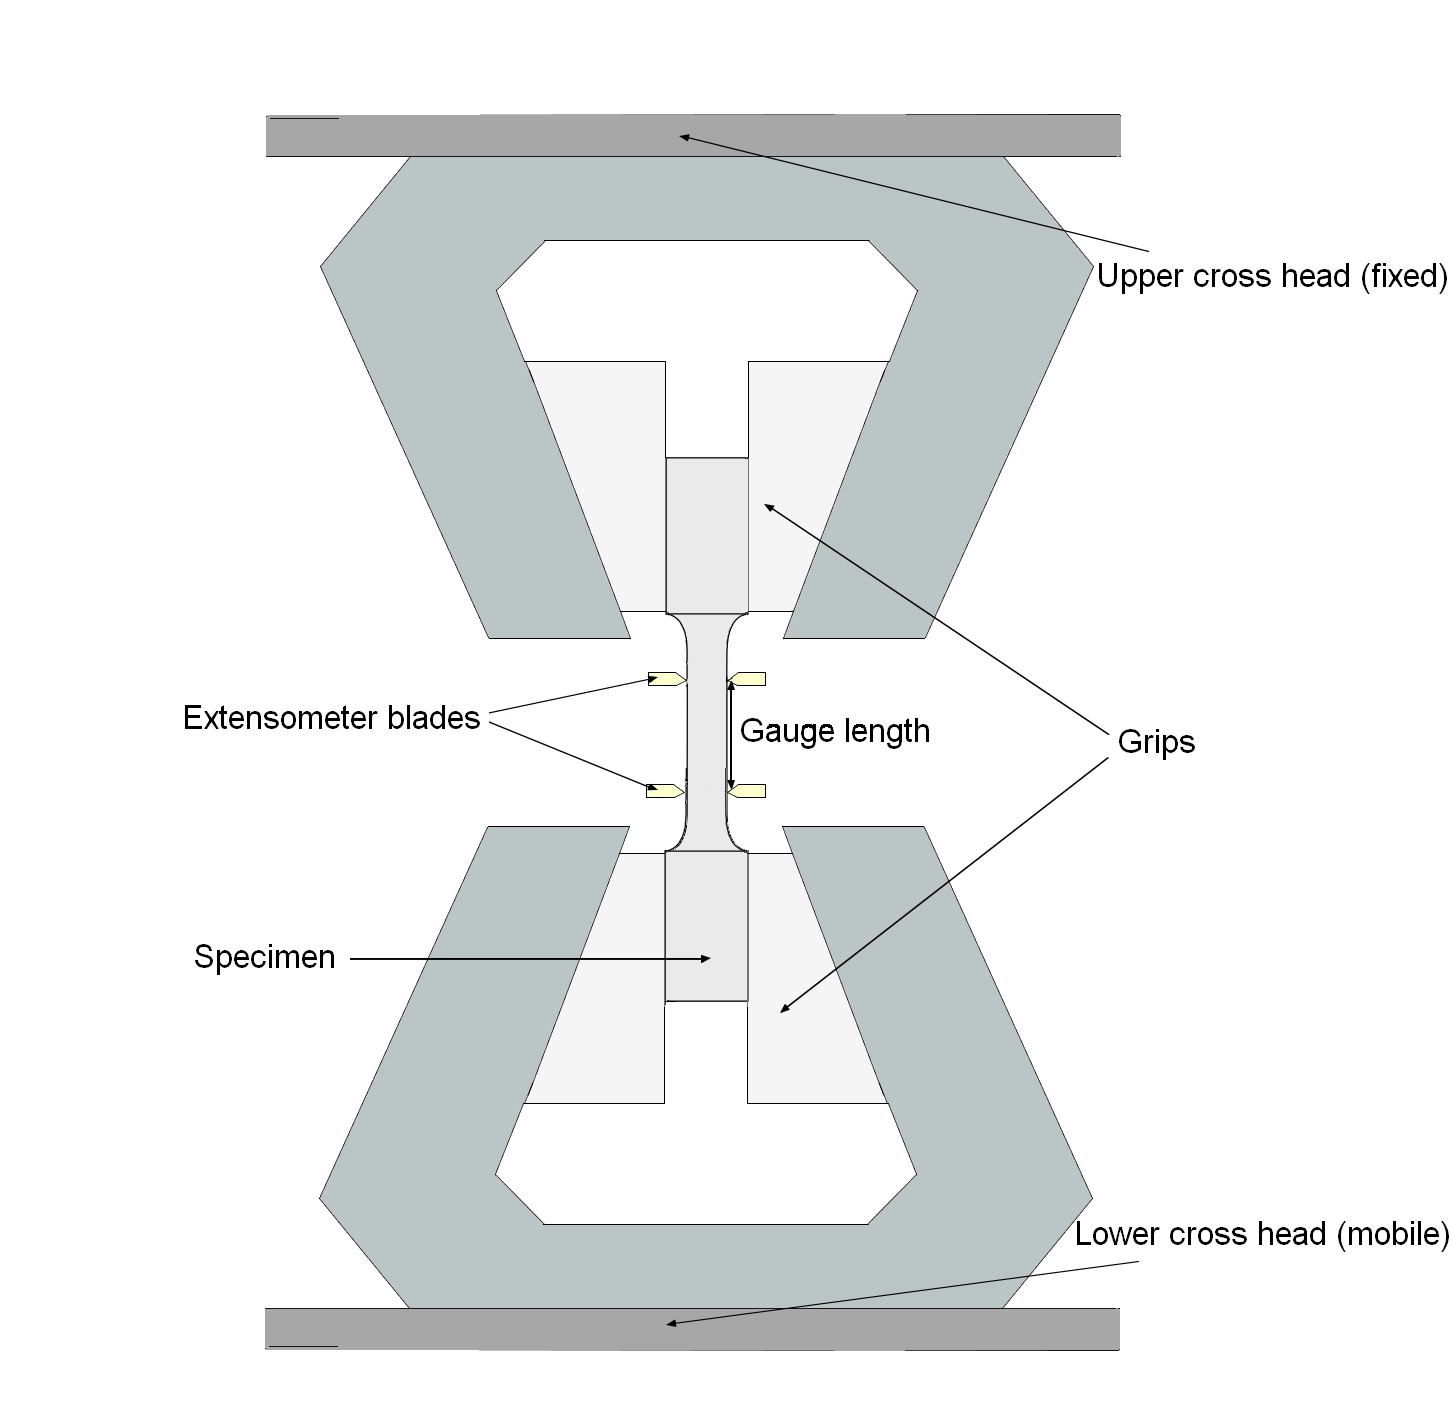
\includegraphics[scale=0.3]{Images/Trac}}
\decoRule
\caption[Schematic representation of the tensile test mounting]{Schematic representation of the tensile test mounting}
\label{fig:Trac}
\end{figure}

The tensile specimens used all originated from batch X200-190417. They were fabricated using the optimised set of parameters: $P=0.75\% P_{max}$ and $v_s=1200 [\frac{mm}{s}]$. Their minimal diameter is equal to 6 [mm]. Further details about their geometry and heat treatments can be consulted respectively in sections \ref{MMFPP} and \ref{MMHT}. For each test, the extensometer gauge length was set to 18 [mm]. This is approximately the maximal possible value, given the short length of the specimens. A pre load of 15 [N] was adopted and a cross head speed of 1 [$\frac{mm}{min}$] was chosen in accordance with what had been done in a previous work at UCL. It was decided to interrupt the tensile tests of one AB specimen and of two others - that underwent heat treatments at 200$^\circ$C and 300$^\circ$C. In that way, the damage mechanisms could be observed afterwards. Table \ref{tab:stoptract} regroups the strain limits at which the tests were stopped. They correspond roughly to the onset of necking.\\

 \begin{center}
\begin{table}[ht]
\noindent\makebox[\textwidth]{\begin{tabular}{|c|c|}
    \hline
    Sample & Strain limit [-] \\
\hline
\hline   
    X200-180417-3 & 0.01\\
    X200-180417-6 & 0.06 \\
    X200-180417-9 & 0.08\\
    \hline

\end{tabular}}

\caption[Strain limits for interrupted tensile tests of batch X200-180417 specimens]{Strain limits for interrupted tensile tests of batch X200-180417 specimens}
\label{tab:stoptract}
\end{table}
 \end{center}

A tensile test can be used to compute multiple properties. First of all,  the engineering stress ($\sigma_{eng}$) and strain  ($\epsilon_{eng}$) were computed at each time step for every tested samples. The formulas below were used:\\

\begin{align*}
\sigma_{eng}=\frac{F}{A_0}=\frac{F}{\frac{\pi d_0^2}{4}}
\end{align*}

\begin{align*}
\epsilon_{eng}=\frac{\Delta L}{L_0}=\frac{L-L_0}{L_0}
\end{align*}

On the basis of the stress-strain curve, the following characteristics could be computed:

\begin{itemize}

\item The Young's modulus E: it is used to characterize the stiffness of a material. The tested specimen first deforms elastically, which corresponds to a linear strain-strain relationship. The slope value for the corresponding part of the curve is  E. It is found via numerical linear regression in the $\epsilon_{eng}$ between 0 and $\simeq 0.1$[\%].

\item The elastic limit $\sigma_y$: it is the $\sigma_{eng}$ at which the plastic strain (non-linear) becomes non negligible. The 0.2 [\%] criterion was used. In this manner, $\sigma_y$ is found as the intersection of the stress-strain curve with the line of slope E passing through point ($\epsilon,\sigma$)=($0.2 [\%],0 [MPa]$).

\item The ultimate tensile strength $\sigma_u$: it is simply the maximal $\sigma_{eng}$ attained during the test.

\item The strain at fracture $\epsilon_{f}$: in the case of fragile fracture, the value of $\epsilon_{eng}$ at the end of the test could be used. However, if the specimen underwent a necking mechanism -  as there is strain localisation - the final $\epsilon$ does not constitute a good approximation. In that case, the specimen final minimal diameter $d_f$ was measured with a profile projector. The true final strain $\epsilon_{f,true}=ln(\frac{L_f}{L_0})$ could then be computed using the volume conservation hypothesis: $$L_0 \cdot A_0 = L_f A_f $$
which implies that $\epsilon_{f,true}=ln(\frac{A_0}{A_f})=ln(\frac{d_0^2}{d_f^2})$. All the properties mentioned above are illustrated in figure \ref{fig:Tract}.


\end{itemize}

 \begin{figure}[ht]
\centering
\centerline{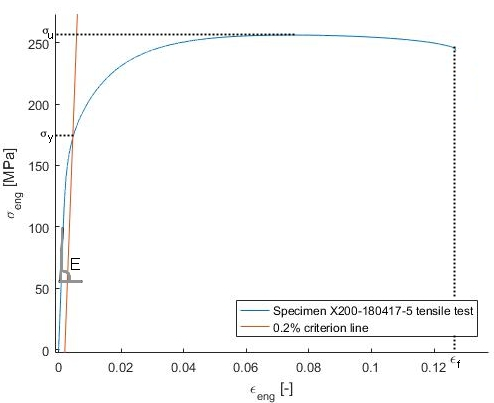
\includegraphics[scale=0.7]{Images/Tract}}
\decoRule
\caption[Tensile stress-strain curve for specimen X200-180417-5 with annotated key features]{Tensile stress-strain curve for specimen X200-180417-5 with annotated key features}
\label{fig:Tract}
\end{figure}


%\subsubsection{Fatigue}


\chapter{Results}
\label{Chap4}
Analyses statistiques etc...
\section{Parameters optimisation}

\section{Reproducibility}
\subsection{Relative density and mechanical properties}

\subsection{Melt pool size and distribution}

\section{Internal properties homogeneity}
As said in section \ref{MMFPP}, all tensile specimens were fabricated vertically. Their height is significantly greater than the other samples'; respectively 6 [cm] and 1 [cm] or less. It was chosen to cut up specimen X200-180417-25 into slices to measure if the density and hardness were homogeneous along the Z direction in the material. The surfaces analysed were named according to their original Z position in the specimen with "B", "C1" , "C2", "C3" and "T" (for bottom, center and top) and to the test done with a letter "D" or "H"  (for density and hardness). The denomination is summarised in figure \ref{fig:saus}.\\

\begin{figure}[th]
\centering
\centerline{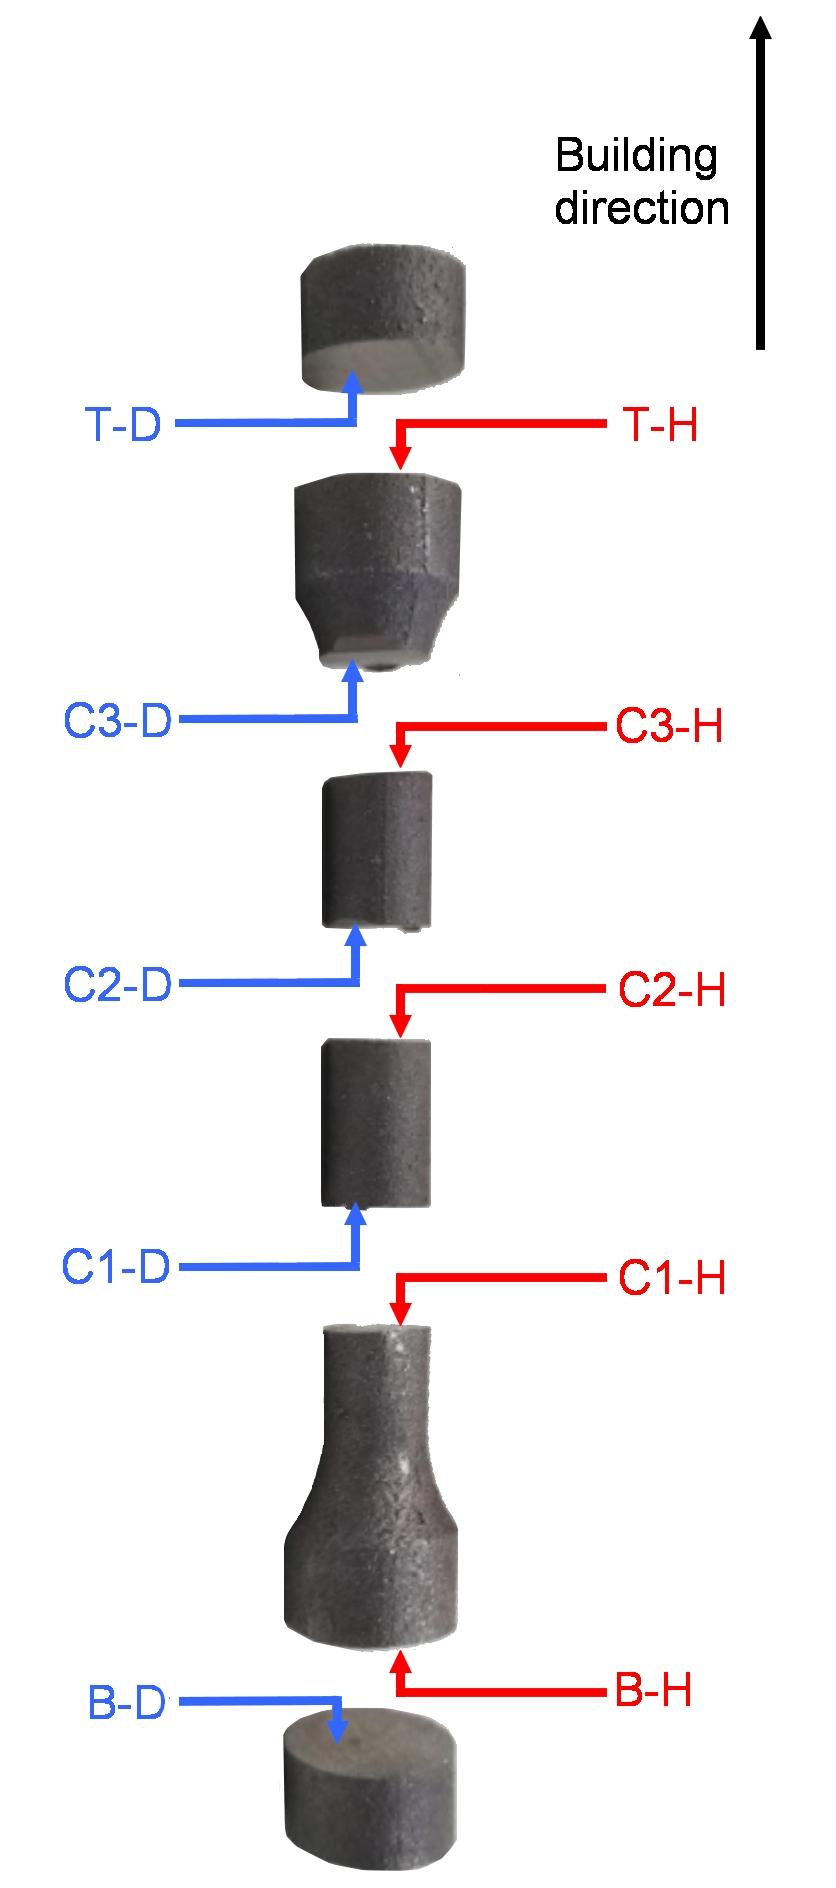
\includegraphics[scale=0.23]{Images/Saus}}
\decoRule
\caption[Specimen X200-180417-25 sub-parts and surfaces denomination]{Specimen X200-180417-25 sub-parts and surfaces denomination.}
\label{fig:saus}
\end{figure}

[Graphe batonnets de H et rho + analyse statistique]

\section{Powder ageing}

\subsection{Grain size and distribution}
\subsubsection{Fresh powder}

\subsubsection{Recycled powder}
\subsection{Composition}

\subsubsection{Fresh powder}

\subsubsection{Recycled powder}
 \begin{center}
\begin{table}[ht]
\begin{tabular}{|c|c |c |c| c|c|}
    \hline
    Date of sampling& Date of last addition of fresh powder & \multicolumn{4}{c}{Composition [\%wt]} \vline\\
    \cline{3-6}
    & & Al& Fe&Mg&Si\\
\hline 
\hline   
    23/10/2017 & 07/09/2017 &89.2&0.12&0.49&10.2\\
    09/01/2018 & 07/09/2017 & 89.3 & 0.13 &0.48&10.1\\
    12/01/2018 & 07/09/2017 & 89.4 & 0.13 &0.48&10\\
    21/02/2018& 07/09/2017 &89.1&0.19&0.51&10.3\\
    13/03/2018& 22/02/2018 &89.1&0.16&0.51&10.1\\    
    \hline
\end{tabular}

\caption[Composition of recycled AlSi10Mg powder as a function of the date]{Composition of recycled AlSi10Mg powder as a function of the date}
\label{tab:compo}
\end{table}
 \end{center}

\section{Heat treatments}

\subsection{Heating process}

\subsection{Microscopy}

\subsection{Hardness testing}

\subsection{Tensile testing}

 \begin{center}
\begin{table}[ht]
\noindent\makebox[\textwidth]{\begin{tabular}{|c|c|c |c |c| c|c|}
    \hline
    Specimen & Contour &  TT & E [GPa] & $\sigma_y$ [MPa] & $\sigma_u$ [MPa] & $\epsilon_f$[\%] \\

\hline
\hline   
    X200-180417-1 & Yes & None & 74.6 & 260.8 & 366.4 & 2.2  \\
    X200-180417-2 & Yes& None & 68.2 & 290.2 & 388.3 & 2.4\\
    X200-180417-3 & Yes& None & 64.0  & 275.9 & - & - \\    
        X200-180417-A& No & None & 61.0 &257.1  & 379.2 & 2.8 \\
    
    X200-180417-7 & Yes& 250$^\circ$C (2h) & 72.2 &230.7 & 334.5 & 9.1 \\
    X200-180417-8 & Yes& 250$^\circ$C (2h) & 70.2 & 238.9 & 347.4 & 8.6 \\
    X200-180417-9 & Yes& 250$^\circ$C (2h) & 71.3 & 227.7 &$\simeq 328.7$ & - \\
    X200-180417-4 & Yes& 300$^\circ$C (2h) & 81.6 & 164.4 & 249.6 & 14.1 \\ 
    X200-180417-5 & Yes& 300$^\circ$C (2h) & 68.4 &172.4 & 256.24 & 13.1 \\
    X200-180417-6 & Yes& 300$^\circ$C (2h) & 68.6 &168.5 & $\simeq 242.5$ & - \\

\hline
\end{tabular}}

\caption[Tensile mechanical properties of the specimens from batch X200-180417]{Tensile mechanical properties of the specimens from batch X200-180417}
\label{tab:pol}
\end{table}
 \end{center}
 
\subsection{Internal stress testing}





%\begin{table}
%\caption{The effects of treatments X and Y on the four groups studied.}
%\label{tab:treatments}
%\centering
%\begin{tabular}{l l l}
%\toprule
%\tabhead{Groups} & \tabhead{Treatment X} & \tabhead{Treatment Y} \\
%\midrule
%1 & 0.2 & 0.8\\
%2 & 0.17 & 0.7\\
%3 & 0.24 & 0.75\\
%4 & 0.68 & 0.3\\
%\bottomrule\\
%\end{tabular}
%\end{table}

\chapter{Discussion}
\label{Chap5}
\section{Powder ageing}
\subsection{Grain size and distribution}

Two trends were identified in section \ref{RGSAD}: there was a clear diminution of the average particle size $D_a$ and a narrowing of the distribution as functions of the number or recycling iterations. Only one sampling did not concur with these observations. This can be easily explained: the powder in question was sampled just after fresh powder was added to the recycled one. Its size distribution was thus shifted back towards a fresher distribution. \\
%modified in a way that is opposed to what recycling causes. \\

Particle sizes going up to $\simeq 134$ [$\mu m$] were measured in the powder samples even though they were sieved with a 75 [$\mu m$] mesh size. The most reasonable justification is that particles agglomeration took place between the siftings and the sizes measurements. Ultrasonic treatments gave the opportunity to confirm that a non-negligible part of the AlSi10Mg powder indeed agglomerated. The maximal measured particle size after exposure to ultrasounds was $\simeq 84$ $[mu m]$. This is rather close to the sieving mesh size but still bigger. The gap between the two could be due to lack of resolution or to residual aggregates.\\

The agglomeration phenomena could explain the diminution of the average particle size with the recycling iterations, according to Maamoud et al. (2018) \cite{Maamoud18}: the large particles that agglomerated since the last sieving could not go through the mesh. Only smaller particles were thus recycled, lowering the average size. Another cause could be the projection of very fine spatters out of the melt pool during the process. These spatters could fall in the unmelted powder and be recycled with the it. Unfortunately, no source could be found literature to support or refute this hypothesis.\\
%. Small particles could also have been preferentially scattered during the SLM process. They would have thus been retrieved in bigger proportion right after

 It seems reasonable to assume that the agglomerates could have led to the emergence of defects in the parts due to powder bed inhomogeneity. This could, at least partly, explain the scatter of relative densities for samples from a same batch. %It may also be a reason behind the remarkably poor properties of sample "8a" (see section \ref{RReprod}).\\
\subsection{Composition}

ICP spectrometry was used in order to estimate the impact of repeated recycling on the evolution of the chemical elements mass fractions. A few observations were made. The prior addition of fresh powder of February sample increased the mass fractions of iron, magnesium, and potentially silicon. It seems that there is a systematic diminution of the alloying elements with the reuse of the powder. Unfortunately, this cannot be attested due to the large error bars.\\

The change of composition induced by SLM was also investigated for two samples. It was concluded that approximately 4\% of the magnesium was lost during the process. The preferential loss of magnesium for a heated aluminium-based alloy is well known \parencite{HIDVEGI197739}. It is due to the lower vapour pressure of the element. %A slight loss of silicon also seemed to have taken place ($\simeq 1\%$) but this cannot be certified.
\section{Density measures assessments}
\label{DDMA}

%\subsection{Hydrostatic weighing}


\subsection{Relative optical density image analysis}
\label{DRODIA}

The estimation of the relative density through RODIA can be imprecise on many aspects. First, the distribution of porosities is inhomogeneous on the analysed surface. Multiple pictures must thus be taken systematically and arbitrarily for each specimen to constitute a representative sample.\\

Second, the quality of the images has a critical role. The isolation of the porosities during the thresholding requires a substantial difference of pixel intensity between the holes and the material. Since some porosities and some zones of the material can appear respectively brighter or darker than was is expected, there are risks that one isolates spots and/or not actual porosities. Additionally, the thresholding is manual and thus prone to slight human errors. \\

Most importantly, the finite resolution of the camera implies that the smallest porosities are not visible on the pictures. One can expect the density measurement through RODIA to be a biased method, due to the discretisation in pixels among other things. Results for pictures with different magnifications were compared to quantify these effects. For this purpose, a picture was taken under 5x magnification and two under 10x magnification. The former was delimited to match the visible zones on the latter (see figure \ref{fig:RODIA1}). The same two zones - named A and B - were thus analysed for different levels of resolution.\\

\begin{figure}[ht]
	\centering
	\centerline{\includegraphics[scale=0.075]{Images/RODIA1}}
	\decoRule
	\caption[5x magnification picture of specimen X200-180319-cub1 and delimitation of the zones A and B]{5x magnification picture of specimen X200-180319-cub1 and delimitation of the zones A and B}
	\label{fig:RODIA1}
\end{figure}

\begin{figure}[ht]
	\centering
	\centerline{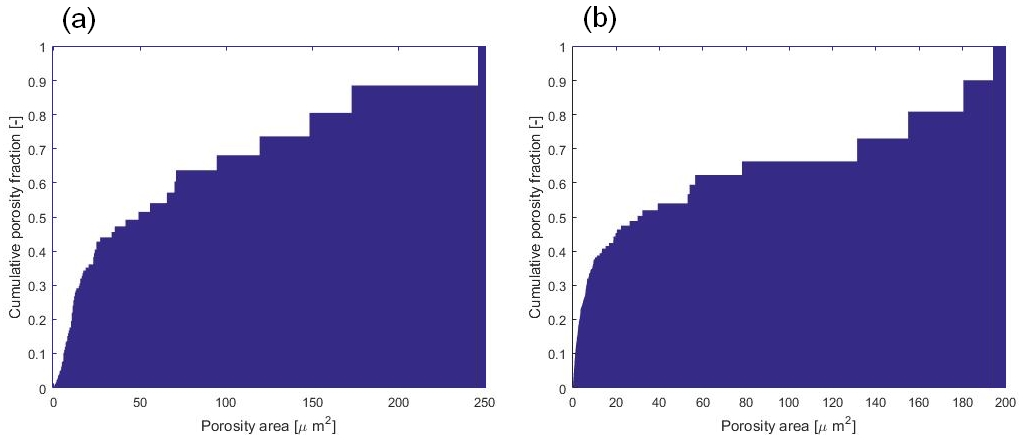
\includegraphics[scale=0.7]{Images/CumSum}}
	\decoRule
	\caption[Cumulative porosity fraction bar chart as function of the porosity area from picture of specimen X200-180319 on zone A under (a) 5x magnification (b) 10x magnification]{Cumulative porosity fraction bar chart as function of the porosity area from picture of specimen X200-180319 on zone A under (a) 5x magnification (b) 10x magnification}
	\label{fig:CumSum}
\end{figure}


The comparison of figures \ref{fig:RODIA2} (b) and (d) shows that much more small porosities are isolated if the resolution is refined. This is confirmed by the bar charts on figure \ref{fig:CumSum}. The threshold of porosity area for detection in the case of 5x magnification is 0.5625 [$\mu m^2$] whereas it is 0.14 [$\mu m^2$] for 10x magnification. This area corresponds to a pixel in each case. It is also worth noting that there is an overall tendency to overestimate the areas at lower resolution, which counterbalances slightly the low number of detected porosities. \\

\begin{figure}[ht]
	\centering
	\centerline{\includegraphics[scale=0.44]{Images/RODIA2}}
	\decoRule
	\caption[Zone A of specimen X200-180319-cub1: (a) Delimitation from original picture under 5x magnification (b) Porosities isolation from 5x magnification picture (c) Original picture under 10x magnification (d) Porosities isolation of 10x magnification picture]{Zone A of specimen X200-180319-cub1: (a) Delimitation from original picture under 5x magnification (b) Porosities isolation from 5x magnification picture (c) Original picture under 10x magnification (d) Porosities isolation of 10x magnification picture}
	\label{fig:RODIA2}
\end{figure}


The RODIA results for zones A and B are outlined in table \ref{tab:RODIASS}. It was observed that pictures with lower resolution have the tendency to lead to the overestimation of the relative density. The order of magnitude of the difference is of few hundredths of percent. The method is thus presumably positively biased. However, the observed effect is minor: this is probably due to the fact that the undetected porosities are the smallest, which influence the less the calculated density value.\\

\begin{center}
	\begin{table}[ht]
		\centerline{\begin{tabular}{|c|c|c|}
				\hline
				Zone & Magnification & Measured relative density [$\%$] \\
				\hline
				A & 5x  & 99.87\\
				A & 10x & 99.84\\
				B & 5x & 99.86\\
				B & 10x & 99.85\\
				\hline
		\end{tabular}}
		\caption[RODIA results for zones A and B of specimen X200-180317 with 5x and 10x magnification]{RODIA results for zones A and B of specimen X200-180317 with 5x and 10x magnification}
		\label{tab:RODIASS}
	\end{table}
\end{center}

Taking pictures at refined magnification could be considered to refine the precision of the method. This would, however, require to increase the number of analysed pictures to generate a sample size as representative. A picture with doubled magnification covers indeed four times less surface. The number of analyses should thus be quadrupled to take as much information into account.\\

RODIA method required to make the assumption that the volumetric porosity fraction is equal the surface one. The dependability of this affirmation will now be discussed. Let us consider a cubic cell of side length D containing a spheric porosity of diameter D in its center (see figure \ref{fig:DDD}). The volumetric porosity fraction $f_v$ is:\\

$$f_v = \frac{\frac{\pi D^3}{6}}{D^3}= \frac{\pi}{6}$$

\begin{figure}[ht]
	\centering
	\centerline{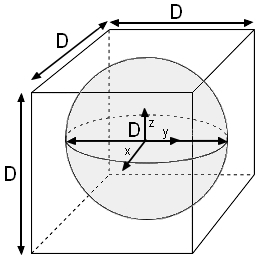
\includegraphics[scale=0.64]{Images/DDD}}
	\decoRule
	\caption[Schematic of a spheric porosity of diameter D in a cubic cell of size length D]{Schematic of a spheric porosity of diameter D in a cubic cell of size length D}
	\label{fig:DDD}
\end{figure}

However, the surface porosity fraction depends on the observed pore diameter $D_{obs}$ which varies with the z coordinate of the surface plane crossing it: $\frac{D_{obs}(z)}{2}=\sqrt{(\frac{D}{2})^2-z^2}$. If we assume that there is a statistically significant number of pores of similar size, one can make the hypothesis that - in average - the observed diameter is the mean diameter $D_{mean}$:\\

$$ \frac{D_{mean}}{2}= \frac{\int_{-\frac{D}{2}}^\frac{D}{2} D_{obs}(z) dz}{D}=\frac{\pi D}{8}$$

This hypothesis is quiet coherent for small pores but not  for the largest: in most cases, a very small number of pores is significantly bigger than the others. If we still assume it to be true, the surface porosity fraction $f_s$ can be computed as follows:

$$f_s=\frac{\frac{\pi D_{mean}^2}{4}}{D^2}=\frac{\pi^3}{16 \cdot 4} \simeq 0.9253 f_v$$

It can thus be concluded that the method to measure the relative density intrinsically has a slightly built-in positive bias. The greater the porosity is, the bigger the bias. In the working range of $\rho_{rel}$ of this work, they can go from 0.01 to 0.03 [\%]. Combining this with the bias induced by the measures imperfections, one can conclude that RODIA should be used as a mean to estimate an upper limit for the relative densities.

\subsection{Measures comparison}
Some samples' densities were also measured through hydrostatic weighing (both with and without preliminary polishing). Multiple techniques were performed on the same few specimens in order to draw a comparison of the results and reach a deeper understanding of the methods reliability. The results are gathered on figures \ref{fig:7comp} and \ref{fig:2comp}.\\

\begin{figure}[ht]
	\centering
	\centerline{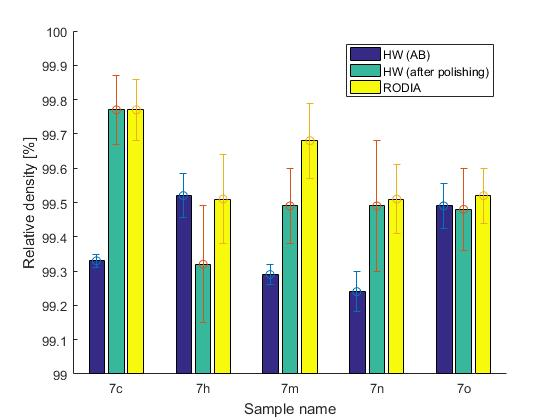
\includegraphics[scale=0.64]{Images/7comp}}
	\decoRule
	\caption[Bar chart of the density measurements with the HW (AB and after polishing) and RODIA methods for samples of batch X200-180109]{Bar charts of the density measurements with the HW (AB and after polishing) and RODIA methods for samples of batch X200-180109}
	\label{fig:7comp}
\end{figure}

\begin{figure}[ht]
	\centering
	\centerline{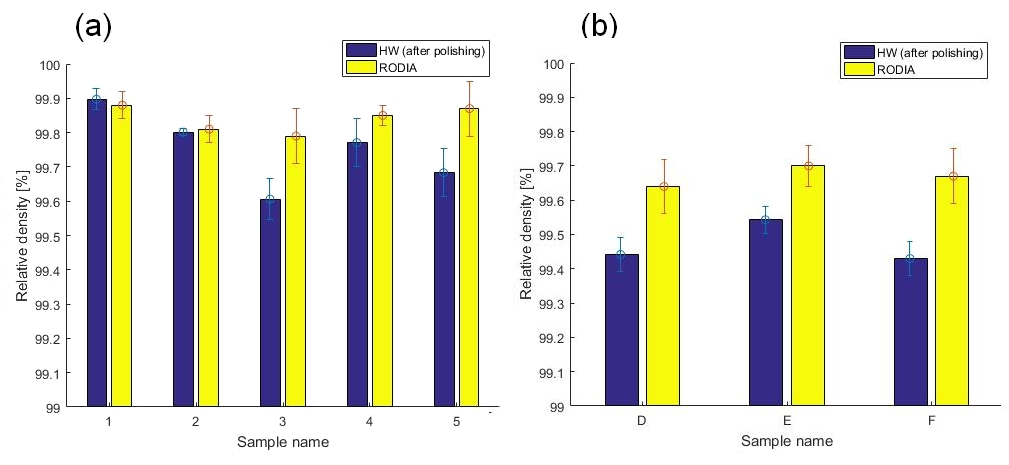
\includegraphics[scale=0.64]{Images/2comp}}
	\decoRule
	\caption[Bar charts of the density measurements with the HW (after polishing) and RODIA methods for samples of (a) batch X200-180319 (b) batch X200-180417]{Bar charts of the density measurements with the HW (after polishing) and RODIA methods for samples of (a) batch X200-180319 (b) batch X200-180417}
	\label{fig:2comp}
\end{figure}

As-built hydro measurements on figure \ref{fig:7comp} demonstrated high variability relatively to the other measures. Over the five tested samples, two exhibited similar relative densities for all techniques. However, three had $\rho_{a,rel}$ significantly below the values obtained with the other methods. In particular, the gap for sample "7c" was 0.44 [\%]. The fact that the CI do not intersect with the others' suggest that AB HW method was negatively biased in those cases. The most plausible explanation is that air was trapped in the surface roughness, which distorted the results (by overestimating the closed porosities volume. This would not be surprising as SLM produced parts usually have bad surface finish.\\ %to observe potential inhomogeneous distributions of the closed porosities in the specimens.

The two other methods were more promising. Relative densities obtained with RODIA method are generally close to the ones of HW after polishing (see figures \ref{fig:7comp} and \ref{fig:2comp}). In average, the absolute difference between the two is 0.16 [\%] (0.24 [\%] at most).  When the difference is greater than 0.02 [\%], the RODIA method always give greater density values. In addition, the CI do not always intersect. This can be attributed to the RODIA positive bias, and potentially to a negative bias for HW - that would still not be fully erased through polishing. Ultimately, given the opposite bias and the proximity of the relative density values for both methods, one could consider the two to be bounds between which lies the actual $\rho_{rel}$.\\

\section{Density and hardness study}

\subsection{Parameters optimisation}
Optimisations of the relative density and hardness were both achieved with the parameters set ($P=0.75 P_{max}=205 [W]$ , $v_s=1200 [\frac{mm}{s}]$). This pair of parameters lie in the process window suggested in section \ref{pp}.
Kempen et al. found optimal parameters values (maximising density) that are not far to the ones of this work (see table \ref{tab:compKemp}) \parencite{Kempen110817}. The energy density was however significantly bigger in this work, especially since the laser was more focused (which is not taken into account for the approximate computation). $E_d$ is rather close to a value minimising porosity obtained by Read et al. (65 $[\frac{J}{mm^3}]$) \parencite{Read150417}. Both cited sources used a chessboard scanning strategy, with islands size of around  5 x 5 [$mm^2$]. \\

\begin{center}
	\begin{table}[ht]
		\centerline{\begin{tabular}{|c|c|c|c|c|c|c|}
				\hline
				Source & h [$\mu m$] & t [$\mu m$]  & $\phi_{99\%} [\mu m]$& P $[W]$ &$v_s [\frac{mm}{sec}]$ & $E_d [\frac{J}{mm^3}]$ \\
				\hline
				This work & 100  & 30 & 75 & 205 & 1200 & 57\\
				\parencite{Kempen110817} & 105 & 30 & 150 & 200 & 1400  & 45 \\
				\parencite{Read150417} & 75 & 30  & 150 & 200 & 1350 & 65 \\				
				\hline
		\end{tabular}}
		\caption[Optimised manufacturing parameters comparison with literature sources]{Optimised manufacturing parameters comparison with literature sources}
		\label{tab:compKemp}
	\end{table}
\end{center}

A relative density of 99.9 [\%] was reached, which is superior to the best values found in the literature \parencite{EOS}. It is likely that all samples manufactured with the optimised parameters had $\rho_{rel}>99.4[\%]$ according to the measurements. Results depended on the powder age and recycling (\ref{RPI}). It can be confirmed that the parameters chosen allowed for a right energy input and a correct melt pools overlapping. \\

The hardness was significantly bigger than what is typically expected - approximately 10 [HV] more (see section \ref{MMABMP}). This could indicate that the microstructure was finer than was is typically obtained or that the material had a more pronounced work hardening ability. At first glance, nothing would justify this. A more credible justification is measurement-related: first, the obtained $H_V$ value depends significantly on the load and on the test's time length. A study showed that the Vickers hardness of aluminium 17-ST alloy - which has a comparable $H_v$ as AlSi10Mg - can range from 130.8 to 143.0 depending on the testing conditions, as shown in table \ref{tab:Vickm} \parencite{Arbtin}. This alone could explain the high hardnesses measured in this work as the load and the time length were both small (respectively 10 [kg] and 10 [sec]).\\

In addition, the indenting machine used necessitates to take manual measurements. Given the high sensitivity of the hardness as a function of the lengths measured, the slightest error is greatly amplified. For example, a length error of 5[$\mu m$], which is the achievable accuracy, induces an error of 4 [HV]. Although the repeated testing greatly improves the estimation reliability (see confidence intervals in section \ref{Rparaopti}), a slight negative bias could induce a systematic overestimation of the hardness by a few [HV]. For these reasons, the hardness values obtained in this work should not be compared to the ones in literature. However, they still can be compared to each other as they were obtained through the same procedure.\\

\begin{table}[ht]
		\centering
			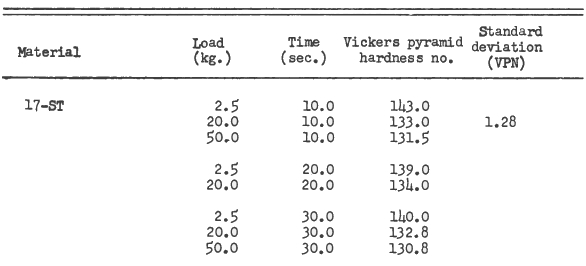
\includegraphics[scale=0.90]{Images/Vickm}
			\decoRule
		\caption[Vickers hardness results data for aluminium 17-ST alloy.]{Vickers hardness results data for aluminium 17-ST alloy (from Emil Arbtin Jr. and Glenn Murphy, 1953 \parencite{Arbtin}).}
		\label{tab:Vickm}
\end{table}

Furthermore, one should note that the optimisation of the overall density was perhaps not the most pertinent to conduct. As it will be discussed in section \ref{DMPP}, it is very likely that the tensile mechanical properties are dictated by the residual stresses and by the effects due to a second population of porosities. It could thus be interesting to perform a parametric study putting these at the forefront.\\ 

\subsection{Reproducibility}

SLM process demonstrated a satisfying reproducibility for the optimised set of parameters. However, non optimal values (P=0.75$P_{max}$,$v_s=900 [\frac{mm}{sec}]$) lead to higher variability for the hardness and the relative density. Since the energy density is bigger in that case ($76[\frac{J}{mm^3}]$), the explanation could be that the heat input was sufficient to trigger key hole instability at times, inducing porosity inside the melt pools. The phenomenon is illustrated in figure \ref{fig:KHI}. \\

\begin{figure}[ht]
	\centering
	\centerline{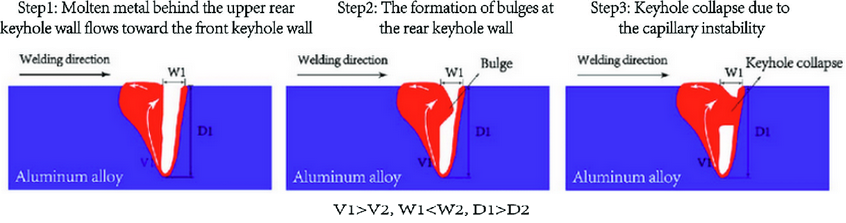
\includegraphics[scale=0.52]{Images/KHI}}
	\decoRule
	\caption[The diagram of keyhole collapse caused by the keyhole instability.]{The diagram of keyhole collapse caused by the keyhole instability (from Huang et al., 2017 \parencite{Huang2017})}
	\label{fig:KHI}
\end{figure}

Relative density tended to be bigger for the samples of parameters (P=0.75$P_{max}$,$v_s=900 [\frac{mm}{sec}]$) scanned tardily. It may be due to the longer time left to exchange heat with the nearby unsintered powder. If the first scanned samples stayed at a significantly higher temperature compared to the others, they could be more prone to exceed the threshold leading to key hole instability. They would also have a bigger hydrogen solubility, as it increases with temperature (see figure \ref{fig:Solub}) \parencite{Verhaeghe}. The apparition of porosities would thus be facilitated. \\

One sample, named X200-171024-8a, had notably low relative density. Its melt pools size distribution was compared to another specimen's (see section \ref{rs_mps}): the former was more homogeneous. Lots of porosities were present at the pools interface, which confirms that poor overlapping was achieved. The origin of this problem was not sorted out. \\


\begin{figure}[ht]
	\centering
	\centerline{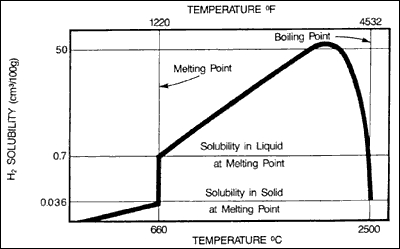
\includegraphics[scale=0.75]{Images/Solub}}
	\decoRule
	\caption[Solubility of hydrogen in aluminium.]{Solubility of hydrogen in aluminium (from Verhaeghe et al., 2003 \parencite{Verhaeghe})}
	\label{fig:Solub}
\end{figure}

The hypothesis of thermal influence do not seem to stand for the specimens made with the optimised parameters. The energy density is 33\% inferior, so the temperature must have reached lower values. No trend could thus be observed. The most determinant variables in terms of density and hardness seem to be the composition and the grain size distribution of the powder. A superior relative density was obtained after fresh powder was added to the recycled one (see section \ref{RPI}). However, an additional recycling iteration of the same powder caused a sensible decrease of $\rho_{rel}$. It dovetailed with a diminution of the alloying elements mass fractions. It is possible that both trends were correlated. Another possibility is that the contamination with moisture exceeded a critical value. The latter cannot be measured with ICP so this could not be verified.

\section{Mechanical properties}
\label{DMPP}
The average tensile properties measures for AB specimens fell a bit short of the expectations. While $\sigma_y$ was elavated compared to the standards, $\sigma_u$ was less satisfactory ($\simeq 17\%$ beneath the highest value \parencite{EOS}). In addition, $\epsilon_f$ was lower than most values in table \ref{tab:Kemp1}: up to $\simeq 58\%$ less than other results for samples built along z. \\%Furthermore, while $E$ varies a lot in literature, it is extremely rare that it reaches an average value as low as 65. \\

Results were compared to the \textit{Aerostream} project's carried out by ULB, VUB and UCL universities in which AlSi10Mg tensile specimens were also built vertically and tested. The process parameters used for the project are unfortunately undisclosed. The comparison of the AB specimens is presented on figure \ref{fig:AerAB}. The properties obtained with the \textit{Aerostream} project are obviously far better than what was obtained in this thesis for as-built specimens (and to what can be found in literature). The fracture strain was indeed three times bigger and the ultimate tensile strength 24\% superior. \\

\begin{figure}[ht]
	\centering
	\centerline{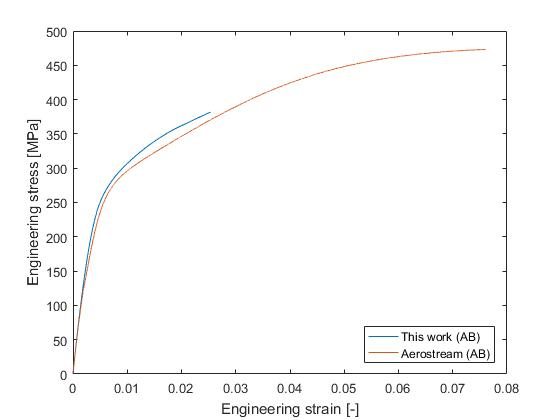
\includegraphics[scale=0.64]{Images/AerAB}}
	\decoRule
	\caption[Engineering stress-strain tensile curves for as-built specimens of this work (in average) and of \textit{Aerostream} project]{Engineering stress-strain tensile curves for as-built specimens of this work (in average) and of \textit{Aerostream} project}
	\label{fig:AerAB}
\end{figure}

The shortcomings of the manufactured samples can be attributed at least partially to the presence of residual stresses. Consequent tension residual stresses were measured in the material. The actual stress during the tensile tests was thus greater than what was measured. In addition, there is a stress concentration due to the porosities. For spherical porosities, it is given by:

$$\sigma_{loc}=K_t \cdot \sigma_{t} $$

where $\sigma_t$ is the applied stress and $K_t=\frac{3}{2}(1+\frac{2}{7-5\nu}) \simeq 2$ [-] is the stress intensity factor \parencite{Paris}. \\

The combination of the effects must have caused a shift of the actual local stress. The critical stress  $\sigma_c$ causing crack propagation was thus attained before the start of the voids coalescence, as illustrated in figure \ref{fig:RSTrac}. As a result, the apparent tensile curve was truncated, reducing slightly $\sigma_u$ and greatly $\epsilon_f$. The yield strength, however, was the same as a residual stress free sample. \\

\begin{figure}[ht]
	\centering
	\centerline{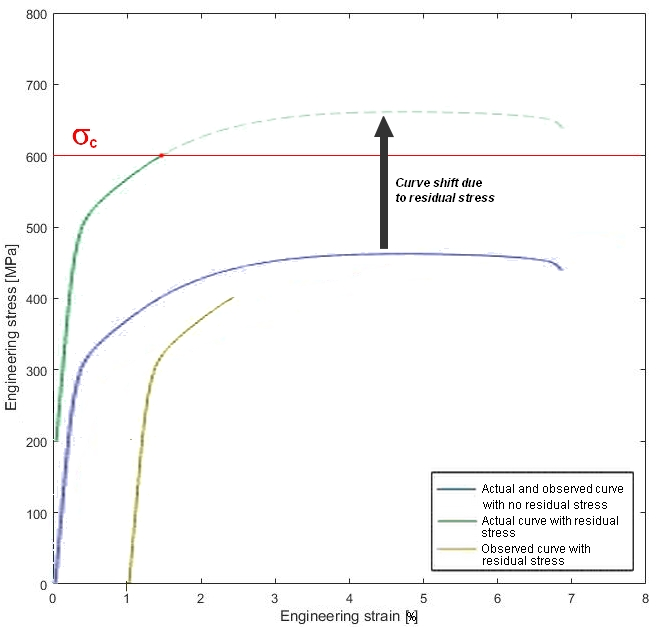
\includegraphics[scale=0.53]{Images/RSTrac}}
	\decoRule
	\caption[Illustration of the impact of residual stress on the observed tensile stress-strain curve]{Illustration of the impact of residual stress on the observed tensile stress-strain curve}
	\label{fig:RSTrac}
\end{figure}

This concurs with the data of table \ref{tab:Wang}: the heating of the plate during the manufacturing process at 160$^\circ C$, while reducing the residual stresses, increased the fracture strain by 77\%. This could explain the differences with the better properties found in literature: as all the sources that obtained both high $\sigma_u$ and $\epsilon_f$ did not specify the used process conditions, it is conceivable that they all used plate heating. \\

A consequent increase of ductility was observed for samples heat treated at 250$\sigma$ and higher temperatures. This is due to the softening of the material induced by the microstructure modifications (see section \ref{DMMM}). It could also be due to stress relief (SR). However, SR is not necessary to explain the results: the lowered maximal stress due to the softening could simply have been insufficient to reach the critical value $\sigma_c$ impeding the ductile damage mechanism. The curves can thus not enable to certify if there was stress relief or not. Nevertheless, the heat treatment at 250$^\circ C$ permitted to have a good trade-off for the tensile properties: there was an increase of 250\% of $\epsilon_f$ for decreases of only 12\% and 11\% of $\sigma_y$ and $\sigma_u$ respectively. This is quiet different from what Mertens et al. observed for the same treatment (80\% increase for $\epsilon_f$ and decreases of 10\% and 2\% for $\sigma_y$ and $\sigma_u$) \parencite{Mertens15}.\\

An increase of ultimate tensile strength was observed for the specimens that underwent a heat treatment at 150$^\circ$C. This is seemingly due to artificial ageing: precipitated $Mg_2Si$ particles constrain the dislocations displacement through the Orowan bowing phenomena as shown in figure \ref{fig:Oro}, which induces hardening \parencite{Ghosh}. Artificial ageing can take place at 160$^\circ$C (see section \ref{SOTAPT}), it thus do not seem far-fetched that it could happen ten degrees below. Sample heated at 200$^\circ C$ demonstrated properties similar to the as-built ones. This is probably due to the compensation of the age-hardening effect with the microstructure softening.\\

\begin{figure}[ht]
	\centering
	\centerline{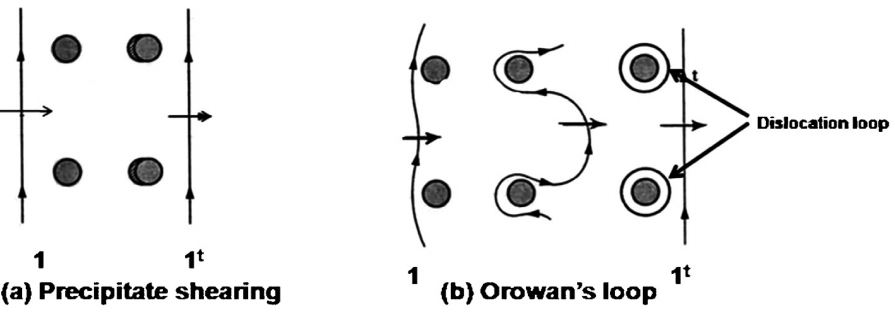
\includegraphics[scale=0.45]{Images/Orowan}}
	\decoRule
	\caption[Schematic representation of dislocation/precipitate interaction under different tempering condition (a) underaged, (b) peak aged]{Schematic representation of dislocation/precipitate interaction under different tempering condition (a) underaged, (b) peak aged (from Ghosh et al., 2015 \parencite{Ghosh})}
	\label{fig:Oro}
\end{figure}

A noteworthy parallel can be made between the Vickers hardness and the ultimate tensile strength for AB and heat treated samples. The two are connected via a quasi-linear relationship as shown in table \ref{tab:HVUTS} and figure \ref{fig:HVUTS}. A good empirical approximation can thus be obtained with $\sigma_u \simeq 2.88 H_v$. Data was taken from sections \ref{RCABS} and \ref{RCHTS}.

\begin{center}
	\begin{table}[ht]
		\centerline{\begin{tabular}{|c|c|c|c|}
				\hline
				HT & $H_v$ [HV] & $\sigma_u$ [MPa] & $\frac{H_v}{\sigma_u}$ $[\frac{HV}{MPa}]$ \\
				\hline
				AB & 136  & 381.7&2.81\\
				150$^\circ$ &151.0 & 441.7 & 2.93\\
				200$^\circ$  &133.6& 382.0 & 2.86\\
				250$^\circ$  &118.6&340.9 & 2.87\\
				300$^\circ$  &86.7& 252.9 & 2.92\\
				\hline
		\end{tabular}}
		\caption[Relationship between Vickers hardness and ultimate tensile strength]{Relationship between Vickers hardness and ultimate tensile strength}
		\label{tab:HVUTS}
	\end{table}
\end{center}

\begin{figure}[ht]
	\centering
	\centerline{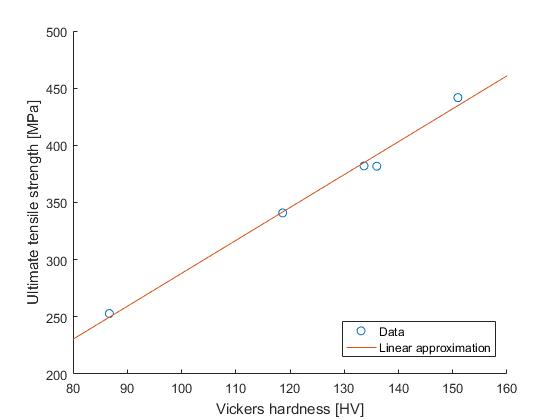
\includegraphics[scale=0.64]{Images/HVUTS}}
	\decoRule
	\caption[Average ultimate tensile strength for each heat treatment as a function of the Vickers hardness]{Average ultimate tensile strength for each heat treatment as a function of the Vickers hardness}
	\label{fig:HVUTS}
\end{figure}

\section{Microstructure}
\label{DMMM}

%Step-like structures of width length similar to the hatch space were observed. It would suggest that failure takes place at the boundary between melt pools, where the microstructure is coarser, as discussed by Aboulkhair et al. \cite{Rosenthal17}.\\
%[Mécanisme d'endommagement: deux populations de porosités? A confirmer/ infirmer avec les articles envoyés par AS]
[Taille des cupules= ordre de grandeur des éléments de la microstructure?] 

[Modèle pour la sphéroisisation: rien dans la literature pour notre microstructure (? j'ai rien trouvé en faisant une petite recherche)]
[Trajet de fissure "accidenté"? Déviation par les défauts?]

The use of the nearest neighbour distance for the globularized samples as a comparison with cell size is probably not the most pertinent choice. Indeed, 

\section{Heating process}
Quand on chauffe à 300 deg, on chauffe déjà longtemps à plus de 200 deg.

 On garde cette partie ou pas?
 
 Je pense que oui, mais elle ne va pas être très longue.

%Residual stress à discuter dans mechanical properties ok?
%\section{Residual stresses}

%[XRD: pièce as-built a un plus petit spread que ceux avec TT à basse T, p-e parce que cube coupé en 2 => relaxation des contraintes après fab?]

%While the usual stress-relief treatment for aluminium alloys -to hours holding at 300$^\circ$ C- does indeed relieve stresses inside the specimen, it also triggers significantly the diffusion of alloying elements, altering the material microstructure.



\label{D-MP}

\section{Residual stresses}
Residual stresses measured with the hole method for an as-built sample were inferior to the ones of a specimen treated at 300$^\circ C$. Other samples were sent for analysis, but the results were not received when this work was submitted due to logistical issues: the specimens were analysed in Malta, causing considerable transport time.\\

%X-ray diffraction method measurements suggested that the as-built sample had a similar amount of residual or less residual stresses compared to the heat treated samples. For heat treated samples, a diminution of residual stresses was measured as a a function of temperature. However, this trend could be insignificant as the measurements were far from was obtained in literature for stress-free samples. 

According to Vashista et al. (2012) \cite{Vashista12}, direct mathematical relation between FWHM and residual stresses is difficult to obtain, because FWHM is known to increase with plastic deformation and grain refinement besides residual stress. They however observed experimentally a non-linear increase of FWHM with residual stresses.\\

We indeed observe a decrease of FWHM with the temperature of the heat treatment. It would mean that the heat treatment relieves stresses as intended. Only the as-built sample seems to defy this logic and present a FWHM lower than some heat-treated samples. However this could be explained by the geometrical difference of the as-built. While the heat-treated samples used for XRD are complete 5 x 5 x 5 [mm$^3$] cubes, the as-built is 1 x 1 x 1 [cm$^3$] cube cut in half. The higher volume explains the higher peak, and the cut may have allow a part of the residual stresses to relax by deforming the part, and thus causing the narrowing of the peak.\\

Nonetheless, the sample heat-treated at 300$^\circ$C for 2 hours remains far from stress-free according to the results from Lam et al. (2015) \cite{Lam15}. They obtained for the same peak a FWHM of 0.361, which much smaller than everything we managed to obtain. However, as discussed above, other parameters could play a role in this difference.

\section{Optimisation}



%\section{Mechanical testing}


\chapter{Conclusion}
\label{Chap6}
%\textcolor{gray}{They incorporate in a synthetic way the main results and compare them with the
%initial objectives. Generally, this final chapter also presents prospects for the continuation of the
%work undertaken.}
In this master thesis, an analysis of the impact of stress relief heat treatments was carried out. Results for the residual stresses measurements were unsatisfactory: they suggested that the residual stresses of heat treated samples were equivalent to or bigger than the ones of as-built samples. A possible explanation was provided.\\

Nevertheless, multiple instructive observations were made. The importance of powder monitoring was first highlighted. The assessment of the relative density measurements was then conducted. Results indicated that hydrostatic weighing (after polishing) and relative optical density image analysis methods could constitute bound values for the actual relative density value.\\

Optimal process parameters were identified with the aim of achieving high relative density. The reproducibility was addressed, both for the optimal parameters and for suboptimal ones. The former led to relative density values ranging from 99.4\% to 99.9\%. High hardness values were obtained compared to literature. The underlying reasons were identified.\\

Plausible hypotheses were made to explain the mechanical properties for as-built and heat-treated specimens. The major role of residual stresses was emphasised. The use of a pre-heating plate during the manufacturing process seems to substantially improve the tensile properties. An empirical relationship linking the ultimate tensile strength to the hardness was suggested.\\

The direct link between the very fine microstructure of SLM parts and their mechanical properties was discussed. Heat treatments have shown to affect deeply the microstructure, mainly by the process of spheroidization. Design of heat treatments specifically thought for AM alloys is necessary to ensure better control of the final properties.

This thesis leaves open numerous paths of investigation. An in-depth analysis of the variables influencing the residual stresses - such as machining and heat treatment conditions - could bring clarity regarding the reasons behind the surprising results of this work. A manufacturing process optimisation could also be carried out to minimise the residuals stresses in the parts, as their critical role was pointed out. Finally, other inherent issues of SLM should be addressed, such as fatigue strength.\\
%Consequently, although the principal goal of the thesis was not achieved, some 


%
%% Chapter 1

\chapter{Chapter Title Here} % Main chapter title

\label{Chapter1} % For referencing the chapter elsewhere, use \ref{Chapter1} 

%----------------------------------------------------------------------------------------

% Define some commands to keep the formatting separated from the content 
\newcommand{\keyword}[1]{\textbf{#1}}
\newcommand{\tabhead}[1]{\textbf{#1}}
\newcommand{\code}[1]{\texttt{#1}}
\newcommand{\file}[1]{\texttt{\bfseries#1}}
\newcommand{\option}[1]{\texttt{\itshape#1}}

%----------------------------------------------------------------------------------------

\section{Welcome and Thank You}
Welcome to this \LaTeX{} Thesis Template, a beautiful and easy to use template for writing a thesis using the \LaTeX{} typesetting system.

If you are writing a thesis (or will be in the future) and its subject is technical or mathematical (though it doesn't have to be), then creating it in \LaTeX{} is highly recommended as a way to make sure you can just get down to the essential writing without having to worry over formatting or wasting time arguing with your word processor.

\LaTeX{} is easily able to professionally typeset documents that run to hundreds or thousands of pages long. With simple mark-up commands, it automatically sets out the table of contents, margins, page headers and footers and keeps the formatting consistent and beautiful. One of its main strengths is the way it can easily typeset mathematics, even \emph{heavy} mathematics. Even if those equations are the most horribly twisted and most difficult mathematical problems that can only be solved on a super-computer, you can at least count on \LaTeX{} to make them look stunning.

%----------------------------------------------------------------------------------------

\section{Learning \LaTeX{}}

\LaTeX{} is not a \textsc{wysiwyg} (What You See is What You Get) program, unlike word processors such as Microsoft Word or Apple's Pages. Instead, a document written for \LaTeX{} is actually a simple, plain text file that contains \emph{no formatting}. You tell \LaTeX{} how you want the formatting in the finished document by writing in simple commands amongst the text, for example, if I want to use \emph{italic text for emphasis}, I write the \verb|\emph{text}| command and put the text I want in italics in between the curly braces. This means that \LaTeX{} is a \enquote{mark-up} language, very much like HTML.

\subsection{A (not so short) Introduction to \LaTeX{}}

If you are new to \LaTeX{}, there is a very good eBook -- freely available online as a PDF file -- called, \enquote{The Not So Short Introduction to \LaTeX{}}. The book's title is typically shortened to just \emph{lshort}. You can download the latest version (as it is occasionally updated) from here:
\url{http://www.ctan.org/tex-archive/info/lshort/english/lshort.pdf}

It is also available in several other languages. Find yours from the list on this page: \url{http://www.ctan.org/tex-archive/info/lshort/}

It is recommended to take a little time out to learn how to use \LaTeX{} by creating several, small `test' documents, or having a close look at several templates on:\\ 
\url{http://www.LaTeXTemplates.com}\\ 
Making the effort now means you're not stuck learning the system when what you \emph{really} need to be doing is writing your thesis.

\subsection{A Short Math Guide for \LaTeX{}}

If you are writing a technical or mathematical thesis, then you may want to read the document by the AMS (American Mathematical Society) called, \enquote{A Short Math Guide for \LaTeX{}}. It can be found online here:
\url{http://www.ams.org/tex/amslatex.html}
under the \enquote{Additional Documentation} section towards the bottom of the page.

\subsection{Common \LaTeX{} Math Symbols}
There are a multitude of mathematical symbols available for \LaTeX{} and it would take a great effort to learn the commands for them all. The most common ones you are likely to use are shown on this page:
\url{http://www.sunilpatel.co.uk/latex-type/latex-math-symbols/}

You can use this page as a reference or crib sheet, the symbols are rendered as large, high quality images so you can quickly find the \LaTeX{} command for the symbol you need.

\subsection{\LaTeX{} on a Mac}
 
The \LaTeX{} distribution is available for many systems including Windows, Linux and Mac OS X. The package for OS X is called MacTeX and it contains all the applications you need -- bundled together and pre-customized -- for a fully working \LaTeX{} environment and work flow.
 
MacTeX includes a custom dedicated \LaTeX{} editor called TeXShop for writing your `\file{.tex}' files and BibDesk: a program to manage your references and create your bibliography section just as easily as managing songs and creating playlists in iTunes.

%----------------------------------------------------------------------------------------

\section{Getting Started with this Template}

If you are familiar with \LaTeX{}, then you should explore the directory structure of the template and then proceed to place your own information into the \emph{THESIS INFORMATION} block of the \file{main.tex} file. You can then modify the rest of this file to your unique specifications based on your degree/university. Section \ref{FillingFile} on page \pageref{FillingFile} will help you do this. Make sure you also read section \ref{ThesisConventions} about thesis conventions to get the most out of this template.

If you are new to \LaTeX{} it is recommended that you carry on reading through the rest of the information in this document.

Before you begin using this template you should ensure that its style complies with the thesis style guidelines imposed by your institution. In most cases this template style and layout will be suitable. If it is not, it may only require a small change to bring the template in line with your institution's recommendations. These modifications will need to be done on the \file{MastersDoctoralThesis.cls} file.

\subsection{About this Template}

This \LaTeX{} Thesis Template is originally based and created around a \LaTeX{} style file created by Steve R.\ Gunn from the University of Southampton (UK), department of Electronics and Computer Science. You can find his original thesis style file at his site, here:
\url{http://www.ecs.soton.ac.uk/~srg/softwaretools/document/templates/}

Steve's \file{ecsthesis.cls} was then taken by Sunil Patel who modified it by creating a skeleton framework and folder structure to place the thesis files in. The resulting template can be found on Sunil's site here:
\url{http://www.sunilpatel.co.uk/thesis-template}

Sunil's template was made available through \url{http://www.LaTeXTemplates.com} where it was modified many times based on user requests and questions. Version 2.0 and onwards of this template represents a major modification to Sunil's template and is, in fact, hardly recognisable. The work to make version 2.0 possible was carried out by \href{mailto:vel@latextemplates.com}{Vel} and Johannes Böttcher.

%----------------------------------------------------------------------------------------

\section{What this Template Includes}

\subsection{Folders}

This template comes as a single zip file that expands out to several files and folders. The folder names are mostly self-explanatory:

\keyword{Appendices} -- this is the folder where you put the appendices. Each appendix should go into its own separate \file{.tex} file. An example and template are included in the directory.

\keyword{Chapters} -- this is the folder where you put the thesis chapters. A thesis usually has about six chapters, though there is no hard rule on this. Each chapter should go in its own separate \file{.tex} file and they can be split as:
\begin{itemize}
\item Chapter 1: Introduction to the thesis topic
\item Chapter 2: Background information and theory
\item Chapter 3: (Laboratory) experimental setup
\item Chapter 4: Details of experiment 1
\item Chapter 5: Details of experiment 2
\item Chapter 6: Discussion of the experimental results
\item Chapter 7: Conclusion and future directions
\end{itemize}
This chapter layout is specialised for the experimental sciences, your discipline may be different.

\keyword{Figures} -- this folder contains all figures for the thesis. These are the final images that will go into the thesis document.

\subsection{Files}

Included are also several files, most of them are plain text and you can see their contents in a text editor. After initial compilation, you will see that more auxiliary files are created by \LaTeX{} or BibTeX and which you don't need to delete or worry about:

\keyword{example.bib} -- this is an important file that contains all the bibliographic information and references that you will be citing in the thesis for use with BibTeX. You can write it manually, but there are reference manager programs available that will create and manage it for you. Bibliographies in \LaTeX{} are a large subject and you may need to read about BibTeX before starting with this. Many modern reference managers will allow you to export your references in BibTeX format which greatly eases the amount of work you have to do.

\keyword{MastersDoctoralThesis.cls} -- this is an important file. It is the class file that tells \LaTeX{} how to format the thesis. 

\keyword{main.pdf} -- this is your beautifully typeset thesis (in the PDF file format) created by \LaTeX{}. It is supplied in the PDF with the template and after you compile the template you should get an identical version.

\keyword{main.tex} -- this is an important file. This is the file that you tell \LaTeX{} to compile to produce your thesis as a PDF file. It contains the framework and constructs that tell \LaTeX{} how to layout the thesis. It is heavily commented so you can read exactly what each line of code does and why it is there. After you put your own information into the \emph{THESIS INFORMATION} block -- you have now started your thesis!

Files that are \emph{not} included, but are created by \LaTeX{} as auxiliary files include:

\keyword{main.aux} -- this is an auxiliary file generated by \LaTeX{}, if it is deleted \LaTeX{} simply regenerates it when you run the main \file{.tex} file.

\keyword{main.bbl} -- this is an auxiliary file generated by BibTeX, if it is deleted, BibTeX simply regenerates it when you run the \file{main.aux} file. Whereas the \file{.bib} file contains all the references you have, this \file{.bbl} file contains the references you have actually cited in the thesis and is used to build the bibliography section of the thesis.

\keyword{main.blg} -- this is an auxiliary file generated by BibTeX, if it is deleted BibTeX simply regenerates it when you run the main \file{.aux} file.

\keyword{main.lof} -- this is an auxiliary file generated by \LaTeX{}, if it is deleted \LaTeX{} simply regenerates it when you run the main \file{.tex} file. It tells \LaTeX{} how to build the \emph{List of Figures} section.

\keyword{main.log} -- this is an auxiliary file generated by \LaTeX{}, if it is deleted \LaTeX{} simply regenerates it when you run the main \file{.tex} file. It contains messages from \LaTeX{}, if you receive errors and warnings from \LaTeX{}, they will be in this \file{.log} file.

\keyword{main.lot} -- this is an auxiliary file generated by \LaTeX{}, if it is deleted \LaTeX{} simply regenerates it when you run the main \file{.tex} file. It tells \LaTeX{} how to build the \emph{List of Tables} section.

\keyword{main.out} -- this is an auxiliary file generated by \LaTeX{}, if it is deleted \LaTeX{} simply regenerates it when you run the main \file{.tex} file.

So from this long list, only the files with the \file{.bib}, \file{.cls} and \file{.tex} extensions are the most important ones. The other auxiliary files can be ignored or deleted as \LaTeX{} and BibTeX will regenerate them.

%----------------------------------------------------------------------------------------

\section{Filling in Your Information in the \file{main.tex} File}\label{FillingFile}

You will need to personalise the thesis template and make it your own by filling in your own information. This is done by editing the \file{main.tex} file in a text editor or your favourite LaTeX environment.

Open the file and scroll down to the third large block titled \emph{THESIS INFORMATION} where you can see the entries for \emph{University Name}, \emph{Department Name}, etc \ldots

Fill out the information about yourself, your group and institution. You can also insert web links, if you do, make sure you use the full URL, including the \code{http://} for this. If you don't want these to be linked, simply remove the \verb|\href{url}{name}| and only leave the name.

When you have done this, save the file and recompile \code{main.tex}. All the information you filled in should now be in the PDF, complete with web links. You can now begin your thesis proper!

%----------------------------------------------------------------------------------------

\section{The \code{main.tex} File Explained}

The \file{main.tex} file contains the structure of the thesis. There are plenty of written comments that explain what pages, sections and formatting the \LaTeX{} code is creating. Each major document element is divided into commented blocks with titles in all capitals to make it obvious what the following bit of code is doing. Initially there seems to be a lot of \LaTeX{} code, but this is all formatting, and it has all been taken care of so you don't have to do it.

Begin by checking that your information on the title page is correct. For the thesis declaration, your institution may insist on something different than the text given. If this is the case, just replace what you see with what is required in the \emph{DECLARATION PAGE} block.

Then comes a page which contains a funny quote. You can put your own, or quote your favourite scientist, author, person, and so on. Make sure to put the name of the person who you took the quote from.

Following this is the abstract page which summarises your work in a condensed way and can almost be used as a standalone document to describe what you have done. The text you write will cause the heading to move up so don't worry about running out of space.

Next come the acknowledgements. On this page, write about all the people who you wish to thank (not forgetting parents, partners and your advisor/supervisor).

The contents pages, list of figures and tables are all taken care of for you and do not need to be manually created or edited. The next set of pages are more likely to be optional and can be deleted since they are for a more technical thesis: insert a list of abbreviations you have used in the thesis, then a list of the physical constants and numbers you refer to and finally, a list of mathematical symbols used in any formulae. Making the effort to fill these tables means the reader has a one-stop place to refer to instead of searching the internet and references to try and find out what you meant by certain abbreviations or symbols.

The list of symbols is split into the Roman and Greek alphabets. Whereas the abbreviations and symbols ought to be listed in alphabetical order (and this is \emph{not} done automatically for you) the list of physical constants should be grouped into similar themes.

The next page contains a one line dedication. Who will you dedicate your thesis to?

Finally, there is the block where the chapters are included. Uncomment the lines (delete the \code{\%} character) as you write the chapters. Each chapter should be written in its own file and put into the \emph{Chapters} folder and named \file{Chapter1}, \file{Chapter2}, etc\ldots Similarly for the appendices, uncomment the lines as you need them. Each appendix should go into its own file and placed in the \emph{Appendices} folder.

After the preamble, chapters and appendices finally comes the bibliography. The bibliography style (called \option{authoryear}) is used for the bibliography and is a fully featured style that will even include links to where the referenced paper can be found online. Do not underestimate how grateful your reader will be to find that a reference to a paper is just a click away. Of course, this relies on you putting the URL information into the BibTeX file in the first place.

%----------------------------------------------------------------------------------------

\section{Thesis Features and Conventions}\label{ThesisConventions}

To get the best out of this template, there are a few conventions that you may want to follow.

One of the most important (and most difficult) things to keep track of in such a long document as a thesis is consistency. Using certain conventions and ways of doing things (such as using a Todo list) makes the job easier. Of course, all of these are optional and you can adopt your own method.

\subsection{Printing Format}

This thesis template is designed for double sided printing (i.e. content on the front and back of pages) as most theses are printed and bound this way. Switching to one sided printing is as simple as uncommenting the \option{oneside} option of the \code{documentclass} command at the top of the \file{main.tex} file. You may then wish to adjust the margins to suit specifications from your institution.

The headers for the pages contain the page number on the outer side (so it is easy to flick through to the page you want) and the chapter name on the inner side.

The text is set to 11 point by default with single line spacing, again, you can tune the text size and spacing should you want or need to using the options at the very start of \file{main.tex}. The spacing can be changed similarly by replacing the \option{singlespacing} with \option{onehalfspacing} or \option{doublespacing}.

\subsection{Using US Letter Paper}

The paper size used in the template is A4, which is the standard size in Europe. If you are using this thesis template elsewhere and particularly in the United States, then you may have to change the A4 paper size to the US Letter size. This can be done in the margins settings section in \file{main.tex}.

Due to the differences in the paper size, the resulting margins may be different to what you like or require (as it is common for institutions to dictate certain margin sizes). If this is the case, then the margin sizes can be tweaked by modifying the values in the same block as where you set the paper size. Now your document should be set up for US Letter paper size with suitable margins.

\subsection{References}

The \code{biblatex} package is used to format the bibliography and inserts references such as this one \parencite{Reference1}. The options used in the \file{main.tex} file mean that the in-text citations of references are formatted with the author(s) listed with the date of the publication. Multiple references are separated by semicolons (e.g. \parencite{Reference2, Reference1}) and references with more than three authors only show the first author with \emph{et al.} indicating there are more authors (e.g. \parencite{Reference3}). This is done automatically for you. To see how you use references, have a look at the \file{Chapter1.tex} source file. Many reference managers allow you to simply drag the reference into the document as you type.

Scientific references should come \emph{before} the punctuation mark if there is one (such as a comma or period). The same goes for footnotes\footnote{Such as this footnote, here down at the bottom of the page.}. You can change this but the most important thing is to keep the convention consistent throughout the thesis. Footnotes themselves should be full, descriptive sentences (beginning with a capital letter and ending with a full stop). The APA6 states: \enquote{Footnote numbers should be superscripted, [...], following any punctuation mark except a dash.} The Chicago manual of style states: \enquote{A note number should be placed at the end of a sentence or clause. The number follows any punctuation mark except the dash, which it precedes. It follows a closing parenthesis.}

The bibliography is typeset with references listed in alphabetical order by the first author's last name. This is similar to the APA referencing style. To see how \LaTeX{} typesets the bibliography, have a look at the very end of this document (or just click on the reference number links in in-text citations).

\subsubsection{A Note on bibtex}

The bibtex backend used in the template by default does not correctly handle unicode character encoding (i.e. "international" characters). You may see a warning about this in the compilation log and, if your references contain unicode characters, they may not show up correctly or at all. The solution to this is to use the biber backend instead of the outdated bibtex backend. This is done by finding this in \file{main.tex}: \option{backend=bibtex} and changing it to \option{backend=biber}. You will then need to delete all auxiliary BibTeX files and navigate to the template directory in your terminal (command prompt). Once there, simply type \code{biber main} and biber will compile your bibliography. You can then compile \file{main.tex} as normal and your bibliography will be updated. An alternative is to set up your LaTeX editor to compile with biber instead of bibtex, see \href{http://tex.stackexchange.com/questions/154751/biblatex-with-biber-configuring-my-editor-to-avoid-undefined-citations/}{here} for how to do this for various editors.

\subsection{Tables}

Tables are an important way of displaying your results, below is an example table which was generated with this code:

{\small
\begin{verbatim}
\begin{table}
\caption{The effects of treatments X and Y on the four groups studied.}
\label{tab:treatments}
\centering
\begin{tabular}{l l l}
\toprule
\tabhead{Groups} & \tabhead{Treatment X} & \tabhead{Treatment Y} \\
\midrule
1 & 0.2 & 0.8\\
2 & 0.17 & 0.7\\
3 & 0.24 & 0.75\\
4 & 0.68 & 0.3\\
\bottomrule\\
\end{tabular}
\end{table}
\end{verbatim}
}

\begin{table}
\caption{The effects of treatments X and Y on the four groups studied.}
\label{tab:treatments}
\centering
\begin{tabular}{l l l}
\toprule
\tabhead{Groups} & \tabhead{Treatment X} & \tabhead{Treatment Y} \\
\midrule
1 & 0.2 & 0.8\\
2 & 0.17 & 0.7\\
3 & 0.24 & 0.75\\
4 & 0.68 & 0.3\\
\bottomrule\\
\end{tabular}
\end{table}

You can reference tables with \verb|\ref{<label>}| where the label is defined within the table environment. See \file{Chapter1.tex} for an example of the label and citation (e.g. Table~\ref{tab:treatments}).

\subsection{Figures}

There will hopefully be many figures in your thesis (that should be placed in the \emph{Figures} folder). The way to insert figures into your thesis is to use a code template like this:
\begin{verbatim}
\begin{figure}
\centering

\includegraphics{Images/Electron}
\decoRule
\caption[An Electron]{An electron (artist's impression).}
\label{fig:Electron}
\end{figure}
\end{verbatim}
Also look in the source file. Putting this code into the source file produces the picture of the electron that you can see in the figure below.

\begin{figure}[th]
\centering

\includegraphics{Images/Electron}
\decoRule
\caption[An Electron]{An electron (artist's impression).}
\label{fig:Electron}
\end{figure}

Sometimes figures don't always appear where you write them in the source. The placement depends on how much space there is on the page for the figure. Sometimes there is not enough room to fit a figure directly where it should go (in relation to the text) and so \LaTeX{} puts it at the top of the next page. Positioning figures is the job of \LaTeX{} and so you should only worry about making them look good!

Figures usually should have captions just in case you need to refer to them (such as in Figure~\ref{fig:Electron}). The \verb|\caption| command contains two parts, the first part, inside the square brackets is the title that will appear in the \emph{List of Figures}, and so should be short. The second part in the curly brackets should contain the longer and more descriptive caption text.

The \verb|\decoRule| command is optional and simply puts an aesthetic horizontal line below the image. If you do this for one image, do it for all of them.

\LaTeX{} is capable of using images in pdf, jpg and png format.

\subsection{Typesetting mathematics}

If your thesis is going to contain heavy mathematical content, be sure that \LaTeX{} will make it look beautiful, even though it won't be able to solve the equations for you.

The \enquote{Not So Short Introduction to \LaTeX} (available on \href{http://www.ctan.org/tex-archive/info/lshort/english/lshort.pdf}{CTAN}) should tell you everything you need to know for most cases of typesetting mathematics. If you need more information, a much more thorough mathematical guide is available from the AMS called, \enquote{A Short Math Guide to \LaTeX} and can be downloaded from:
\url{ftp://ftp.ams.org/pub/tex/doc/amsmath/short-math-guide.pdf}

There are many different \LaTeX{} symbols to remember, luckily you can find the most common symbols in \href{http://ctan.org/pkg/comprehensive}{The Comprehensive \LaTeX~Symbol List}.

You can write an equation, which is automatically given an equation number by \LaTeX{} like this:
\begin{verbatim}
\begin{equation}
E = mc^{2}
\label{eqn:Einstein}
\end{equation}
\end{verbatim}

This will produce Einstein's famous energy-matter equivalence equation:
\begin{equation}
E = mc^{2}
\label{eqn:Einstein}
\end{equation}

All equations you write (which are not in the middle of paragraph text) are automatically given equation numbers by \LaTeX{}. If you don't want a particular equation numbered, use the unnumbered form:
\begin{verbatim}
\[ a^{2}=4 \]
\end{verbatim}

%----------------------------------------------------------------------------------------

\section{Sectioning and Subsectioning}

You should break your thesis up into nice, bite-sized sections and subsections. \LaTeX{} automatically builds a table of Contents by looking at all the \verb|\chapter{}|, \verb|\section{}|  and \verb|\subsection{}| commands you write in the source.

The Table of Contents should only list the sections to three (3) levels. A \verb|chapter{}| is level zero (0). A \verb|\section{}| is level one (1) and so a \verb|\subsection{}| is level two (2). In your thesis it is likely that you will even use a \verb|subsubsection{}|, which is level three (3). The depth to which the Table of Contents is formatted is set within \file{MastersDoctoralThesis.cls}. If you need this changed, you can do it in \file{main.tex}.

%----------------------------------------------------------------------------------------

\section{In Closing}

You have reached the end of this mini-guide. You can now rename or overwrite this pdf file and begin writing your own \file{Chapter1.tex} and the rest of your thesis. The easy work of setting up the structure and framework has been taken care of for you. It's now your job to fill it out!

Good luck and have lots of fun!

Don't tell me what to do, faggot!

\begin{flushright}
Guide written by ---\\
Sunil Patel: \href{http://www.sunilpatel.co.uk}{www.sunilpatel.co.uk}\\
sVel: \href{http://www.LaTeXTemplates.com}{LaTeXTemplates.com}
\end{flushright}

%----------------------------------------------------------------------------------------
%	THESIS CONTENT - APPENDICES
%----------------------------------------------------------------------------------------

\appendix % Cue to tell LaTeX that the following "chapters" are Appendices

% Include the appendices of the thesis as separate files from the Appendices folder
% Uncomment the lines as you write the Appendices

% Appendix A

\chapter{Batches fabrication and hardness/density measurements details} % Main appendix title

\label{AppendixA} % For referencing this appendix elsewhere, use \ref{AppendixA}

\section{Process parameters and measured hardness/density properties}
\label{ppa}
All manufacturing set values are gathered in table \ref{table:Pparam}. Dimensions of the cubic, cylindrical and parallelepiped specimens are noted in accordance with figure \ref{fig:cc}.\\

 \begin{center}
%\begin{table}[ht]
\setlength\LTleft{-0.7in}
%\setlength\LTright{-1in}
\begin{landscape}
\begin{savenotes}

\begin{longtable}{@{\extracolsep{\fill}}*{12}{|c}|@{}}
    \hline
  Batch name & Contour & Type & Dimensions [mm] &Specimen name & $\frac{P}{P_{max}} [-]$ & $v_s [\frac{mm}{s}]$ & $E_d [\frac{J}{mm^3}]$ & $H_v [HV]$ & $\rho_{rel}$ \footnote{Measured by RODIA [\%].} & $\rho_{a,rel}$ \footnote{Measured by HW (AB specimens) [\%].} & $\rho_{a,rel}$ \footnote{Measured by HW (polished specimens) [\%].} \\
  \hline
  \hline
  \endfirsthead
\multicolumn{12}{c}%
{\tablename\ \thetable\ -- \textit{Continued from previous page}} \\
\hline
Batch name & Contour & Type & Dimensions [mm] &Specimen name & $\frac{P}{P_{max}} [-]$ & $v_s [\frac{mm}{s}]$  & $E_d [\frac{J}{mm^3}]$ & $H_v [HV]$ & $\rho_{rel}$  & $\rho_{a,rel}$  & $\rho_{a,rel}$ \\
\hline
\endhead

\hline \multicolumn{12}{c}{\textit{Continued on next page}} \\
\caption[Manufacturing process parameters]{Manufacturing process parameters}
\label{table:Pparam}

\endfoot
\hline
\endlastfoot

  X200-171024 & No & Cubic & L=10& 1 & 0.85 & 900 & 86.13 &135.9 & - &99.24 &-\\
  & &   & & 2 &  & 1000 & 77.52 &133.7 &- &99.08 &-\\
  & &   & & 3&  & 1059& 73.20 &135.5 & -&99.00 &-\\
  & &  & & 4&  & 1500&51.68 &137.3 & -&99.38 &-\\
  & &  & & 5& 1 & 900&101.33 &131.3 &- &98.81 &-\\
  & &  & & 6&  & 1059&86.12 &132.7 & -&98.83 &-\\
  & & & & 7 & 0.75 & 1200& 57 &137.3 &- &99.49 &-\\
  & & & & 7a & & & &137.9 & -&99.33 &-\\
  & & & & 7b & & & &137.9 &- &99.45 &-\\
  & & & & 8& & 900&76 &135.5 &- &99.23 &-\\
    & & & & 8a & & & & 133.7& -&98.77 &-\\
      & & & & 8b & & & & 136.1& -&99.23 &-\\
\hline  
  X200-180109 & No&Cubic & L=10 & 7c & 0.75 &1200 &57 &141.0 &99.77 &99.33 &99.77\\
  & & & & 7d & && &138.6  &- &99.45 &-\\
  & & & & 7e & & & &140.0 &- &99.44 & -\\
    & & & & 7n & & & &141.4 &- &99.45 &-\\
  & & & & 7g & & & &139.4 & -&99.50 &-\\
  & & & & 7h & & & &139.2 &99.51 &99.52 &99.32\\ 
  & & & & 7i & & & &140.3 &- &99.48 &-\\        
  & & & & 7j & & & &140.9 & -&99.48 &-\\        
  & & & & 7k & & & &140.6 & -&99.37 &-\\        
  & & & & 7l & & & &139.8 & -&99.38 &-\\        
  & & & & 7m & & & &139.0 &99.65 &99.29 &99.48\\      
  & & & & 7n & & & &140.0 &99.51 &99.24 &99.48\\      
  & & & & 7o & & & &138.7 &99.52 &99.49 &99.49\\
  & & & & 7p & & & &140.6 & -&99.37 &-\\
  & & & & 7q & & & &139.0 & -&99.31 &-\\                    
  & & & & 8c& & 900 & 76 &139.4 &- &99.27 &-\\
  & & & & 8d & & & &138.8 & -&99.20 &-\\
  & & & & 8e & & & &138.0 &- &99.29 &-\\
  & & & & 8f & & & &138.3 & -&99.50 &-\\
  & & & & 8g & & & &138.2 & -&99.37 &-\\
  & & & & 8h & & & &139.5 & -&99.51 &-\\
  & & & & 8i & & & &134.6 &- &99.18 &-\\
  & & & & 8j & & & &138.0 & -&99.44 &-\\
  & & & & 8k & & & &138.0 &- &99.41 &-\\  
  & & & & 8l & & & &136.5 & -&99.39 &-\\
  & & & & 8m & & & &139.0 & -&99.31 &-\\
  & & & & 8n & & & &140.4 &- &99.29 &-\\
  & & & & 8o & & & &138.5 &- &99.54 &-\\     
  & & & & 8p & & & &138.7 & -&99.35 &-\\
  & & & & 8q & & & &138.7 & -&99.43 &-\\        
\hline  
  X200-180220 & No & Cubic & L=5 & TT150-2 & 0.75 & 1200 & 57 & & & -&-\\
  & &  & & TT200-2 &  & & & & & -&-\\
  & &  & & TT300-2 &  & & & & &- &-\\
  & &  & & TT300-2-plaque &  & & & & &- &-\\
  & &  & & TT150-2-real &  & & & & &- &-\\
  & &  & & TT200-2-real &  & & & & &- &-\\
  & &  & & TT225-2-real (?) &  & & &116.6 & &- &-\\
  & &  & & TT250-2-real &  & & & & &- &-\\
  & &  & & TT300-5min-real &  & & &101.8 & & -&-\\  
  & &  & & TT300-2-real &  & & & & & - &-\\
\hline  
  X200-180222 & No & Cubic & L=10 &12& 0.75 & 1200 & 57 & - &- &98.30 &-\\
  & &  & &13 &  & & &- &- &98.90 &-\\
\hline  
  X200-180228  & Yes & Cylindrical & D=6, H=2 &1 & 0.75 & 1200 &57 &- &98.87 &- &-\\
  & &  &  & 2&  & & &- &99.23 &- &-\\
  & &  &  & 3 &  & & &- &- &- &-\\
\hline  
  X200180313 & Yes & Cylindrical & D=6, H=10&1& 0.75 & 1200 &57 &- &99.74 &- &-\\
    & &    & &2 & & & &- &99.77 &- &- \\
    & &  &D=12, H=10 &3& & & &- &99.75 & -& -\\
    & & & &4 & & & &- &99.73 &- &-\\
    & No & Parallelepiped & H=10, W=40, L=120 & ??? & & & &- &- &- &-\\
        &  & & & ??? & & & &- &- &- &-\\
\hline  
  X200-180315 & No & Parallelepiped & H=10, W=40, L=115& ??? & 0.75 & 1200 &57 &- &- &- &-\\
  \hline
  X200-180319  & No & Cubic & L=10 & cub 1 & 0.75 & 1200 &57 &139.5 & 99.88&- &99.90\\
  & &  & & cub 2 & & & &140.8 &99.81 &- &99.80\\
  & &  & & cub 3 & & & &140.1 &99.79 &- &99.61\\
  & & & & cub 4 & & & &138.6 &99.85 &- &99.77\\
  & & & & cub 5 & & & &139.9 &99.87 &- &99.68\\
  & & &  L=5& TT300-1-real &  & & & & &- &-\\ 
  & Yes &  Cylindrical & D=6, H=10&cyl 1   &  & & &- &99.85 &- &-\\
    & &  & &cyl 2 & & & & -&99.92 &- &-\\
    & &  & D=12, H=10 &cyl 3 & & & &- &99.85 &- &-\\
    & &  &  &cyl 4  & & & &- &99.82 &- &-\\
 & No & Parallelepiped & H=10, W=40, L=120 & ??? & & & & & & &\\ 
    \hline 
X200-180417 & Yes & Tensile & (see section \ref{MMFPP}) & 1, ..., 24 & 0.75 &1200 &57 & -& -& -&-\\
& &  & & 25 & && &138.0 &99.80 &- &-\\
& No &  & & 26, 27, 28 & && &- &- &- &-\\
&  & Cubic & L=10 & A & & & &135.9 &99.64 &- &99.44\\
&  & & & B & && &138.0 & 99.70& -&99.54\\
&  & & & C & && & 134.1&99.67 &- &99.44\\
\end{longtable}
\end{savenotes}
\end{landscape}
%\end{table}
 \end{center}

\section{Specimens positioning, fabrication orders and sintering times}
\label{mda}
\subsection{Batch X200-171024}

\begin{figure}[ht]
\centering
\noindent\makebox[\textwidth]{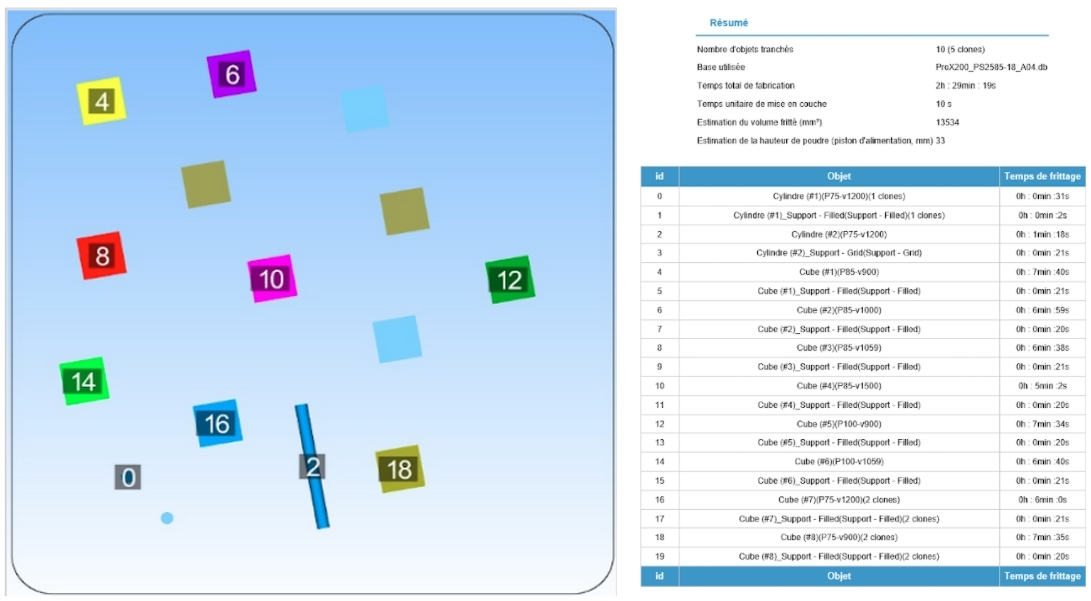
\includegraphics[scale=0.58]{Images/171024-cad}}
\decoRule
\caption[Specimens positions, order of fabrication and sintering times for batch X200-171024]{Specimens positions, order of fabrication and sintering times for batch X200-171024}
\label{fig:171024-cad}
\end{figure}

\begin{figure}[ht]
\centering
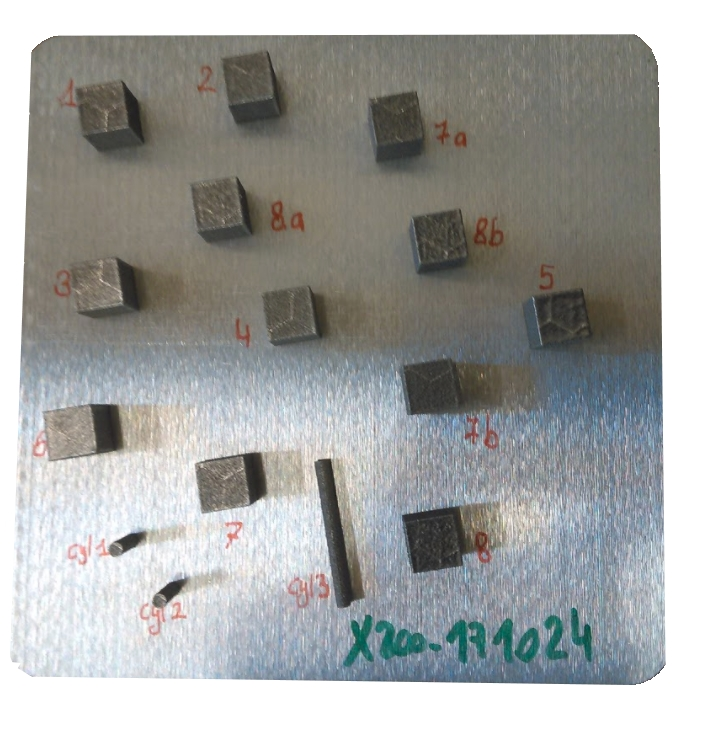
\includegraphics[scale=0.45]{Images/171024-real}
\decoRule
\caption[Photography of the manufacturing plate after completion of the fabrication of batch X200-171024]{Photography of the manufacturing plate after completion of the fabrication of batch X200-171024}
\label{fig:171024-real}
\end{figure}


\subsection{Batch X200-180109}

\begin{figure}[ht]
\centering
\noindent\makebox[\textwidth]{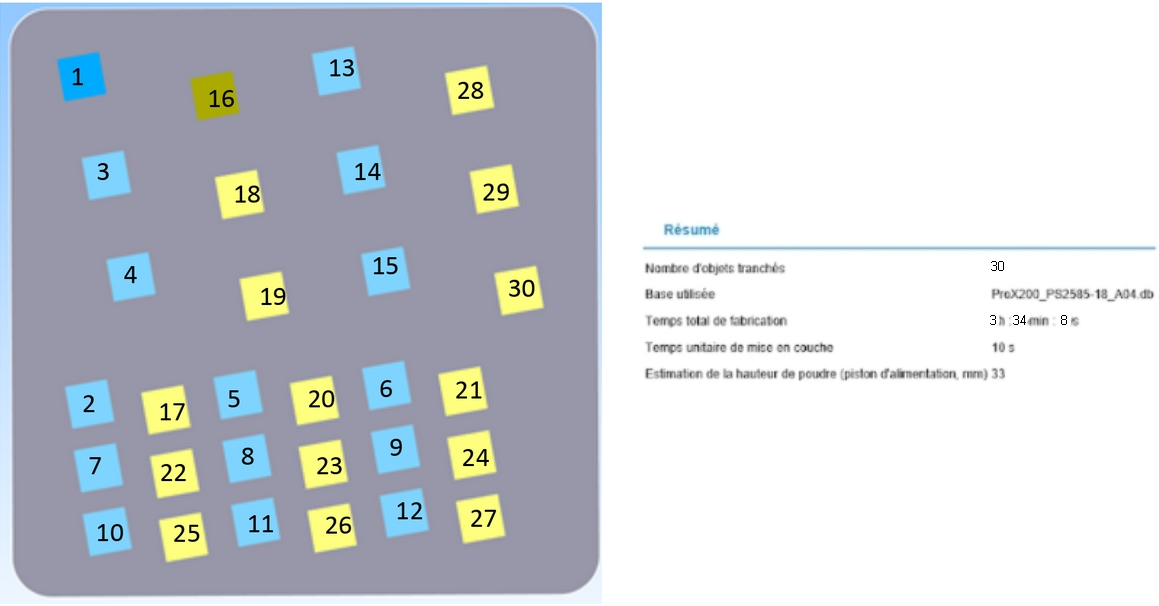
\includegraphics[scale=0.58]{Images/180109-cad}}
\decoRule
\caption[Specimens positions, order of fabrication and sintering times for batch X200-180109]{Specimens positions, order of fabrication and sintering times for batch X200-180109}
\label{fig:171024-cad}
\end{figure}

\begin{figure}[ht]
\centering
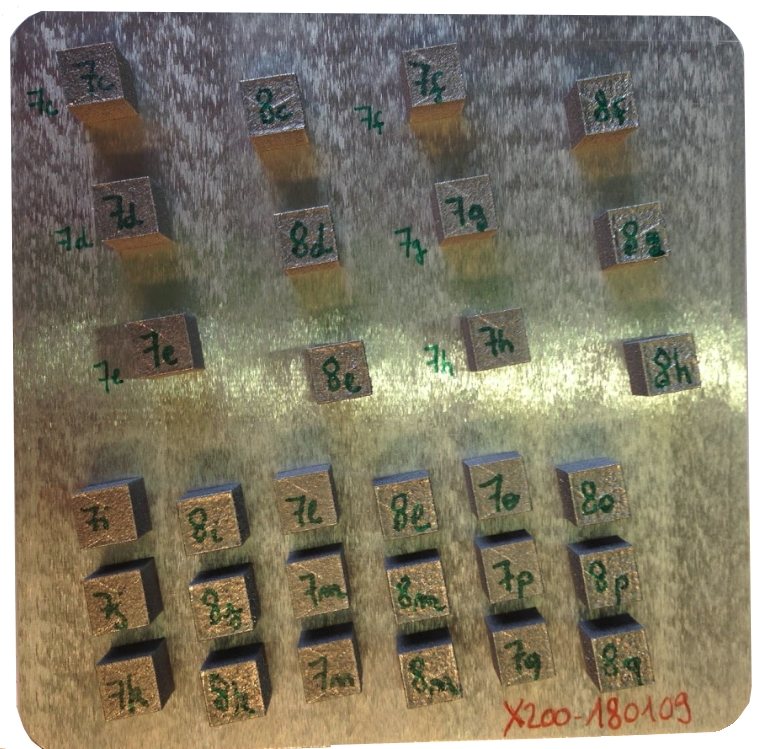
\includegraphics[scale=0.45]{Images/180109-real}
\decoRule
\caption[Photography of the manufacturing plate after completion of the fabrication of batch X200-180109]{Photography of the manufacturing plate after completion of the fabrication of batch X200-180109}
\label{fig:180109-real}
\end{figure}

\subsection{...Other batches}
% Appendix Abis

\chapter{Tensile properties details} % Main appendix title

\label{AppendixAbis} % For referencing this appendix elsewhere, use \ref{AppendixA}
The measured tensile properties for every tested specimens are gathered in this section. Young's modulus values that are in parenthesis were not used in the average computations of sections \ref{RCABS} and \ref{RCHTS}, as the corresponding samples slipped between the grips during the tests. A non-linear behaviour was indeed observed.
\section{As-built samples}

 \begin{center}
\begin{table}[ht]
\noindent\makebox[\textwidth]{\begin{tabular}{|c|c|c |c |c| c|}
    \hline
    Specimen & Contour & E [GPa] & $\sigma_y$ [MPa] & $\sigma_u$ [MPa] & $\epsilon_f$[\%] \\

\hline
\hline   
    X200-180417-1 & Yes  & (74.6) & 271.8 & 366.4 & 2.2  \\
    X200-180417-2 & Yes  & 68.2 & 291.4 & 388.3 & 2.4\\
    X200-180417-3 & Yes  & 64.7 & 276 & - & - \\    
    
    X200-180417-16 & Yes  & 64.7  & 259.3 & 368.0 &2.3 \\ 
    
    X200-180417-17 & Yes  & 66.1   & 255.4  &  406.4&3.0  \\ 
    
    X200-180417-A & No  & 62.0 &255.3  & 379.2 & 2.8 \\
    
    \hline
\end{tabular}}

\caption[Tensile mechanical properties of the as-built specimens from batch X200-180417]{Tensile mechanical properties of the as-built specimens from batch X200-180417}
\label{tab:tracAB}
\end{table}
 \end{center}

\subsection{Heat treated samples}

 \begin{center}
\begin{table}[ht]
\noindent\makebox[\textwidth]{\begin{tabular}{|c|c|c |c |c| c|c|}
    \hline
    Specimen & Contour &  HT & E [GPa] & $\sigma_y$ [MPa] & $\sigma_u$ [MPa] & $\epsilon_f$[\%] \\

\hline
\hline   
    X200-180417-13 & Yes & 150$^\circ$C (2h) & 70.9  & 290.2 & 436.2 & 5.1  \\    
    X200-180417-14 & Yes & 150$^\circ$C (2h) & 67.9 & 286.8  &442.7  & 5.2  \\    
    %X200-180417-15 & Yes & 150$^\circ$C (2h) &  &  &  &  \\    
    X200-180417-B & Yes & 150$^\circ$C (2h) & 66.5 & 287.6  & 446.2 &6.3  \\    
    X200-180417-10 & Yes & 200$^\circ$C (2h) &72.5  &245.9  & 393.4  &4.9  \\    
    X200-180417-11 & Yes & 200$^\circ$C (2h) &71.7  &244.8  &370.6  &4.3  \\    
    %X200-180417-12 & Yes & 200$^\circ$C (2h) &  &  &  &  \\    
    X200-180417-7 & Yes& 250$^\circ$C (2h) & 71.3 & 231.1 & 334.5 & 16.6 \\ % 9.1 \\
    X200-180417-8 & Yes& 250$^\circ$C (2h) & 69.6 & 239.2 & 347.4 &16.4\\% 8.6 \\
    X200-180417-9 & Yes& 250$^\circ$C (2h) & 71.0 & 227.7 &$\simeq 328.7$ & - \\
    X200-180417-4 & Yes& 300$^\circ$C (2h) & (81.6) & 168.9 & 249.6 &29.6\\% 14.1 \\ 
    X200-180417-5 & Yes& 300$^\circ$C (2h) & 68.3 &172.4 & 256.24 &29.8 \\%13.1 \\
    X200-180417-6 & Yes& 300$^\circ$C (2h) & 69.5 &168.5 & $\simeq 242.5$ & - \\

\hline
\end{tabular}}

\caption[Tensile mechanical properties of the heat treated specimens from batch X200-180417]{Tensile mechanical properties of the heat treated specimens from batch X200-180417}
\label{tab:tracTT}
\end{table}
 \end{center}


% Appendix B

\chapter{Extract of Vickers hardness conversion table (HV10)} % Main appendix title

\label{AppendixB} % For referencing this appendix elsewhere, use \ref{AppendixA}

\begin{center}
\begin{table}[ht]
\noindent\makebox[\textwidth]{\begin{tabular}{|c|c |c |c| c|c|c|c|c|c|c|}
    \hline
    Diagonal length [mm] & 0 &1&2&3&4&5&6&7&8&9\\
\hline 
\hline   
    0.34 & 160 &160&159&158&157&156&155&154&153&152\\
    0.35&151.4&150.5&149.7&148.8&148.0&147.1&146.3&145.5&144.7&143.9\\ 
    0.36&143.1&142.3&141.5&140.7&140.0&139.2&138.4&137.7&136.9&136.2\\
    0.37&135.5&134.7&134.0&133.3&132.6&131.9&131.2&130.5&129.8&129.1\\
    0.38&128.4&127.7&127.1&126.4&125.8&125.1&124.5&123.8&123.2&122.6\\
    0.39&121.9&121.3&120.7&120.1&119.5&118.9&118.3&117.7&117.1&116.5\\
    0.40&115.9&115.3&114.8&114.2&113.6&113.1&112.5&111.9&111.4&110.9\\
    0.41&110.3&109.8&109.3&108.7&108.2&107.7&107.2&106.6&106.1&105.6\\
    0.42&105.1&104.6&104.1&103.6&103.1&102.7&102.2&101.7&101.2&100.8\\
    0.43&100.3&99.8&99.4&98.9&98.5&98.0&97.6&97.1&96.7&96.2\\
    0.44&95.8&95.3&94.9&94.5&94.1&93.6&93.2&92.8&92.4&92.0\\
    0.45&91.6&91.2&90.8&90.4&90.0&89.6&89.2&88.8&88.4&88.0\\
    0.46&87.6&87.3&86.9&86.5&86.1&85.8&85.4&85.0&84.7&85.3\\
    0.47&84.0&83.6&83.2&82.9&82.5&82.2&81.8&81.5&81.2&80.8\\
    0.48&80.5&80.2&79.8&79.5&79.2&78.8&78.5&78.2&77.9&77.6\\
    0.49&77.2&76.9&76.6&76.3&76.0&75.7&75.4&75.1&74.8&74.5\\
    0.50&74.2&73.9&73.6&73.3&73.0&72.7&72.4&72.1&71.9&71.6\\
    0.51&71.3&71.0&70.7&70.5&70.2&69.9&69.6&69.4&69.1&68.8\\
    0.52&68.6&68.3&68.1&67.8&68.5&67.3&67.0&66.8&66.5&66.3\\
    0.53&66.0&65.8&65.5&65.3&65.0&64.8&64.5&64.3&64.1&63.8\\
    0.54&63.6&63.4&63.1&62.9&62.7&62.4&62.2&62.0&61.7&61.5\\    \hline
\end{tabular}}

\caption[Extract of Vickers hardness conversion table (HV10)]{Extract of Vickers hardness conversion table (HV10)}
\label{tab:compo}
\end{table}
 \end{center}

% Appendix B

\chapter{Procedure for the confidence intervals computation} % Main appendix title

\label{AppendixC} % For referencing this appendix elsewhere, use \ref{AppendixA}

\section{Hydrostatic weighting}

The hydrostatic weighting method requires to weight the analysed samples two times; once in air and once in water. The measurements data of the two weightings are subjected to a certain spreading - especially large in the case of underwater measurements. Both of the tests imprecisions must thus be taken into account when computing the confidence intervals (CI) for $\rho_{a,rel}$. The following procedure was followed:

\begin{itemize}
\item Computation of the standard deviation $SD_x$ for the two data samples of observed mass values \{$x_1$,$x_2$,...$x_N$\} with the formula below:

$$SD_x=\sqrt{\frac{\Sigma^N_{i=1}(x_i-\bar{x})^2}{N-1}} $$

where is N the sample size and $\bar{x}$ is the mean of the observed values.

\item Determination of the CI range at a 95 [\%] confidence level for each data sample with the following formula:

$$CI= \bar{x} \pm 1.96 \frac{SD_x}{\sqrt{N}}$$

\item Use of the mean values incremented by the extreme values of the CI for both $W_a$ and $W_w$ in the formula:


$$\rho_a=\frac{W_a}{W_a-W_w} \cdot \rho_w $$

so as to maximise the absolute value of the difference with $\bar{x}$. This difference is then equal to the CI half length for a 95 [\%] confidence level.
\end{itemize}

\section{Vickers hardness}

Hardness measurements of a given sample are also prone to having a certain variability. CI must thus be computed to assess the method precision. The CI is first calculated for the data sample composed of the mean diagonals length of the indents. For this purpose, one follows the same two first steps as for the hydrostatic weighting. The CI range is then multiplied by 800 to find the hardness's one. This is done in accordance with the observation that the maximal hardness variation for a change of 0.001 [mm] is 0.8 [HV] in table \ref{tab:HV} for $H_v<147.1 $[HV].% This is the origin of the factor 800. 
% Appendix B

\chapter{Reproducibility study additional plots} % Main appendix title

\label{AppendixD} % For referencing this appendix elsewhere, use \ref{AppendixA}

\begin{figure}[ht]
\centering
\centerline{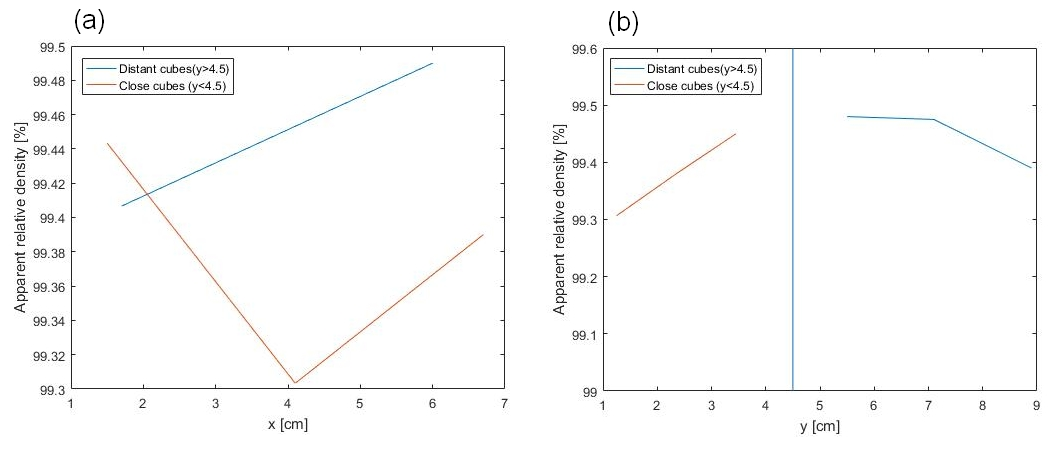
\includegraphics[scale=0.55]{Images/180109-7Dxy}}
\decoRule
\caption[Average apparent relative density of batch X200-180109 type "7" samples as a function of the (a) x coordinate (b) y coordinate]{Apparent relative density of batch X200-180109 type "7" samples as a function of the (a) x coordinate (b) y coordinate}
\label{180109-7Dxy}
\end{figure} 

\begin{figure}[ht]
\centering
\centerline{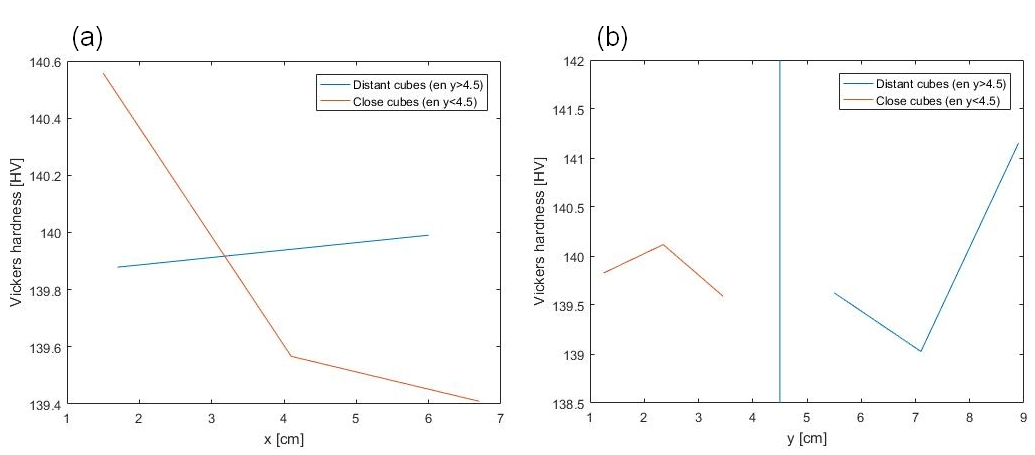
\includegraphics[scale=0.55]{Images/180109-7Hxy}}
\decoRule
\caption[Average Vickers hardness of batch X200-180109 type "7" samples as a function of the (a) x coordinate (b) y coordinate]{Vickers hardness of batch X200-180109 type "7" samples as a function of the (a) x coordinate (b) y coordinate}
\label{180109-7Hxy}
\end{figure} 

\begin{figure}[ht]
\centering
\centerline{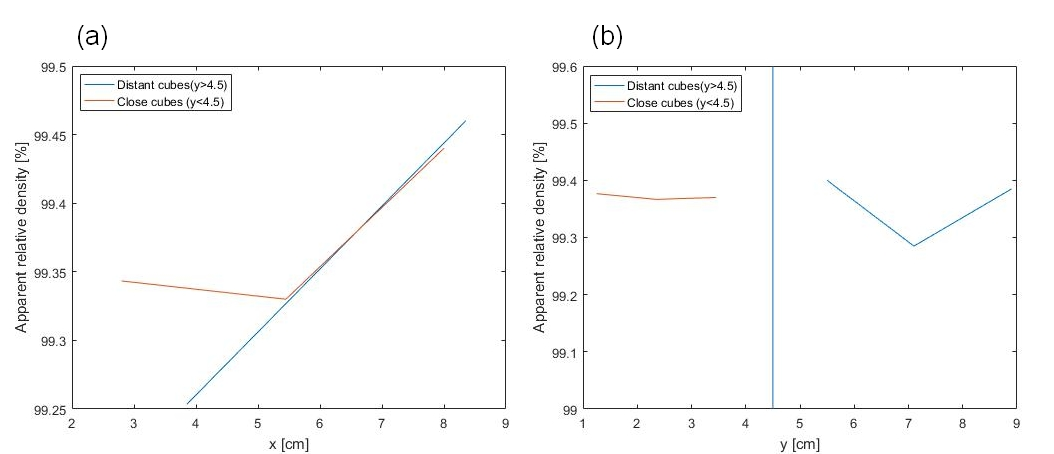
\includegraphics[scale=0.55]{Images/180109-8Dxy}}
\decoRule
\caption[Average apparent relative density of batch X200-180109 type "8" samples as a function of the (a) x coordinate (b) y coordinate]{Apparent relative density of batch X200-180109 type "8" samples as a function of the (a) x coordinate (b) y coordinate}
\label{180109-8Dxy}
\end{figure} 

\begin{figure}[ht]
\centering
\centerline{\includegraphics[scale=0.55]{Images/180109-8Hxy}}
\decoRule
\caption[Average Vickers hardness of batch X200-180109 type "8" samples as a function of the (a) x coordinate (b) y coordinate]{Vickers hardness of batch X200-180109 type "8" samples as a function of the (a) x coordinate (b) y coordinate}
\label{180109-8Hxy}
\end{figure} 
%----------------------------------------------------------------------------------------
%	BIBLIOGRAPHY
%----------------------------------------------------------------------------------------

\printbibliography[heading=bibintoc]

%----------------------------------------------------------------------------------------

\end{document}
